\documentclass[unknownkeysallowed]{beamer}\usepackage[]{graphicx}\usepackage[]{color}
% maxwidth is the original width if it is less than linewidth
% otherwise use linewidth (to make sure the graphics do not exceed the margin)
\makeatletter
\def\maxwidth{ %
  \ifdim\Gin@nat@width>\linewidth
    \linewidth
  \else
    \Gin@nat@width
  \fi
}
\makeatother

\definecolor{fgcolor}{rgb}{0.345, 0.345, 0.345}
\newcommand{\hlnum}[1]{\textcolor[rgb]{0.686,0.059,0.569}{#1}}%
\newcommand{\hlstr}[1]{\textcolor[rgb]{0.192,0.494,0.8}{#1}}%
\newcommand{\hlcom}[1]{\textcolor[rgb]{0.678,0.584,0.686}{\textit{#1}}}%
\newcommand{\hlopt}[1]{\textcolor[rgb]{0,0,0}{#1}}%
\newcommand{\hlstd}[1]{\textcolor[rgb]{0.345,0.345,0.345}{#1}}%
\newcommand{\hlkwa}[1]{\textcolor[rgb]{0.161,0.373,0.58}{\textbf{#1}}}%
\newcommand{\hlkwb}[1]{\textcolor[rgb]{0.69,0.353,0.396}{#1}}%
\newcommand{\hlkwc}[1]{\textcolor[rgb]{0.333,0.667,0.333}{#1}}%
\newcommand{\hlkwd}[1]{\textcolor[rgb]{0.737,0.353,0.396}{\textbf{#1}}}%
\let\hlipl\hlkwb

\usepackage{framed}
\makeatletter
\newenvironment{kframe}{%
 \def\at@end@of@kframe{}%
 \ifinner\ifhmode%
  \def\at@end@of@kframe{\end{minipage}}%
  \begin{minipage}{\columnwidth}%
 \fi\fi%
 \def\FrameCommand##1{\hskip\@totalleftmargin \hskip-\fboxsep
 \colorbox{shadecolor}{##1}\hskip-\fboxsep
     % There is no \\@totalrightmargin, so:
     \hskip-\linewidth \hskip-\@totalleftmargin \hskip\columnwidth}%
 \MakeFramed {\advance\hsize-\width
   \@totalleftmargin\z@ \linewidth\hsize
   \@setminipage}}%
 {\par\unskip\endMakeFramed%
 \at@end@of@kframe}
\makeatother

\definecolor{shadecolor}{rgb}{.97, .97, .97}
\definecolor{messagecolor}{rgb}{0, 0, 0}
\definecolor{warningcolor}{rgb}{1, 0, 1}
\definecolor{errorcolor}{rgb}{1, 0, 0}
\newenvironment{knitrout}{}{} % an empty environment to be redefined in TeX

\usepackage{alltt}

\usetheme{default}
\useoutertheme{infolines}
\setbeamertemplate{navigation symbols}{} 
\setbeamertemplate{footline}[frame number]
\setbeamertemplate{headline}{}

\usepackage{amsmath}
\usepackage{statrep}
\usepackage{parskip,xspace}
\newcommand*{\Statrep}{\mbox{\textsf{StatRep}}\xspace}
\newcommand*{\Code}[1]{\texttt{\textbf{#1}}}
\newcommand*{\cs}[1]{\texttt{\textbf{\textbackslash#1}}}
\setcounter{secnumdepth}{0}
\def\SRrootdir{.}
\def\SRmacropath{./statrep_macros.sas}
\newcommand{\mytilde}{\raise.17ex\hbox{$\scriptstyle\mathtt{\sim}$}}
\usepackage[utf8]{inputenc}
% \DeclareUnicodeCharacter{00D7}{$\times$}
% \DeclareUnicodeCharacter{221A}{\checkmark}
\usepackage{graphicx}
\usepackage{hyperref}
\usepackage{multicol}
\usepackage{pbox}
\usepackage{verbatim}

\title{STAC32}
\subtitle{Applications of Statistical Methods}
\author{Ken Butler}
\IfFileExists{upquote.sty}{\usepackage{upquote}}{}
\begin{document}

%\maketitle





% installing our software


\section{Connecting to SAS}

\frame{\sectionpage}


\begin{frame}{Recall history}
  
  \begin{tabular}{p{0.45\textwidth}p{0.49\textwidth}}
    \textbf{SAS} & \textbf{R}\\
    From late 1960s, North Carolina State.&
From 1993, New Zealand.\\                                            
    Then: punched cards, ``submit'' job, get output later.
    Still SAS's way of operating: run list of commands, get lot
      of output.& R style: enter commands one at a time, see output/graphics
      right away.\\
                 
    Commercialized, corporate ethos.             & Open-source, free. Core group, anyone can contribute.\\
    Strength: Submitting same commands again gets \emph{exactly}
      same results. (Government, industry).& 
    Grew out of commercial software S, which appeared when
      graphics terminals new (emphasis on graphics).\\
                                             & Concept of ``function'' lets you add onto R or do
      non-standard things.\\
    Long history: well-tested.&Big user community makes sure everything works.
    
  \end{tabular}
  
  \end{frame}

%% \begin{frame}{Installing R}
%% 
%%   \begin{itemize}
%%   \item Free, open-source. Download and run on own computer.
%%   \item Two things: R itself (install first) and R Studio (front end).
%%     \item Go to \url{https://www.r-project.org/}:
%%       
%%       
\includegraphics[width=4in]{r30}
%%   \end{itemize}
%%   
%% \end{frame}
%% 
%% \begin{frame}[fragile]{Click on Download}
%%   
%%   \begin{itemize}
%%   \item R is stored on numerous ``mirrors'', sites around the
%%     world. Choose one close to you (faster), eg.\ U of T:
%%     
%%     
\includegraphics[width=4in]{r39}
%%   \end{itemize}
%%   
%% \end{frame}
%% 
%% 
%% \begin{frame}[fragile]{Click U of T}
%%   
%%   \begin{itemize}
%%   \item Click U of T (or other mirror), get:
%%     
%%     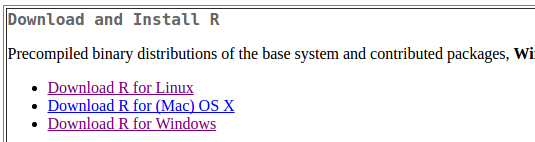
\includegraphics[width=4in]{r32}
%%     
%%     \item Click on your operating system, eg.\ Windows.
%%   \end{itemize}
%%   
%% \end{frame}
%% 
%% \begin{frame}[fragile]{Click on Base}
%% 
%%       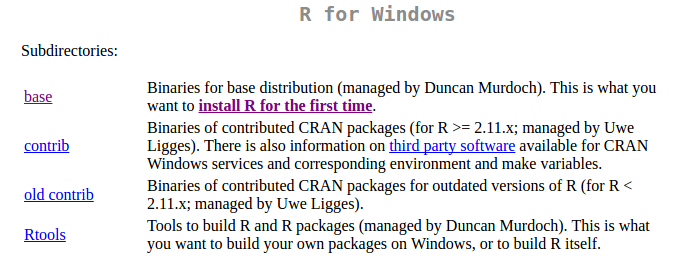
\includegraphics[width=4in]{r33}
%% 
%%   \begin{itemize}
%%   \item Click on ``base'' here.
%%   \end{itemize}
%%   
%% \end{frame}
%% 
%% 
%% \begin{frame}[fragile]{The actual download}
%%   
%%   \begin{itemize}
%%   \item Click the top link below:
%%     
%%     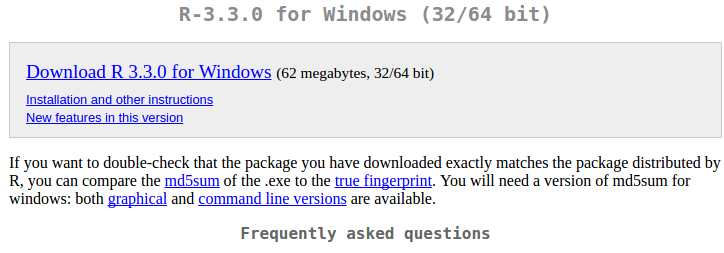
\includegraphics[width=4in]{r34}
%%     
%%   \item Then install usual way.
%%   \end{itemize}
%%   
%% \end{frame}
%% 
%% 
%% \begin{frame}[fragile]{Now, R Studio}
%%   
%%   \begin{itemize}
%%   \item Go to \url{https://www.rstudio.com/}.
%%   \item Scroll down to this, and click Learn More (the left one):
%%     
%%     
\includegraphics[width=3in]{r35}
%%   \end{itemize}
%%   
%% \end{frame}
%% 
%% \begin{frame}[fragile]{Scroll down}
%%   
%%   \begin{itemize}
%%   \item Scroll down to this:
%%     
%%     
\includegraphics[width=4in]{r37}
%%     
%%   \item Click ``Download RStudio Desktop''.
%%   \end{itemize}
%%   
%% \end{frame}
%% 
%% \begin{frame}[fragile]{Find the one for you}
%%   
%%   \begin{itemize}
%%   \item Scroll down, and click the installer for your machine
%%     (Windows, Mac, 4 flavours of Linux). Install as usual.
%%     
%%     \includegraphics[width=4in]{r40}
%%   \end{itemize}
%%   
%% \end{frame}
%% 
%% 
%% \begin{frame}[fragile]{Running R}
%%   
%%   \begin{itemize}
%%   \item All of above only done \emph{once}.
%%   \item To run R, run \textbf{R Studio}, which itself runs R.
%%   \end{itemize}
%%   
%% \end{frame}
%% 
%% \begin{frame}[fragile]{How R Studio looks when you run it}
%%   
%% 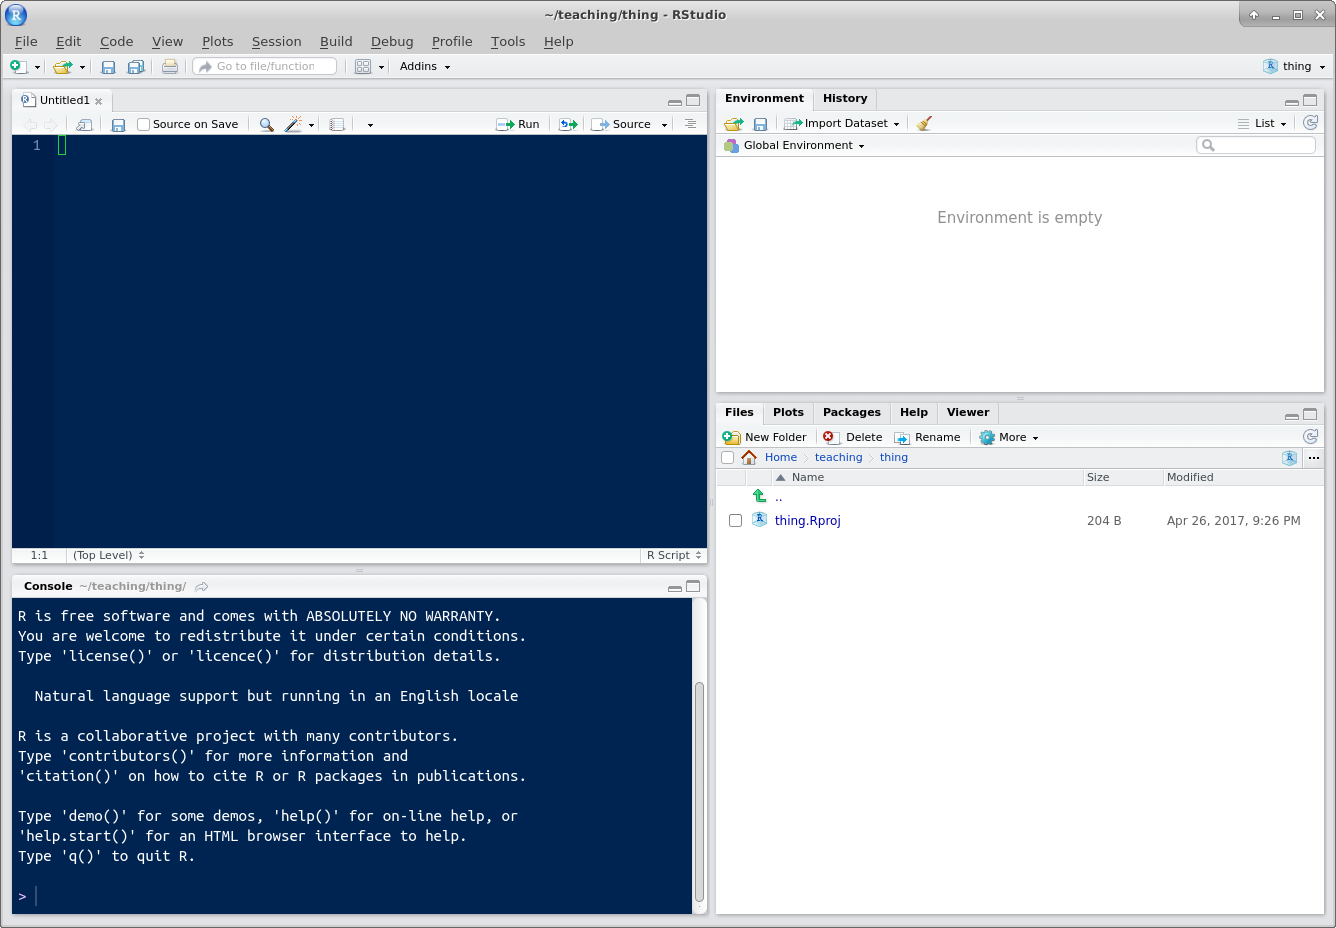
\includegraphics[width=0.8\textwidth]{rstudio-startup}
%%   
%% First time you run R Studio, click on Console window, and, next to the
%% \texttt{>}, type \texttt{install.packages("tidyverse")}. Let it do
%% what it needs to.
%% \end{frame}


\begin{frame}[fragile]{Connecting to SAS}

  \begin{itemize}
  \item SAS on your own computer big, expensive.
  \item U of T has ``site licence'' allows us to buy SAS for own
    computer (re-licensed every year, etc.)
  \item SAS offers ``SAS Studio'' that is free for the academic
    world. This runs through a web browser (accessible everywhere)
    with everything hosted on SAS's servers, or on a ``virtual
    machine'' on own computer.
  \item The hard part is getting registered for it.
  \end{itemize}
  
\end{frame}

\begin{frame}[fragile]{Getting registered for online version}

  \begin{itemize}
  \item Go to \url{https://odamid.oda.sas.com}. Get to this:

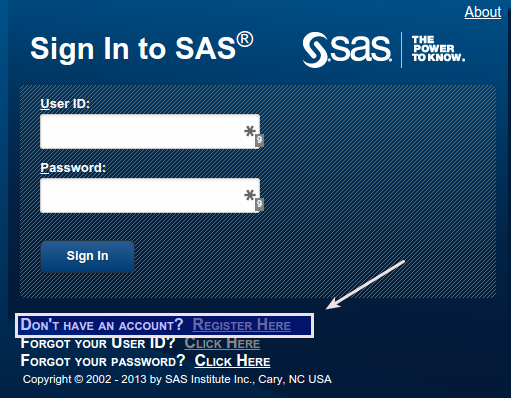
\includegraphics[height=0.6\textheight]{sas1}

\item Bookmark this page.
\item Go down to ``Don't have an account?'' and click ``Register Here''.
  \end{itemize}
  
\end{frame}

\begin{frame}[fragile]{Enter your name and e-mail}

\ldots and select country (Canada):

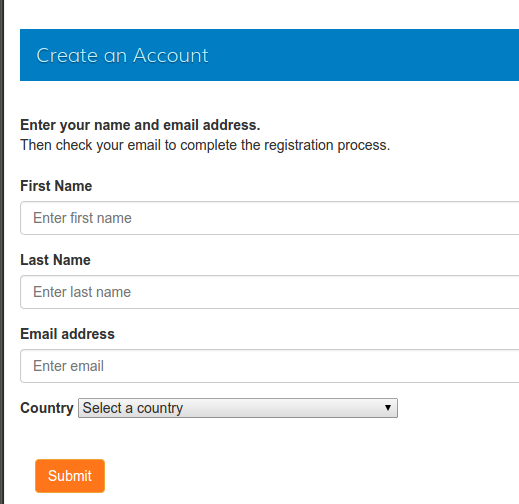
\includegraphics[width=3in]{sas2}
  
\end{frame}

\begin{frame}[fragile]{Go check your e-mail}

and look for something like this:

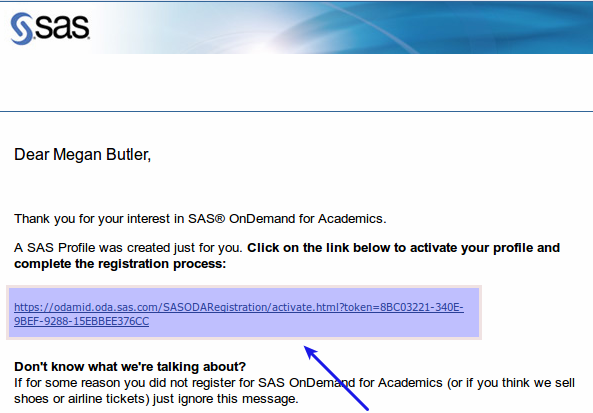
\includegraphics[width=3in]{sas3}

Click on the link.
  
\end{frame}

\begin{frame}[fragile]{Choose a password}

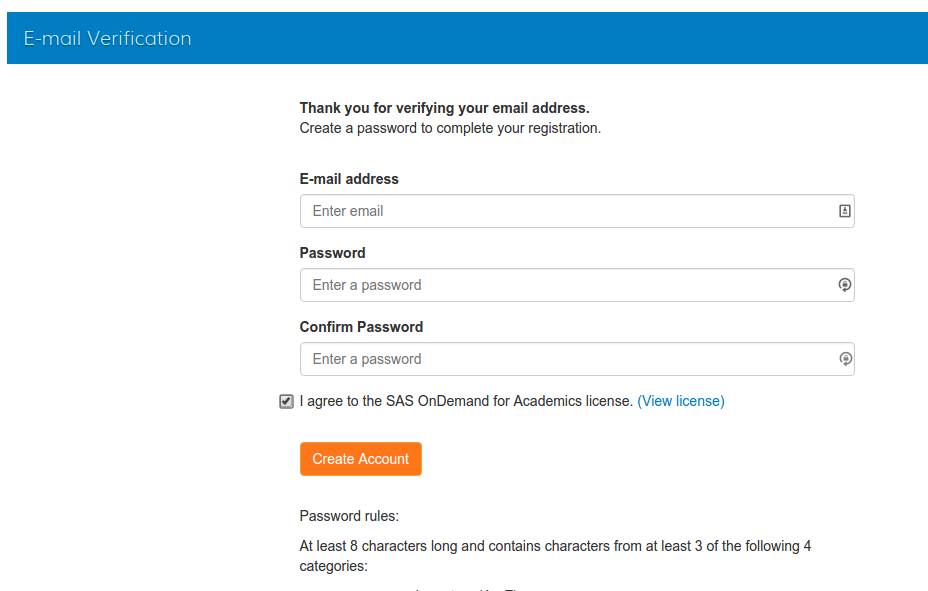
\includegraphics[height=0.7\textheight]{sas5}

  \begin{itemize}
  \item Click orange Create Account. You then get a user ID. Make a note of it.
  \item This completes the registration. You only do this once.
  \end{itemize}
  
\end{frame}

\begin{frame}[fragile]{Log into SAS}

Go back to the page you bookmarked earlier:

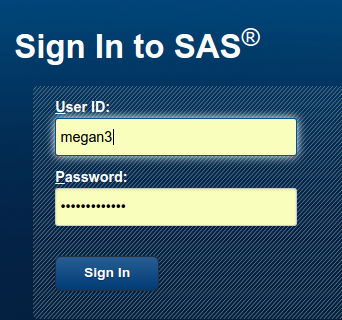
\includegraphics[height=0.7\textheight]{sas1b}

Type your user ID and password into the boxes, and click Sign In.
  
\end{frame}


\begin{frame}[fragile]{The dashboard}

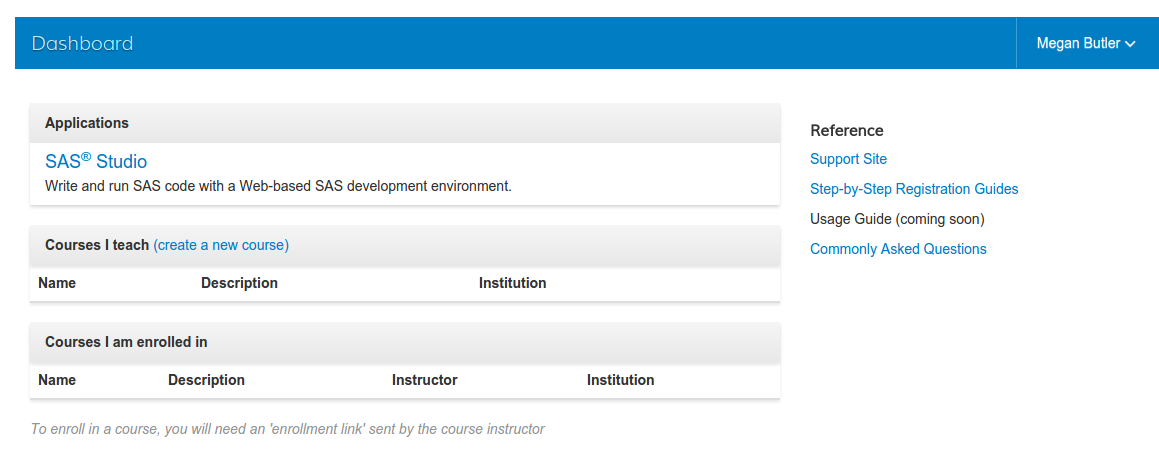
\includegraphics[width=\textwidth]{sas6}

On the Dashboard, click SAS Studio. (Ignore the stuff about the
courses.) 
  
\end{frame}

\begin{frame}[fragile]{SAS, as you see it}

Something like this:

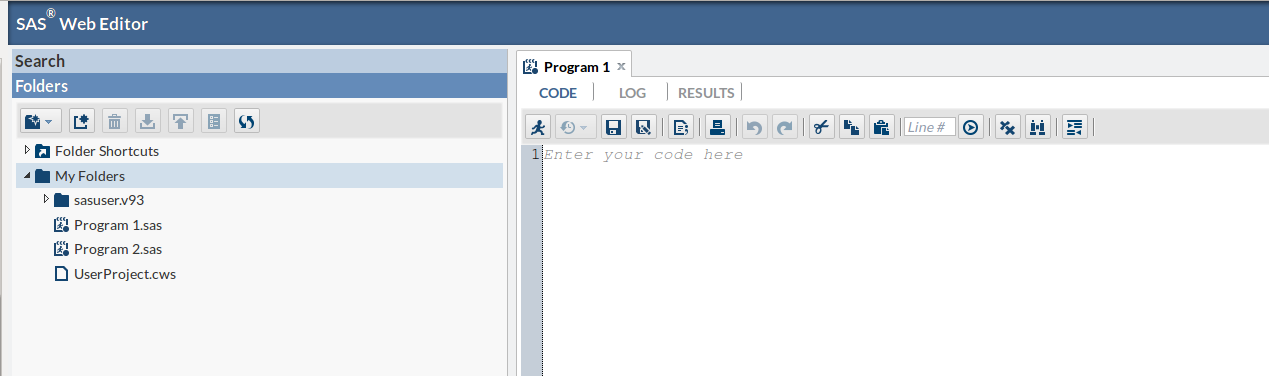
\includegraphics[scale=0.3]{sas-webed-opening}
  
\end{frame}


%\begin{frame}[fragile]{Trying out SAS}
%
%Go to the right side of the window, under Program 1, click on Code,
%and type the following into the window with the numbered lines:
%
%\includegraphics[scale=0.4]{prog1}
%
%When you have this to your satisfaction, click the ``running
%humanoid'' under Code. (This is called ``submitting'' in SAS jargon.)
% 
%\end{frame}
%
%\begin{frame}[fragile]{Output}
%
%If everything was correct, the Results tab under Program 1 will be
%selected, and you'll see your results, thus:
%
%\includegraphics[scale=0.35]{results1}
%
%These are: a listing of your data (from \texttt{proc print}) and a
%summary of the data, including mean and SD (from \texttt{proc means}).
%  
%\end{frame}
%
%\begin{frame}[fragile]{Errors}
%  
%  \begin{itemize}
%  \item Let me make a deliberate mistake: I left off the semicolon on the end
%of \texttt{proc print}.
%\item  When I submitted this, the Log tab popped up
%with a whole bunch of stuff including this:
%
%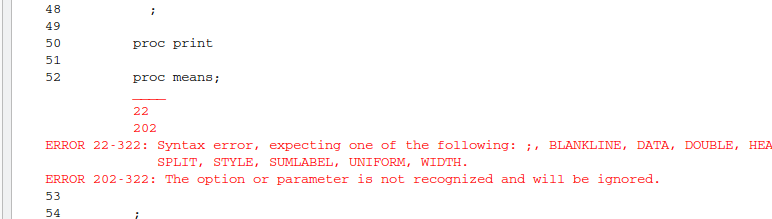
\includegraphics[scale=0.35]{sas-error}
%
%\item When SAS hit \texttt{proc means}, expecting a semicolon (to
%finish off the \texttt{proc print;}), but didn't see one. So error
%was \emph{just before} where the mark was. 
%
%\item Tactic: fix the \emph{first} error and submit again. (That
%first error might have caused a bunch of others.)  
%
%  \end{itemize}
%
%
%
%
%\end{frame}


\begin{frame}[fragile]{Installing SAS on your own machine}

  \begin{itemize}
  \item Pro: not dependent on SAS's servers.
  \item Con: fiendishly complicated!
  \item On your own computer, SAS runs in ``virtual machine'' (so
    doesn't matter what OS you have, as long as the virtual machine
    runs on it).
  \end{itemize}
  
\end{frame}

%%%%%%%%%%%%% 2016 version

\begin{frame}[fragile]{Getting SAS for your own machine}
  
  \begin{itemize}
  \item Go to \url{sas.com} and navigate to Products and Solutions,
    then SAS University Edition, or
    go to \url{http://www.sas.com/en_ca/software/university-edition.html}.
  \item See this:
    
    
\includegraphics[width=4in]{sas16}
  \end{itemize}
  
\end{frame}

\begin{frame}[fragile]{And then}
  
  \begin{itemize}
  \item Click Get Free Software. See this:
    
    
\includegraphics[width=3in]{sas28}
    
  \item Click Download Now on the \emph{left}.
  \end{itemize}
  
\end{frame}

\begin{frame}[fragile]{Select operating system}
  
  \begin{itemize}
  \item by clicking appropriate tab, eg:
    
    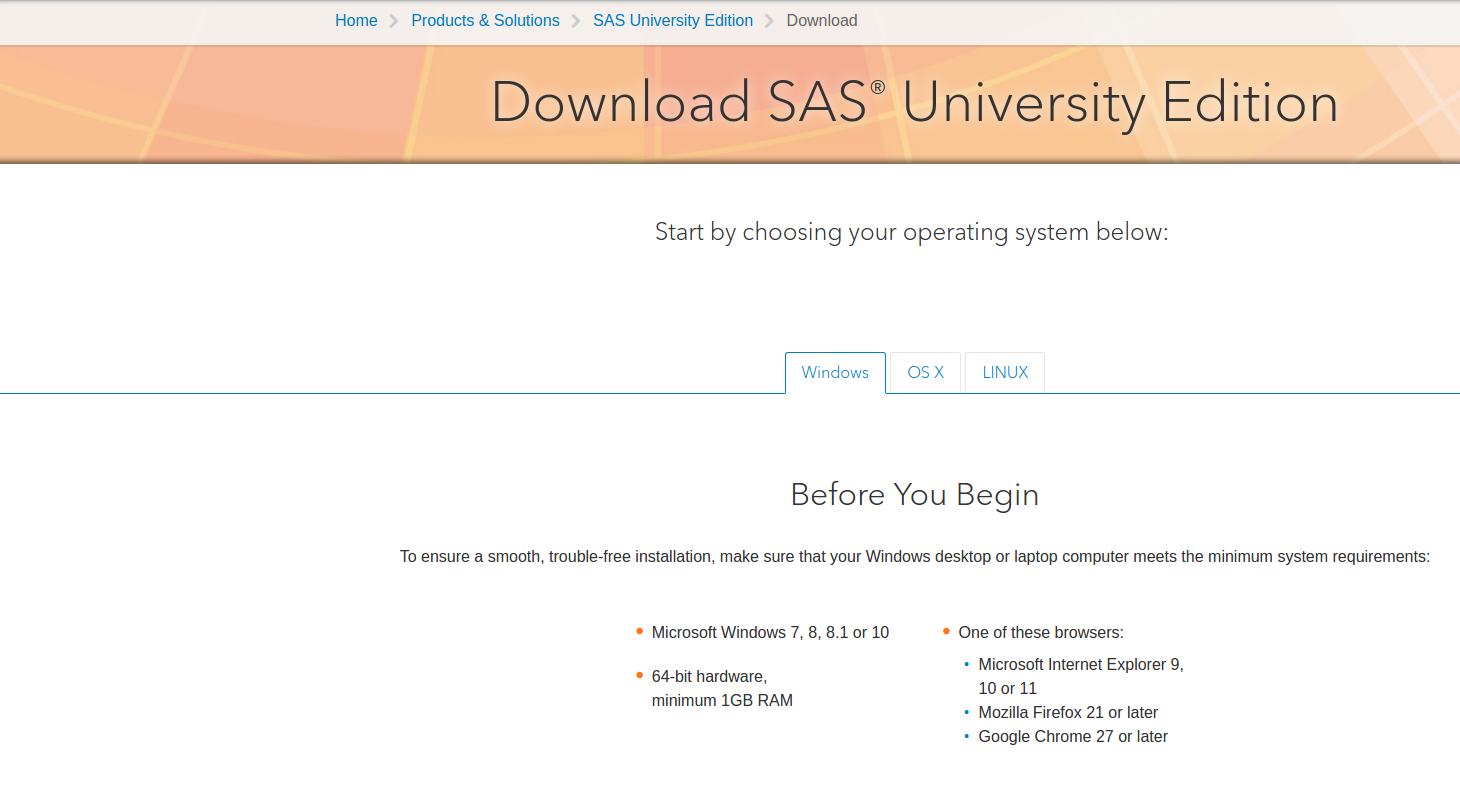
\includegraphics[width=4in]{sas17}
  \end{itemize}
  
\end{frame}

\begin{frame}[fragile]{Starting setup}
  
  \begin{itemize}
  \item Click tab for your operating system, and check that your
    system is good.
  \item Scroll down (4 steps):
    
    
\includegraphics[width=3.5in]{sas18}
    
  \end{itemize}
  
\end{frame}

\begin{frame}[fragile]{Download VirtualBox}
  
  \begin{itemize}
  \item SAS runs on ``virtual machine'' (has own operating system
    regardless of what yours is). Download and install virtual machine:
    
    
\includegraphics[width=4in]{sas19}
  \end{itemize}
  
\end{frame}


\begin{frame}[fragile]{Scroll down some more}
  
  \begin{itemize}
  \item You will be downloading a 1.7GB ``app'' (this may take a while). You may
    have to create a username/password first (next page):
    
    
\includegraphics[width=2.5in]{sas20}
  \end{itemize}
  
  
\end{frame}

\begin{frame}[fragile]{Creating a ``profile''}
  
  \begin{itemize}
  \item New User on the right (unless you already have a SAS profile):

      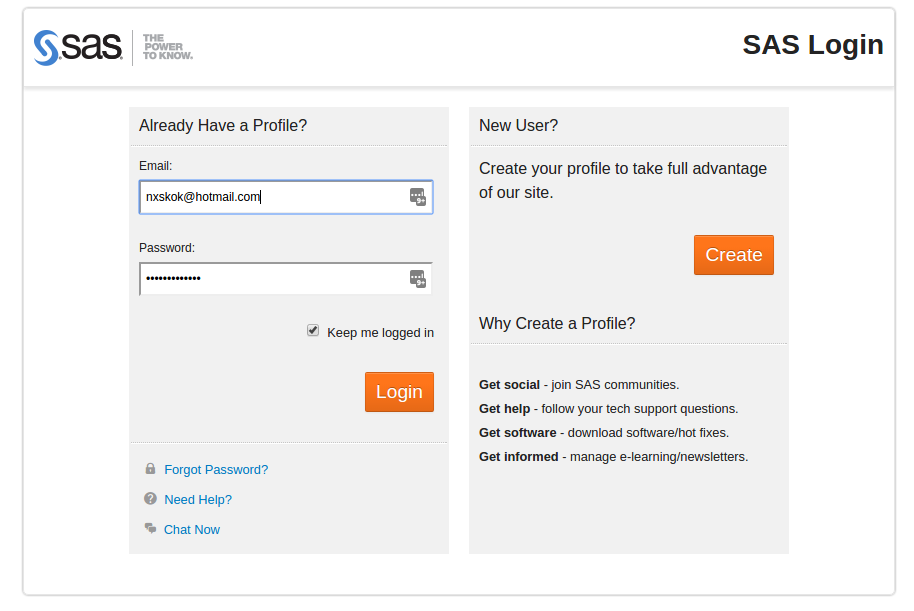
\includegraphics[width=4in]{sas22}

  \end{itemize}
  
  
\end{frame}

\begin{frame}[fragile]{Finally, step 4}
  
  \begin{itemize}
  \item Follow the steps in the Quick Start Guide. Step 1 you probably
    already did:
    
    
\includegraphics[width=4in]{sas23}
  \end{itemize}
  
\end{frame}

\begin{frame}[fragile]{Quick Start step 2}
  
  \begin{itemize}
  \item Follow the instructions. This attaches the ``app'' to your
    virtual machine so that it will run:
    
    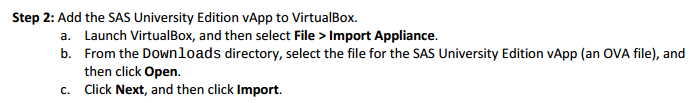
\includegraphics[width=4in]{sas24}
  \end{itemize}
  
\end{frame}

\begin{frame}[fragile]{Step 3: setting up file access}
  
  \begin{itemize}
  \item This is kind of complicated, but follow the steps through, and
    then you can read in data files:
    
    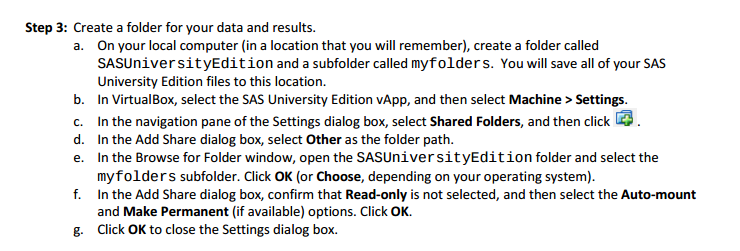
\includegraphics[width=4in]{sas25}
  \end{itemize}
  
\end{frame}

\begin{frame}[fragile]{Start SAS}
  
  \begin{itemize}
  \item All of the above you only do once (installation).
  \item To start SAS, do the below (every time):
    
    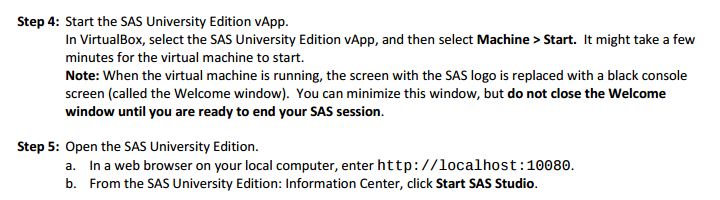
\includegraphics[width=4in]{sas26}
  \end{itemize}
  
\end{frame}


\begin{frame}[fragile]{SAS Studio online and on your machine}

  \begin{itemize}
  \item SAS Studio runs identically whether it's online or on your machine.
  \item With one exception: accessing files (typically data files).
  \item Otherwise, any reference to SAS Studio applies equally well to
    either version.
  \end{itemize}
  
\end{frame}


\begin{frame}[fragile]{Accessing data files in SAS Studio}

    \begin{itemize}
    \item Depends on whether you're running SAS Studio online or on
      your computer.
    \item If you're running online, you have a username that you used
      for logging in, like \texttt{ken} or \texttt{megan3}.
    \item Online: access file as \texttt{/home/} plus your username
      plus filename: eg.\ \texttt{/home/megan3/mydata.txt}.
    \item On your computer: \texttt{/folders/myfolders/} plus
      filename, eg.\ \texttt{/folders/myfolders/mydata.txt}.
    \item Slashes in both cases are \emph{forward} slashes, and you
      need one to start the filename.
    \end{itemize}
    
\end{frame}

%\begin{frame}[fragile]{Using SAS Studio to save a data file}
%
%Works on either version of SAS Studio. 
%
%Create a new ``SAS Program'' (only it won't be) and
%type/copy these, as shown, into the Code window:
%
%\begin{columns}
%  
%  \begin{column}{0.3\textwidth}
%{\small
%\begin{verbatim}
%a 20
%a 21
%a 16
%b 11
%b 14
%b 17
%b 15
%c 13
%c 9
%c 12
%c 13
%\end{verbatim}
%}
%    
%  \end{column}
%
%  \begin{column}{0.65\textwidth}
%\begin{itemize}
%\item Save into file \texttt{three.txt}. Select My Folders as
%  folder to save in. SAS puts \texttt{.sas} on the
%  file name. Find the file in the Folders window, right-click, select
%  Rename, and make the filename what you really wanted.
%\end{itemize}
%    
%  \end{column}
%
%  
%\end{columns}
%
%  
%\end{frame}
%
%
%\begin{frame}[fragile]{Analysis 1(a): reading in and verifying the data}
%
%  \begin{itemize}
%\item This version if you're accessing SAS Studio online.
%\item Create a new SAS program, and enter its code thus (in the Code
%  tab):
%  
%\begin{semiverbatim}
%data groups;
%  infile '/home/ken/three.txt';
%  input group $ y;
%
%proc print;    
%\end{semiverbatim}
%  
%
%\item Replace \texttt{ken} with your online SAS Studio username.
%
%\item Code much cleaner with data in separate file.
%
%  \end{itemize}
%
%
%\end{frame}
%
%
%\begin{frame}[fragile]{Analysis 1(b): reading in and verifying the data}
%
%  \begin{itemize}
%\item This version if you're accessing SAS Studio on your own computer
%  (via virtual machine).
%\item Create a new SAS program, and enter its code thus (in the Code
%  tab):
%  
%  
%
%\begin{Datastep}
%data groups;
%  infile '/folders/myfolders/three.txt';
%  input group $ y;
%\end{Datastep}
%
%\begin{Sascode}[store=threea]
%proc print;  
%\end{Sascode}
%
%
%
%\item We'll see output in a moment. Same both ways.
%  \end{itemize}
%
%
%\end{frame}
%
%\begin{frame}[fragile]{Output}
%  
%\Listing[store=threea]{threeaa}
%
%
%\end{frame}
%
%\begin{frame}[fragile]{Folder menu}
%
%\includegraphics[width=\textwidth]{folder-menu}
%  
%\end{frame}
%
%\begin{frame}[fragile]{Code menu}
%
%\includegraphics[width=\textwidth]{code-menu}
%  
%\end{frame}
%
%
%\begin{frame}[fragile]{Results menu}
%
%\includegraphics[width=\textwidth]{results-menu}
%  
%\end{frame}
%
%
%\begin{frame}{Other notes}
%
%  \begin{itemize}
%
%  \item When saving your code, SAS appends a \texttt{.sas} to the name
%    you supply. You'll see your code file appear on the left, under Folders.
%  \item To open code, double-click on the code file
%    name under Folders. A new tab will appear with the code file.
%  \item These files all live on the SAS server or virtual machine. To make a copy of a
%    file on your own computer, click the down-arrow ``download'' button.  You'll be
%    prompted to open or save the file.
%  \item You can also upload files. Click the up-arrow ``upload''
%    button, and click Choose Files to select the file to upload. The
%    folder with a name like \texttt{/home/ken} is your file
%    storage on the SAS server, or \texttt{/folders/myfolders} on the
%    virtual machine.
%  \item You can create subfolders. Click on New SAS Program, select
%    Folder and give the new folder a name.  
%  \end{itemize}
%  
%\end{frame}
%
%
%
%\begin{frame}[fragile]{Analysis/output 2: means by group}
%
%Go back to Code tab, enter this code below what was there
%before, and submit whole thing again:
%
%
%\begin{Sascode}[store=threeb]
%proc means;
%  class group;
%  var y;    
%\end{Sascode}
%
%\Listing[store=threeb,fontsize=scriptsize]{threebb}
%
%
%\end{frame}
%
%\begin{frame}[fragile]{Analysis 3: boxplots}
%\begin{Sascode}[store=threec]
%proc sgplot;
%  vbox y / category=group;
%\end{Sascode}
%
%\Graphic[store=threec,scale=0.5]{threecc}
%
%\end{frame}
%
%\begin{frame}{Conclusions}
%
%Both boxplots and \texttt{proc means} support idea that group A has
%largest values and group C has smallest.
%  
%\end{frame}
%
%
%\begin{frame}[fragile]{Copying into SAS}
%  
%  \begin{itemize}
%  \item Copying \emph{into} SAS mostly easy: copy as normal, paste
%    into Code tab.
%  \item If copying from spreadsheet, like this,
%
%\includegraphics[width=3in]{s-data}
%
%values separated by
%    \emph{tabs}. Steps:
%    \begin{itemize}
%    \item Copy into SAS code tab as usual.
%    \item Save into file, eg.\ \texttt{x.dat}.
%    \item Read in as below (note \texttt{expandtabs}):
%    \end{itemize}
%  \end{itemize}
%
%\end{frame}
%
%\begin{frame}[fragile]{Reading a spreadsheet}
%
%\begin{Datastep}
%data x;
%  infile '/folders/myfolders/x.dat' expandtabs;
%  input a b c;  
%\end{Datastep}
%  
%\begin{Sascode}[store=xa]
%proc print;
%\end{Sascode}
%
%\Listing[store=xa]{xaa}
%
%Without \texttt{expandtabs}, get many incomprehensible error messages,
%or no data at all!
%  
%\end{frame}
%
%\begin{frame}{Copying \emph{out} of SAS}
%
%  \begin{itemize}
%    \item Results: export as \texttt{.rtf} file and open in eg.\
%      Word. Can paste several of these together into one Word doc
%      (eg.\ for assignment).
%  \item Copy and paste code from Code window. SAS code should be \texttt{fixed-pitch font}
%    (eg.\ Courier) in your document.
%  \item If all else fails, take screen shots (alt-PrintScreen), paste
%    into doc as images.
%  \end{itemize}
%  
%\end{frame}
%
%\begin{frame}[fragile]{Using R}
%
%  \begin{itemize}
%  \item Mimic above ``analysis'' using R.
%  \item Run commands one at a time, see results right away.
%  \item See \emph{errors} right away too!
%  \item Start up R Studio, go to Console window (bottom left). See
%    \texttt{>} prompt: waiting for you. Try:
%
%<<>>=
%  x=c(1,2,3,5,7)
%@     
%    
%\item ``Glue values together into list, and call it \texttt{x}''.
%\item No comment equals no error.
%\pause
%\item Display anything in R by entering its name:
%
%<<>>=
%x
%@   
%
%\item showing that \texttt{x} really does contain those values.
%
%
%  \end{itemize}
%  
%\end{frame}
%
%\begin{frame}[fragile]{Basic statistics}
%
%  \begin{itemize}
%  \item Mean:
%
%<<>>=
%mean(x)
%@     
%\pause
%  \item SD:
%
%<<>>=
%sd(x)
%@     
%\pause
%\item Quartiles also by function \texttt{summary}:
%
%<<>>=
%summary(x)    
%@   
%
%\item Five-number summary plus mean. For percentiles use
%  \texttt{quantile}, eg.\ 60th percentile:
%
%<<>>=
%quantile(x,0.60)  
%@   
%
%\item Errors come out in red immediately. Output (results) in black.
%\item Command history: up and down arrows take you to all the commands
%  you entered.
%
%  \end{itemize}
%  
%\end{frame}

%\begin{frame}{Projects and R scripts}
%
%  **** this may need moving ****
%  
%  \begin{itemize}
%  \item Can use R from Console window, copy commands and output into Word.
%  \item But better organization by using a Project and R script.
%  \item \textbf{Project}: container for commands, data, stuff associated with
%    one piece of work:
%    \begin{itemize}
%    \item Project-Create Project.
%    \item Use current folder for project or create new one. 
%    \item ``Browse''
%      to navigate to folder.
%    \item R Studio switches to new project.
%    \end{itemize}
%    \pause
%  \item \textbf{Script}: like string of commands fed into SAS, but more flexible.
%    \begin{itemize}
%    \item File-New-R Script. Creates top left window for commands to
%      use (and re-use).
%    \item File-Save as usual. No file extension needed (R Studio
%      supplies one.)
%    \end{itemize}
%  \end{itemize}
%  
%\end{frame}
%
%\begin{frame}[fragile]{Running a script}
%  
%  \begin{itemize}
%    \item To run:
%      \begin{itemize}
%      \item ``Source'' runs everything.
%      \item ``Run'' (or Control/Cmd-Enter) runs code on current line.
%      \item Select several lines: Run or Control-Enter runs selected lines.
%      \end{itemize}
%      \pause
%    \item Commands and output appear in Console window; copy-paste to
%      a report. 
%    \item Save a script to be able to rerun any commands later. (Don't
%      have to remember what you did.)
%  \end{itemize}
%  
%\end{frame}
%
%\begin{frame}[fragile]{Reading data from a file}
%  \begin{itemize}
%  \item ``basic'' way: one observation per line, values for all variables
%separated by whitespace. (Like SAS.)
%
%\item The top-left of R-studio also text editor. 
%\item Create new data file with File, New, Text File 
%\item Open existing data file, eg.\ \texttt{threegroups.txt} as
%we used with SAS. (This file has different name because it has a row
%of headers.)
%\item With R, put the variable names on the first line of the data
%file, like this. Saved as \texttt{threegroups.txt}:
%
%\begin{verbatim}
%group y
%a 20
%a 21
%a 16
%b 11
%...
%\end{verbatim}
%  \end{itemize}
%
%\end{frame}
%
%\begin{frame}[fragile]{Reading data in}
%
%  \begin{itemize}
%  \item Tell R that first row is headers:
%
%<<>>=
%  mydata=read.table("threegroups.txt",header=T)
%  mydata  
%@     
%
%
%  \end{itemize}
%  
%\end{frame}
%
%\begin{frame}[fragile]{Reading data in (2)}
%  
%  \begin{itemize}
%  \item If no headers, say \texttt{header=F}, R supplies column names:
%    
%<<>>=
%  mydata2=read.table("threegroups.dat",header=F)
%  mydata2 
%@     
%  \end{itemize}
%  
%\end{frame}
%
%\begin{frame}[fragile]{Data frames}
%
%  \begin{itemize}
%  \item \texttt{mydata} holding data values called
%\textbf{data frame}: rectangular array with rows and columns,
%rows observations (individuals) and columns
%variables.
%\item Access variable like this:
%
%<<>>=
%  mydata$y
%@   
%
%%$ %$ %$
%\item Or like this:
%<<>>=
%  attach(mydata)
%  y
%@ 
%\item Logic: no variable \texttt{y}, but if \texttt{attach} a
%data frame, variables looked for there as well. Here, \texttt{y} must
%be \texttt{mydata\$y}, since there is no other \texttt{y}.
%
%  \end{itemize}
%  
%\end{frame}
%
%\begin{frame}[fragile]{Polluting the name space}
%  
%  \begin{itemize}
%\item Problem with \texttt{attach}: many extra
%variables; ``where did
%that \texttt{y} and \texttt{group} come from
%anyway?'' (``polluting the name space''.)
%\item If was \emph{already} a \texttt{y} defined, which one do you
%  see? Not clear.
%\item When finished with \texttt{attach}ed
%variables: \texttt{detach(mydata)},
%now no ``extra'' \texttt{y} or
%\texttt{group} any more.
%  \end{itemize}
%  
%\end{frame}
%
%\begin{frame}[fragile]{Means by group}
%
%  \begin{itemize}
%  \item Not quite as easy as SAS, but more flexible:
%
%<<>>=
%  aggregate(y~group,mydata,mean)
%@     
%
%\item This works whether or not you \texttt{attach}ed the data frame.
%\item Three things:
%  \begin{itemize}
%  \item ``Model formula'': variable calculating for, squiggle,
%    grouping variable.
%  \item Data frame containing those variables.
%  \item Thing to calculate.
%  \end{itemize}
%\end{itemize}
%
%\end{frame}
%
%\begin{frame}[fragile]{Other things by group}
%
%  \begin{itemize}
%\item IQR by group like this:
%<<>>=
%aggregate(y~group,data=mydata,IQR)  
%@   
%\item Feed in calculation variable, grouping variable, data frame,
%  thing to calculate.
%\item See model formula again in a few seconds when we draw a boxplot.
%  \end{itemize}
%  
%\end{frame}
%
%\begin{frame}[fragile]{Boxplot}
%
%<<fig.height=4>>=
%  boxplot(y~group,data=mydata)
%@ 
%
%\end{frame}
%
%\begin{frame}[fragile]{Comments}
%
%\begin{itemize}
%
%\item ``Silly'' boxplots with not much data.
%\item Different from SAS because different quartile definition.
%\item In R Studio, plot appears bottom right.
%\item Can omit grouping variable to get boxplot of all values.
%
%\end{itemize}
%  
%\end{frame}
%
%\begin{frame}[fragile]{Another boxplot}
%
%To get boxplot of \emph{all} values in \texttt{y}, not subdivided by
%group, do this:
%
%<<fig.height=3.5>>=
%boxplot(mydata$y)
%@ 
%%$
%
%We see how to get better boxplots as part of \texttt{ggplot} later.
%
%%$ %$
%
%
%\end{frame}
%
%\begin{frame}{Multiple graphs in R Studio}
%
%  \begin{itemize}
%  \item If you made the last two boxplots in R Studio, second one came
%    up on top of first one.
%  \item Use arrows below Plots tab to cycle among your graphs.
%  \item Limit of 30 graphs saved.
%  \end{itemize}
%  
%\end{frame}
%
%\begin{frame}[fragile]{Reading data from a spreadsheet}
%
%  \begin{itemize}
%  \item Best way, for R: save data as \texttt{.csv} file (File, Save As)
%  \item \texttt{.csv} saves values, not formulas.
%  \item Example:
%
%  \includegraphics[width=0.4\textwidth]{small}
%\item Columns have no names.
%\item Save as \texttt{small.csv} in project folder.
%  \end{itemize}
%  
%\end{frame}
%
%\begin{frame}[fragile]{Reading into R}
%
%  \begin{columns}
%    \begin{column}{0.6\textwidth}
%
%<<>>=
%zz=read.csv("small.csv",header=F)
%zz   
%@       
%
%<<>>=
%mynames=c("Foo","Blah","Ding")
%names(zz)=mynames
%zz 
%@ 
%
%      
%    \end{column}
%    \begin{column}{0.4\textwidth}
%      \begin{itemize}
%      \item No column names; R supplied some. Can change.
%        \bigskip
%        \bigskip
%        \bigskip
%      \item Data frame now has supplied names.
%      \end{itemize}
%
%      
%    \end{column}
%  \end{columns}
%
%
%\end{frame}
%
%\begin{frame}[fragile]{Reading \texttt{.csv} files into SAS}
%
%\texttt{dlm} short for ``delimiter'':
%
%\begin{Datastep}
%data stuff;
%  infile '/folders/myfolders/small.csv' dlm=',';
%  input foo blah ding;  
%\end{Datastep}
%
%\begin{Sascode}[store=ia]
%proc print;
%\end{Sascode}
%
%\Listing[store=ia]{iaa}
%  
%\end{frame}
%
%\begin{frame}[fragile]{Alternatively in R}
%
%via copy and paste:
%
%\begin{itemize}
%\item Open new Text File in R Studio.
%\item Paste spreadsheet values into empty window.
%\item Save as eg.\ \texttt{small.txt}.
%\item Into R via \texttt{read.table}
%\end{itemize}
%
%<<>>=
% fred=read.table("small.txt",header=F)
% fred
%@ 
%
%Don't know whether pasting introduced tabs, but R handled it OK.
%  
%\end{frame}
%
%\begin{frame}[fragile]{\texttt{read.table} vs.\ \texttt{read.csv}}
%
%  \begin{itemize}
%  \item \texttt{read.csv} simplified version of \texttt{read.table},
%    especially for reading \texttt{.csv} files. These are same:
%
%<<>>=
%fred1=read.csv("small.txt",header=F)
%fred2=read.table("small.txt",sep=",",header=F)  
%@     
%
%  \end{itemize}
%  
%\end{frame}
%
%\begin{frame}[fragile]{``Compiling a notebook'' 1/4}
%  
%  \begin{itemize}
%  \item   This is the way to handle R code for handing in work.
%  \item Alternative (later) is R Markdown.
%  \item Imagine you have an assignment question like this:
%    \begin{enumerate}
%    \item The variable $x$ has data values 10,11,13,15,16,17,19,24,32.
%      \begin{enumerate}
%      \item[(a)] Read the data into R and demonstrate that you read in the
%        correct values.
%      \item[(b)] Obtain the mean and median of $x$. Does the distribution
%        appear to be skewed or symmetric? Explain briefly.
%      \item[(c)] Obtain a boxplot of $x$. Does the boxplot support your
%        conclusion from the previous part? Explain briefly.
%      \end{enumerate}
%    \end{enumerate}
%  \item Create a script window that contains the code to produce
%    output you want. (You may not get this right the first time;
%    persevere until you do.) Save the script.
%
%  \end{itemize}
%  
%\end{frame}
%
%\begin{frame}[fragile]{``Compiling a notebook'' 2/4}
%
%  
%  \begin{itemize}
%  \item   My script, called \texttt{xcode.R}:
%  
%  \includegraphics[width=0.7\textwidth]{W093}
%  
%  
%\item To your script, add ``comment lines'' that actually answer the
%  questions asked (in general, that explain what the output
%  means). 
%\item The ``comment lines'' begin with the symbols \texttt{\#'}
%  (shift-3 and single-quote). If you press Enter, you'll get the
%  comment characters ready for another line. If you don't want them,
%  delete them.
%\item A comment line with no text will start a new line in the output.
%
%  \end{itemize}
%  
%\end{frame}
%
%\begin{frame}[fragile]{``Compiling a notebook'' 3/4}
%  
%  \begin{itemize}
%  \item   This is mine, with text attached:
%  
%  \includegraphics[width=0.8\textwidth]{W094}
%
%  
%\item Note the empty lines \emph{before} each part of the answer.
%\item Find ``Source on Save'' at the top, go right to thing that looks
%  like paper notebook, click:
%  \end{itemize}
%  
%  
%\end{frame}
%
%\begin{frame}[fragile]{``Compiling a notebook'' 4/4}
%  
%  \begin{itemize}
%    \item \ldots and change Output Format to MS Word:
%
%      \includegraphics[width=0.5\textwidth]{W095}
%      
%      
%    \item Click Compile. You'll see a Word document with the code,
%      output and comments in it, in the right format to form part of
%      an assignment.
%    \item For assignment, copy-and-paste into one document all the
%      \texttt{.rtf} documents that came out of SAS and all the
%      compiled notebooks that came out of R Studio.
%  \end{itemize}
%  
%  
%\end{frame}




% reading in datafiles


\section{Reading data from files}

\frame{\sectionpage}

\begin{frame}[fragile]{Introduction}
  
  \begin{itemize}
  \item First thing we need to do is to read in data, so that we can
    use our software to analyze.
  \item Consider these:
    \begin{itemize}
    \item Spreadsheet data saved as \texttt{.csv} file.
    \item ``Delimited'' data such as values separated by spaces.
    \item Actual Excel spreadsheets.
    \end{itemize}
  \end{itemize}
  
\end{frame}

\begin{frame}[fragile]{A spreadsheet}
  
  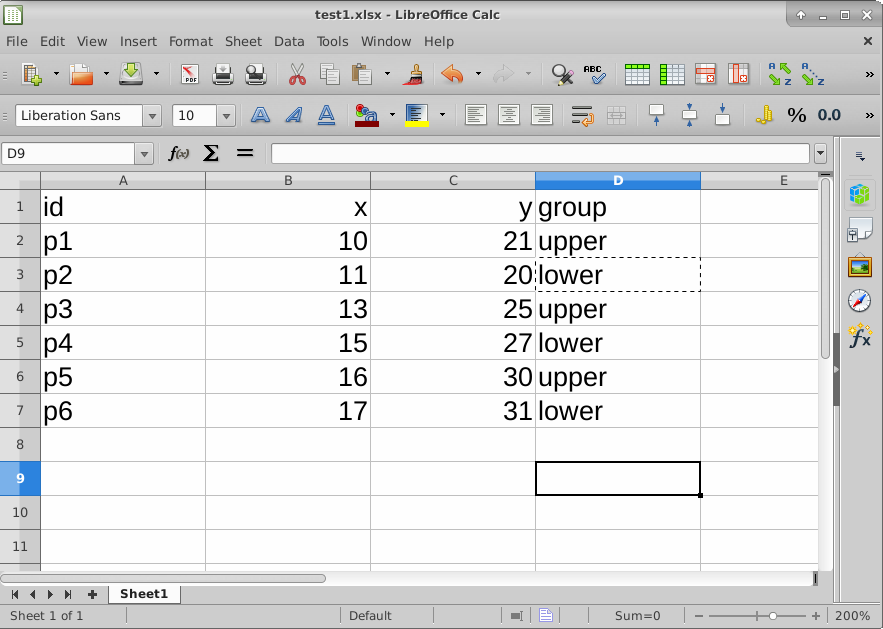
\includegraphics[width=0.9\textwidth]{spreadsheet}
  
\end{frame}

\begin{frame}[fragile]{Save as \texttt{.csv}}
  
  \begin{itemize}
  \item \texttt{.csv} or ``comma-separated values'' is a way of
    turning spreadsheet values into plain text.
  \item but does \emph{not} preserve formulas. (This is a reason for
    doing \emph{all} your calculations in your statistical software,
    and \emph{only} having data in your spreadsheet.)
  \item File, Save As Text CSV (or similar).
  \end{itemize}
  
\end{frame}

\begin{frame}[fragile]{The \texttt{.csv} file}
  
\verbatiminput{test1.csv}
  
\end{frame}


%% \begin{frame}[fragile]{Reading file in R}
%%   
%%   
%%   \begin{itemize}
%%   \item Start (as always) with
%% 
%% <<size="footnotesize",warning=F>>=
%% library(tidyverse)
%% @ 
%% 
%% \item If you don't get this, do this (should only need it once):
%% 
%% <<eval=F>>=
%% install.packages("tidyverse")
%% @ 
%% 
%% 
%% 
%%   \end{itemize}
%%   
%% \end{frame}
%% 
%% \begin{frame}[fragile]{Finding the file}
%%   \begin{itemize}
%% \item Run this:
%%  
%% <<echo=F>>=
%% f="/home/ken/teaching/c32/notes/2017/test1.csv"
%% @   
%% 
%% <<eval=F>>=
%% f=file.choose()
%% @   
%% 
%% This brings up a file selector. Use it to find your \texttt{.csv}
%% file. Then type the name \texttt{f} to display what it contains:
%% 
%% <<>>=
%% f
%% @ 
%% 
%% (This is Linux. Mac looks similar, Windows different.)
%% 
%% \item Now R knows where our file is, and we can read it in (over).
%%   \end{itemize}
%% \end{frame}
%% 
%% \begin{frame}[fragile]{Reading in the file}
%%   
%%   \begin{itemize}
%%   \item Use \texttt{read\_csv} with the name of the file. Save the
%%     read-in file in something, here called \texttt{mydata}: 
%%     
%% <<>>=
%% mydata=read_csv(f)
%% @     
%% \item \texttt{read\_csv} guesses what kind of thing is in each
%%   column. Here it correctly guesses that:
%%   
%%   \begin{itemize}
%%   \item   \texttt{id} and
%%   \texttt{group} are text (categorical variables). \texttt{id} is
%%   actually ``identifier variable'': identifies
%%   individuals. 
%% \item \texttt{x} and \texttt{y} are integers (quantitative variables
%%   that here have no decimal point). Decimal numbers would be labelled
%%   \texttt{num} or \texttt{double}. 
%% 
%%   \end{itemize}
%%   
%% 
%%   \end{itemize}
%%   
%% \end{frame}
%% 
%% \begin{frame}[fragile]{Looking at what we read in}
%%   
%%   \begin{itemize}
%% \item Again, type the name of the thing to display it:
%%   
%% <<>>=
%% mydata
%% @   
%% 
%% \item This is a ``tibble'' or data frame, the standard way of storing
%%   a data set in R.
%% \item Tibbles print as much as will display on the screen. If there
%%   are more rows or columns, it will say so.
%%   \end{itemize}
%%   
%% \end{frame}
%% 
%% \begin{frame}[fragile]{\texttt{View}-ing your data frame}
%%     
%%     \begin{itemize}
%%     \item Another way to examine your data frame is to View it, like this:
%%       
%% <<eval=F>>=
%% View(mydata)
%% @       
%% 
%% \item This pops up a ``data frame viewer'' top left:
%%   
%%   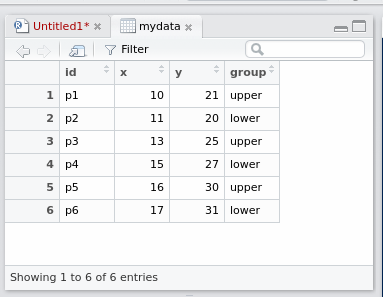
\includegraphics[width=0.6\textwidth]{viewview}
%%     \end{itemize}
%%   
%% \end{frame}
%% 
%% \begin{frame}[fragile]{What you can and cannot do with this View}
%%   
%%   \begin{itemize}
%%   \item Read-only: cannot edit data
%%   \item Can display data satisfying conditions: click on Filter, then:
%%     \begin{itemize}
%%     \item for a categorical variable, type name of category you want
%%     \item for a quantitative variable, use slider to describe values
%%       you want.
%%     \end{itemize}
%%   \item Can sort a column into ascending or descending order (click
%%     little arrows next to column name).
%%     
%%   \item Clicking the symbol with arrow on it left of Filter ``pops
%%     out'' View into separate (bigger) window.
%%   \item Cannot include in output to hand in (except by taking
%%     screenshot and handing \emph{that} in).
%%   \end{itemize}
%%   
%% \end{frame}
%% 
%% \begin{frame}[fragile]{Summarizing what we read in}
%%   
%%   \begin{itemize}
%%   \item It is \emph{always} a good idea to look at your data after you
%%     have read it in, to make sure you have believable numbers (and the
%%     right number of individuals and variables). 
%%   \item Sometimes the data set is too big, and you want to summarize it:
%%     
%% <<>>=
%% glimpse(mydata)
%% @     
%% 
%% \item This tells you how many observations and variables, and shows
%%   you the first few values (almost all of them here).
%%   \end{itemize}
%%   
%% \end{frame}
%% 
%% \begin{frame}[fragile]{Five-number summary}
%%   
%%   \begin{itemize}
%%   \item this way:
%%     
%% <<size="footnotesize">>=
%% summary(mydata)
%% @     
%% 
%% \item For quantitative variables, a five-number summary plus the mean.
%% \item For categorical variables, count of how many rows.
%% \item Quick check for errors: these often show up as values too high
%%   or too low, so the min and/or max will be unreasonable.
%%   \end{itemize}
%%   
%% \end{frame}
%% 
%% \begin{frame}[fragile]{Reading from a URL}
%%   
%%   \begin{itemize}
%%   \item Any data file on the Web can be read directly.
%%   \item Example data:
%%     \url{http://www.utsc.utoronto.ca/~butler/c32/global.csv}.
%%   \item Use URL instead of filename:
%%     
%% <<>>=
%% url="http://www.utsc.utoronto.ca/~butler/c32/global.csv"
%% global=read_csv(url)
%% @     
%%   \end{itemize}
%%   
%% \end{frame}
%% 
%% \begin{frame}[fragile]{The data}
%%   
%% <<>>=
%% global
%% @   
%%   
%% \end{frame}

\begin{frame}[fragile]{Reading files in SAS}
  
  \begin{itemize}
  \item In SAS Studio, click on Files (Home) and find the Upload
    button (4th one in top row) (should be not greyed out):
    

\includegraphics[width=0.5\textwidth]{upload}

  \end{itemize}
  
\end{frame}

\begin{frame}[fragile]{\ldots Continued}
  
  \begin{itemize}
\item Click the Upload button, and then Choose Files in the box that
  pops up. This brings up a file selector as \texttt{file.choose} does
  in R. Find your \texttt{.csv} file, and click to ``open'' it. It
  should appear on your Upload Files box:
  
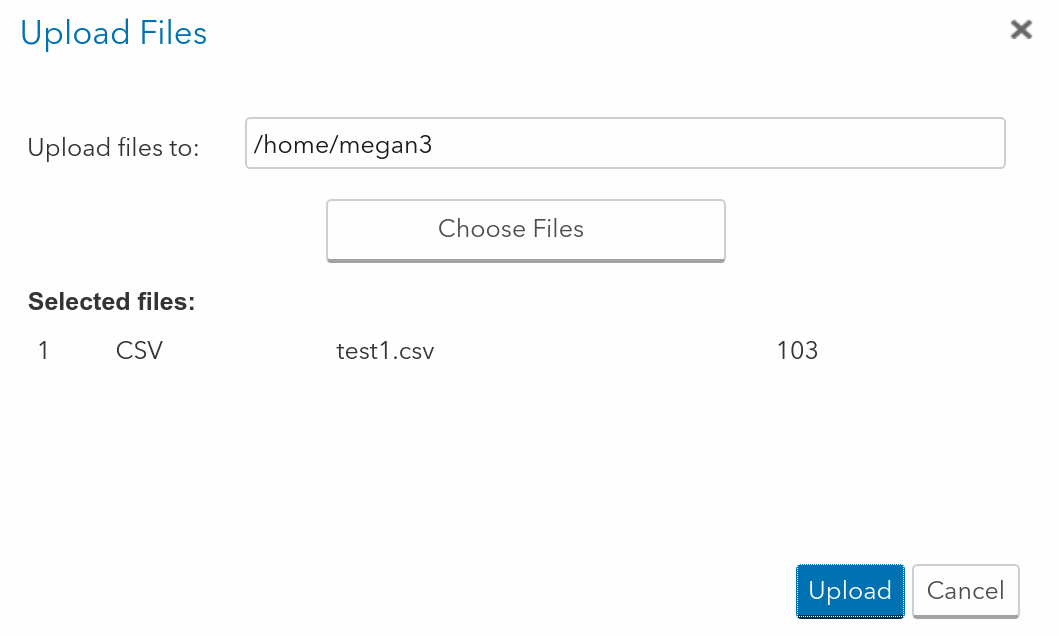
\includegraphics[width=0.5\textwidth]{upload-file}

\item Click Upload. When it's done, you should see your \texttt{.csv}
  file under Files (Home) on the left.
  \end{itemize}
  
\end{frame}

\begin{frame}[fragile]{Reading in the data}
  
  \begin{itemize}
  \item In SAS Studio, click New (leftmost button under Server Files
    and Folders) and select New SAS Program.
  \item On the right, in the Code tab, type code like this, only
    instead of \texttt{ken} put \emph{your} username:
    
\begin{Datastep}
proc import 
  datafile='/home/ken/test1.csv'
  dbms=csv
  out=mydata
  replace;
  getnames=yes;
\end{Datastep}
    
\begin{Sascode}[store=ra]
proc print;
\end{Sascode}
  \item Make sure you get \emph{all} the semicolons in the right
    places!
  \item This will read in the data that you uploaded, and list the
    whole data set. Compare R \texttt{read\_csv}.
  \end{itemize}
  
\end{frame}


\begin{frame}[fragile]{Running the code}
  
  \begin{itemize}
  \item Find the ``running human'' under the word Code. Click it. 
  \item If all goes well, you should see the data set displayed in a
    Results tab:
    
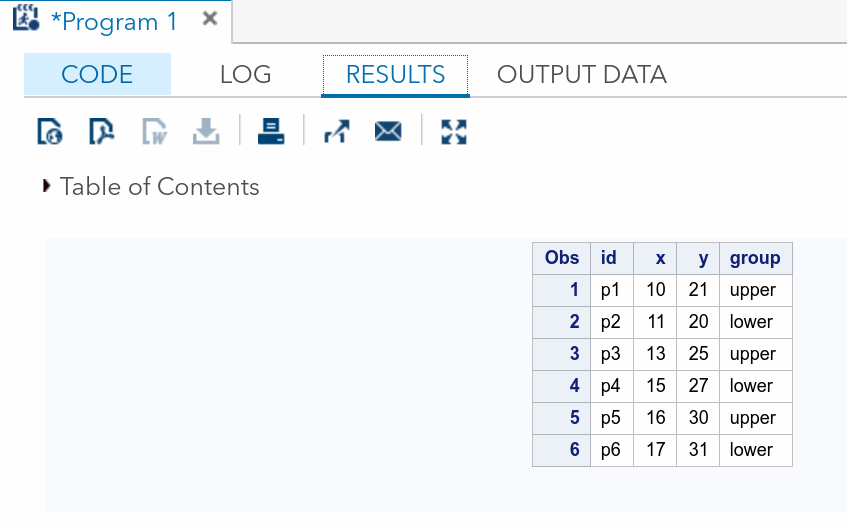
\includegraphics[width=0.7\textwidth]{sasstudio-results}

\item If not, you'll get taken to the Log tab, which will show you
  where your error was. Fix it, and try again. (SAS can sometimes
  guess what you meant, even if it's not what you typed.)
  \end{itemize}
  
\end{frame}

\begin{frame}[fragile]{That code}
  
  \begin{itemize}
  \item \texttt{proc print} displays the whole data set.
  \item The \texttt{proc import} organizes reading in the data. I
    remember DODRG:
    \begin{itemize}
    \item \texttt{datafile} says where to find the data file (on SAS
      Studio's server, where you uploaded it to).
    \item \texttt{out} gives the data set a name within SAS (that can
      be used to refer to this data set later)
    \item \texttt{dbms} says what kind of file it is, a \texttt{.csv}
      in this case.
    \item \texttt{replace} says to replace any other SAS data set on
      your account with this name (the one on \texttt{out}).
    \item \texttt{getnames} means to take the variable names from the
      top line of the data file (which is usually where they are). 
    \end{itemize}
  \end{itemize}
  
\end{frame}

\begin{frame}[fragile]{Alternatively}
  
  \begin{itemize}
  \item Click the New button, but then Import Data.
  \item Find your data file on the left, and drag it across to Select
    File on the right.
  \item Some code will appear. This is (basically) the \texttt{proc
      import} code we used above.
  \item Copy the text from \texttt{FILENAME} down to \texttt{RUN;}
    (inclusive).
  \item Open a New SAS Code window. Paste the copied code into it.
  \item Add anything else at the bottom, like a \texttt{proc print},
    and run as before.
  \end{itemize}
  
\end{frame}

\begin{frame}[fragile]{Summarizing a data set}
  
  \begin{itemize}
  \item Replace the \texttt{proc print} with \texttt{proc means}:
    
    \begin{Sascode}[store=rb]
proc means;      
    \end{Sascode}
    
    That gives the mean, SD, min, max and \#observations for each
    variable (below). Like R \texttt{group\_by}, \texttt{summarize}.
    
    \item Note that you only get means for quantitative variables.
    \item \texttt{proc print}, \texttt{proc means} etc.\ work on
      \emph{the most recently created data set} (usually what you
      want). 
    
\Listing[store=rb,fontsize=scriptsize]{rbb}    


  \end{itemize}
  
\end{frame}

\begin{frame}[fragile]{Reading from a URL}
  
  \begin{itemize}
  \item A little extra setup:
    
    \begin{small}
    \begin{Sascode}[store=ua]
filename myurl url 
  "http://www.utsc.utoronto.ca/~butler/c32/global.csv";

proc import 
  datafile=myurl 
  dbms=csv
  out=global
  replace;
  getnames=yes;
  
proc print;
    \end{Sascode}
      
    \end{small}
    
    
  \item The \texttt{filename} line says that the piece of text is
    actually a URL rather than a filename on this computer.
  \end{itemize}
  
\end{frame}

\begin{frame}[fragile]{Did it work?}
  
\Listing[store=ua,fontsize=footnotesize]{uaa}  
  
\end{frame}

\begin{frame}[fragile]{Space-delimited files}
  
  \begin{itemize}
  \item Another common format for data is a text file with the values
    separated by spaces. Data below in two long columns with right
    side below left side:
    
    \begin{footnotesize}
    \begin{multicols}{2}
\verbatiminput{/home/ken/coffee.txt}      
    \end{multicols}
      
    \end{footnotesize}
    
  \end{itemize}
  
\end{frame}

\begin{frame}[fragile]{Reading in these data}
  
  \begin{itemize}
  \item Change the \texttt{proc import}:
    
    \begin{Datastep}
filename myurl url 
  "http://www.utsc.utoronto.ca/~butler/c32/coffee.txt";      
proc import 
  datafile=myurl
  dbms=dlm
  out=coffee
  replace;
  delimiter=' ';
  getnames=yes;
    \end{Datastep}
  \item On \texttt{dbms}, \texttt{dlm} means ``delimited file'', that
    is, ``values separated by something''. So we have to say what the
    values are separated by, namely exactly one space. (The values
    could be separated by anything.) 
  \item Equivalent to R \texttt{read\_delim}.
  \end{itemize}
  
\end{frame}

\begin{frame}[fragile]{Did it work?}
  
  \begin{itemize}
  \item The first 15 (of 32) lines. It seems to have worked:
    
    \begin{Sascode}[store=rc]
proc print data=coffee(obs=15);      
    \end{Sascode}
    
    \Listing[store=rc,fontsize=footnotesize]{rcc}
  \end{itemize}
  
\end{frame}

%% \begin{frame}[fragile]{Reading the coffee data into R}
%%   
%%   \begin{itemize}
%%   \item Save the text file somewhere and then find it:
%% <<echo=F>>=
%% f="/home/ken/teaching/c32/notes/2017/coffee.txt"
%% @   
%% <<eval=F>>=
%% f=file.choose()
%% @   
%% <<>>=
%% f
%% @
%% \item This time, \texttt{read\_delim}, and again we have to say what
%%   the thing is separating the values:
%%   
%% <<>>=
%% coffee=read_delim(f," ")
%% @   
%% 
%% \item Name of the cup, text, and \texttt{tempdiff}, a decimal number.
%%   \end{itemize}
%%   
%% \end{frame}
%% 
%% \begin{frame}[fragile]{Looking at the values}
%%   
%% <<>>=
%% coffee
%% @   
%% 
%% These were four brands of travel mug (in \texttt{cup}), and for each,
%% how much the temperature of the coffee in the mug decreased over 30
%% minutes. 
%%   
%% \end{frame}
%% 
%% \begin{frame}[fragile]{Reading from the Web}
%%   
%%   \begin{itemize}
%%   \item For R, use the URL in place of the filename (or in place of
%%     the \texttt{f} saved from \texttt{file.choose()}). 
%%   \item for SAS, do the \texttt{filename} thing, which works for any
%%     type of file.
%%   \end{itemize}
%%   
%% \end{frame}
%% 
%% \begin{frame}[fragile]{Reading soap data in R}
%%   
%% <<>>=
%% url="http://www.utsc.utoronto.ca/~butler/c32/soap.txt"
%% soap=read_delim(url," ")
%% @   
%%   
%% \end{frame}
%% 
%% \begin{frame}[fragile]{The soap data}
%%   
%% <<>>=
%% soap
%% @   
%%   
%% \end{frame}

\begin{frame}[fragile]{Reading soap data in SAS}
  
  \begin{Sascode}[store=ub]
filename myurl 
 url 
 "http://www.utsc.utoronto.ca/~butler/c32/soap.txt";

proc import 
  datafile=myurl 
  dbms=dlm
  out=soap
  replace;
  delimiter=' ';
  getnames=yes;
  
proc print data=soap(obs=10);

  \end{Sascode}
  
\end{frame}

\begin{frame}[fragile]{Ten rows of the soap data}
  
\Listing[store=ub,fontsize=footnotesize]{ubb}  
  
\end{frame}

%% \begin{frame}[fragile]{Data aligned in columns}
%%   
%%   \begin{itemize}
%%   \item Sometimes you see data aligned in columns, thus:
%%     
%%     \begin{small}
%% \begin{verbatim}
%% DrugA DrugB DrugC
%%   4     6     6
%%   5     8     7
%%   4     4     6
%%   3     5     6
%%   2     4     7
%%   4     6     5
%%   3     5     6
%%   4     8     5
%%   4     6     5
%% \end{verbatim}      
%%       \item \texttt{read\_delim} \emph{will not} work: values
%%         separated by \emph{more than one} space.
%%       \item In R, \texttt{read\_table} works for this.
%%       \item In SAS, not possible with \texttt{proc import}.
%%     \end{small}
%%   \end{itemize}
%%   
%% \end{frame}
%% 
%% \begin{frame}[fragile]{Reading in column-aligned data}
%%   
%%   \begin{multicols}{2}
%% <<size="small">>=
%% drugs=read_table("migraine.txt")
%% @   
%% 
%% <<>>=
%% drugs
%% @ 
%%     
%%   \end{multicols}
%% 
%% \end{frame}

\begin{frame}[fragile]{Reading an Excel sheet directly}
  
  \begin{itemize}
  \item Here is my spreadsheet from before, but tarted up a bit:

    \begin{center}
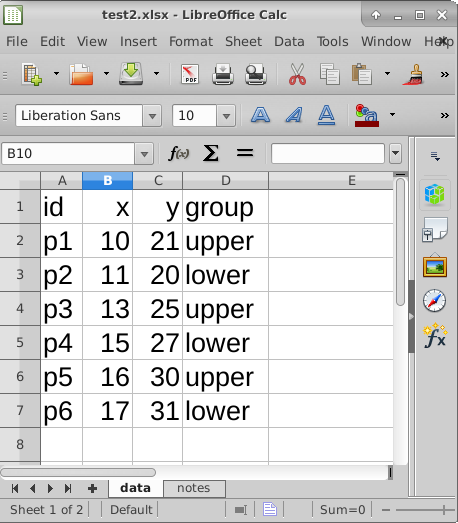
\includegraphics[width=0.4\textwidth]{excel}      
    \end{center}
    
\item It is now a workbook with a second sheet called ``notes'' (that
  we don't want).
  \end{itemize}
  
\end{frame}

%% \begin{frame}[fragile]{Reading it in}
%%   
%%   \begin{itemize}
%% \item Read into R, saying that we only want the sheet ``data''. Start
%%   with \texttt{file.choose} as before (omitted):
%%   
%% <<echo=F>>=
%% f="/home/ken/teaching/c32/notes/2017/test2.xlsx"
%% @   
%% <<>>=
%% library(readxl)
%% mydata2=read_excel(f,sheet="data")
%% mydata2
%% @   
%% \item That has worked properly.
%%   \end{itemize}
%%   
%% \end{frame}

\begin{frame}[fragile]{Reading Excel spreadsheet into SAS}
  
  \begin{itemize}
  \item Upload the spreadsheet file (as for uploading \texttt{.csv}
    file)
  \item Then, like this:
    
    \begin{Datastep}
proc import 
  datafile='/home/ken/test2.xlsx'
  dbms=xlsx
  out=mydata
  replace;
  sheet=data;
  getnames=yes;
    \end{Datastep}
    
    
  \item \texttt{dbms} is now \texttt{xlsx} for reading this type of
    file (or \texttt{xls} if you have old-style spreadsheet).
  \item Use \texttt{sheet=} to say which worksheet you want (no quotes).
    
  \item Equivalent to R \texttt{read\_excel}.
  \end{itemize}
  
\end{frame}

\begin{frame}[fragile]{The spreadsheet as data set}

  
  \begin{itemize}
  \item Did it work? Yes:

    \begin{Sascode}[store=re]
proc print;    
  \end{Sascode}
  
  \Listing[store=re]{ree}


  \end{itemize}
  
  
\end{frame}

\begin{frame}[fragile]{Reading Excel files from the Web}
  
  \begin{itemize}
  \item Recall that R's \texttt{read\_excel} required us to
    download-save spreadsheet first then read it from local file.
  \item SAS has no such requirements here.
  \item Define a \texttt{filename myurl url} as before, and use it in
    the appropriate \texttt{proc import}.
    
  \end{itemize}
  
\end{frame}

% making graphs


\section{Graphs}

\frame{\sectionpage}

\begin{frame}[fragile]{Our data}
  
  \begin{itemize}
  \item Once again use data on 202 male and female athletes at the
    Australian Institute of Sport.
  \item Variables:
    \begin{itemize}
    \item categorical: Sex of athlete, sport they play 
    \item quantitative: height (cm), weight (kg), lean body mass, red
      and white blood cell counts, haematocrit and haemoglobin
      (blood), ferritin concentration, body mass index, percent body
      fat. 
    \end{itemize}
  \item Values separated by \emph{tabs} (which impacts reading in).

  \end{itemize}
  
\end{frame}

%% \begin{frame}[fragile]{Reading data into R}
%%   
%% <<echo=F, message=F>>=
%% require(tidyverse)
%% @   
%%   
%%   \begin{itemize}
%%   \item Use \texttt{read\_tsv} (``tab-separated values''), like
%%     \texttt{read\_csv}.
%%   \item Data in \texttt{ais.txt}:
%%     
%% <<size="small">>=
%% athletes=read_tsv("ais.txt")
%% @  
%% 
%%   \end{itemize}
%%   
%% \end{frame}
%% 
%% \begin{frame}[fragile]{The data (some)}
%%   
%% <<size="footnotesize">>=
%% athletes
%% @   
%%   
%% \end{frame}

\begin{frame}[fragile]{Reading data into SAS}
  
  \begin{itemize}
    \item Upload file to SAS Studio first.
    \item Or get from
      \url{http://www.utsc.utoronto.ca/~butler/c32/ais.txt} and use
      \texttt{filename myurl url} thing first.
      
    \item R equivalent: \texttt{read\_tsv}.
  \item A bit trickier because we can't \emph{type} tab: have to use
    special code \texttt{'09'x} (ASCII code \texttt{09} in hex):
    
    \begin{Datastep}
filename myurl url 
  "http://www.utsc.utoronto.ca/~butler/c32/ais.txt";
proc import 
  datafile=myurl
  dbms=dlm
  out=sports
  replace;
  delimiter='09'x;
  getnames=yes;

    \end{Datastep}
  \end{itemize}
  
\end{frame}

\begin{frame}[fragile]{Some of the data, tiny}
  
  \begin{Sascode}[store=ga]
proc print data=sports(obs=9);
  \end{Sascode}
  
\Listing[fontsize=scriptsize,store=ga]{gaa}  
  
\end{frame}

\begin{frame}[fragile]{Or, summarized}
  
  \begin{Sascode}[store=gb]
proc means;    
  \end{Sascode}
  
\Listing[store=gb,fontsize=scriptsize]{gbb}  
  
\end{frame}

\begin{frame}[fragile]{Kinds of graph}
  
  Reminder: depends on number and type of variables you have:
  
  \begin{center}
  \begin{tabular}{ccp{0.3\textwidth}p{0.35\textwidth}}
    Categ.\ & Quant.\ & Graph & R equiv.\ \\
    \hline
    1 & 0 & bar chart & \texttt{geom\_bar}\\
    0 & 1 & histogram & \texttt{geom\_histogram}\\
    2 & 0 & grouped bar charts & \texttt{geom\_bar}, \texttt{fill}\\
    1 & 1 & side-by-side boxplots & \texttt{geom\_boxplot}\\
    0 & 2 & scatterplot & \texttt{geom\_point} \\
    2 & 1 & grouped boxplots & \texttt{geom\_boxplot}, \texttt{colour}\\
    1 & 2 & scatterplot with points identified by group (eg.\ by
            colour) & \texttt{geom\_point}, \texttt{colour}\\
    \hline
  \end{tabular}
    
  \end{center}
  
  With more variables, \emph{separate plots by groups}:
  \texttt{paneling} in SAS (\texttt{facetting} in R).
  
\end{frame}

\begin{frame}[fragile]{Workhorse graphing procedure}
  
  \begin{itemize}
  \item   SAS also has standard graphing procedure, that we use for all our
  SAS graphs. 
  \item \textbf{proc sgplot}
  \item   Use in different ways to get precise graph we want.
\item   Start with bar chart of the sports played by the athletes.

  \end{itemize}
    
  
\end{frame}

%% \begin{frame}[fragile]{Bar chart in R}
%%   
%% <<fig.height=4>>=
%% ggplot(athletes,aes(x=Sport))+geom_bar()
%% @   
%%   
%% \end{frame}

\begin{frame}[fragile]{Bar chart in SAS}
  
  \begin{Sascode}[store=gd]
proc sgplot;
  vbar Sport;
  \end{Sascode}
  
  \Graphic[store=gd,scale=0.5]{gdd}
  
\end{frame}

\begin{frame}[fragile]{Histogram of body mass index, in SAS}
  
  \begin{Sascode}[store=ge]
proc sgplot;
  histogram BMI;
  \end{Sascode}
  
  \Graphic[store=ge,scale=0.5]{gee}

  
\end{frame}

%% \begin{frame}[fragile]{BMI histogram in R}
%%   
%% <<fig.height=4>>=
%% ggplot(athletes,aes(x=BMI))+geom_histogram(bins=10)
%% @   
%%   
%% \end{frame}
%% \begin{frame}[fragile]{Which sports are played by males and females?}
%%   
%% 
%%   
%% <<fig.height=3.5>>=
%% ggplot(athletes,aes(x=Sport,fill=Sex))+
%%   geom_bar(position="dodge")
%% @   
%%   
%% \end{frame}

\begin{frame}[fragile]{Grouped bar plot in SAS}
  
  \begin{Sascode}[store=gf]
proc sgplot;
  vbar Sport / group=Sex groupdisplay=cluster;
  \end{Sascode}
  
  \Graphic[store=gf,scale=0.5]{gff}
  
\end{frame}

\begin{frame}[fragile]{BMI by gender}
  
  Side-by-side boxplots:
  
  \begin{Sascode}[store=gg]
proc sgplot;
  vbox BMI / category=Sex;
  \end{Sascode}
  
  \Graphic[store=gg,scale=0.5]{ggg}
  
\end{frame}

%% \begin{frame}[fragile]{And in R}
%% <<fig.height=4>>=
%% ggplot(athletes,aes(x=Sex,y=BMI))+geom_boxplot()
%% @   
%% \end{frame}
%% 
%% \begin{frame}[fragile]{Height vs.\ weight}
%%   
%%   Scatterplot:
%%   
%% <<fig.height=4>>=
%% ggplot(athletes,aes(x=Ht,y=Wt))+geom_point()
%% @   
%%   
%% \end{frame}

\begin{frame}[fragile]{Height vs.\ weight}
  
  \begin{Sascode}[store=gh]
proc sgplot;
  scatter x=Ht y=Wt;
  \end{Sascode}
  
  \Graphic[store=gh,scale=0.5]{ghh}
  
\end{frame}

\begin{frame}[fragile]{and again, with regression line}
  
  \begin{Sascode}[store=gj]
proc sgplot;
  scatter x=Ht y=Wt;
  reg x=Ht y=Wt;
  \end{Sascode}
  
  \Graphic[store=gj,scale=0.5]{gjj}
  
  
\end{frame}

%% \begin{frame}[fragile]{One more time}
%%   
%% <<fig.height=4>>=
%% ggplot(athletes,aes(x=Ht,y=Wt))+
%%   geom_point()+geom_smooth(method="lm")
%% @   
%%   
%% \end{frame}

\begin{frame}[fragile]{BMI by sport and gender}
  
  \begin{Sascode}[store=gi]
proc sgplot;
  vbox BMI / group=Sex category=Sport;
  \end{Sascode}
  
  \Graphic[store=gi,scale=0.5]{gii}
\end{frame}

%% \begin{frame}[fragile]{R}
%%   
%% <<fig.height=4>>=
%% ggplot(athletes,aes(x=Sport,y=BMI,colour=Sex))+
%%   geom_boxplot()
%% @   
%%   
%% \end{frame}
%% 
%% \begin{frame}[fragile]{Height and weight by gender}
%% 
%% <<fig.height=4>>=
%% ggplot(athletes,aes(x=Ht,y=Wt,colour=Sex))+
%%   geom_point()
%% @   
%%   
%% \end{frame}

\begin{frame}[fragile]{Scatterplot by gender}
  
  \begin{Sascode}[store=gk]
proc sgplot;
  scatter x=Ht y=Wt / group=Sex;
  \end{Sascode}
  
  \Graphic[store=gk,scale=0.5]{gkk}
  
\end{frame}

\begin{frame}[fragile]{Height by weight for each sport}
  
  Separate plot for each sport, first two panels here:
  
  \begin{Sascode}[store=gl]
proc sgpanel;
  panelby Sport;
  scatter x=Ht y=Wt / group=Sex;
  \end{Sascode}
  
  \Graphic[store=gl,scale=0.5]{gll}
  
  
\end{frame}

%% \begin{frame}[fragile]{same in R, with facets}
%%   
%% <<fig.height=4>>=
%% ggplot(athletes,aes(x=Ht,y=Wt,colour=Sex))+
%%   geom_point()+facet_wrap(~Sport)
%% @   
%%   
%%   
%% \end{frame}
%% 
%% \begin{frame}[fragile]{Filling each facet}
%%   
%%   Default uses same scale for each facet. To use different scales for
%%   each facet, this:
%%   
%% <<fig.height=3.5>>=
%% ggplot(athletes,aes(x=Ht,y=Wt,colour=Sex))+
%%   geom_point()+facet_wrap(~Sport,scales="free")
%% @   
%%   
%%   
%% \end{frame}


% numerical summaries


\section{More detailed summaries of data}

\frame{\sectionpage}

%% \begin{frame}[fragile]{Summarizing data in R}
%% 
%% <<results="hide",echo=F,message=F>>=
%% require(tidyverse)
%% @   
%%   
%%   \begin{itemize}
%%   \item 
%%     What if we want:
%%     
%%     \begin{itemize}
%%     \item a summary or two of just one column
%%     \item a count of observations in each category of a categorical
%%       variable? 
%%     \item summaries by group
%%     \item a different summary of all columns (eg.\ SD)
%%     \end{itemize}
%%     
%%   \item To do this, meet \textbf{pipe} operator \texttt{\%>\%}. This
%%     takes input data frame, does something do it, and outputs result.
%%   \item Output from a pipe can be used as input to something else, so
%%     can have a sequence of pipes.
%%   \item Summaries include: \texttt{mean}, \texttt{median},
%%     \texttt{min}, \texttt{max},
%%     \texttt{sd}, \texttt{IQR}, \texttt{quantile} (for obtaining
%%     quartiles or any percentile), \texttt{n} (for counting
%%     observations). 
%%   \item Use our Australian athletes data again.
%%   \end{itemize}
%%   
%% \end{frame}
%% 
%% \begin{frame}[fragile]{Summarizing one column}
%%   \begin{itemize}
%%   \item Like this, for example the mean height:
%%     
%% <<>>=
%% athletes %>% summarize(m=mean(Ht))
%% @     
%% 
%% or to get mean and SD of BMI:
%% 
%% <<>>=
%% athletes %>% summarize(m=mean(BMI),s=sd(BMI))
%% @ 
%%   \end{itemize}
%% \end{frame}
%% 
%% \begin{frame}[fragile]{Quartiles}
%%   
%%   \begin{itemize}
%%   \item \texttt{quantile} calculates percentiles, so we want the 25th
%%     and 75th percentiles:
%%     
%% <<>>=
%% athletes %>% summarize( Q1=quantile(Wt,0.25),
%%                         Q3=quantile(Wt,0.75))
%% @     
%%   \end{itemize}
%%   
%% \end{frame}
%% 
%% \begin{frame}[fragile]{Counting how many}
%%   
%%   \begin{multicols}{2}
%%   for example, number of athletes in each sport:
%%   
%% <<>>=
%% athletes %>% count(Sport)
%% @   
%%   
%% Another way (which will make sense in a moment):
%% 
%% <<size="small">>=
%% athletes %>% group_by(Sport) %>% 
%%   summarize(count=n())
%% @ 
%%     
%%   \end{multicols}
%%   
%% \end{frame}
%% 
%% \begin{frame}[fragile]{Summaries by group}
%%   
%%   \begin{itemize}
%%   \item Might want separate summaries for each ``group'', eg.\ mean
%%     and SD of height for males and females. Strategy is
%%     \texttt{group\_by} (to define the groups) and then \texttt{summarize}:
%%     
%% <<>>=
%% athletes %>% group_by(Sex) %>%
%%   summarize(m=mean(Ht),s=sd(Ht))
%% @     
%% 
%% \item This explains second variation on counting within group:
%%   ``within each sport, how many athletes were there?''
%%   \end{itemize}
%%   
%% \end{frame}
%% 
%% \begin{frame}[fragile]{Summarizing several columns}
%%   
%%   \begin{itemize}
%%   \item Standard deviation of each (numeric) column:
%%     
%% <<size="footnotesize">>=
%% athletes %>% summarize_if(is.numeric,funs(sd))
%% @   
%% 
%% \item Median and IQR of all columns whose name starts with H:
%%   
%% <<>>=
%% athletes %>% summarize_at(vars(starts_with("H")),
%%   funs(median,IQR))
%% @   
%%       
%%   \end{itemize}
%%   
%% 
%%   
%% \end{frame}




\begin{frame}[fragile]{Summarizing data in SAS}
  
  \begin{itemize}
  \item Already saw \texttt{proc means} to find means, SDs and sample
    sizes.
  \item \texttt{proc means} will also calculate means of only some
    variables or by group.
  \item Also, \texttt{proc means} can calculate other statistics (by
    group if desired), despite its name.
  \item SAS names for other statistics: \texttt{mean},
    \texttt{median}, \texttt{stddev} (SD), \texttt{qrange} (IQR),
    \texttt{Q1}, \texttt{Q3} (quartiles).
  \item R equivalent: (\texttt{group\_by}), \texttt{summarize}
  \end{itemize}
  
\end{frame}

\begin{frame}[fragile]{Specifying summaries, variables and groups}
  
  \begin{itemize}
  \item To specify which summaries to calculate, list them on the
    \texttt{proc means} line.
  \item To specify which variables to calculate summaries for, use a
    line starting with \texttt{var}.
  \item To specify which groups to calculate for, use a line starting
    with \texttt{class} and the name of the grouping variable.
  \item Examples over.

    \begin{Datastep}[program]
data ath;
  set sports;
      \end{Datastep}
    
  \end{itemize}
  
\end{frame}

\begin{frame}[fragile]{Quartiles of athlete weight}
  
  \begin{Sascode}[store=sa]
proc means Q1 Q3 Qrange;
  var Wt;
  \end{Sascode}
  
  \Listing[store=sa,fontsize=small]{saa}
  
\end{frame}

\begin{frame}[fragile]{Mean and SD of height by gender}
  
  \begin{itemize}
  \item Thus:
    
    \begin{Sascode}[store=sb]
proc means mean stddev;
  var Ht;
  class Sex;
    \end{Sascode}
    
    \Listing[store=sb,fontsize=footnotesize]{sbb}
  \end{itemize}
  
\end{frame}

\begin{frame}[fragile]{How many athletes from each sport?}
  
  \begin{itemize}
  \item Have to pick a variable to count observations of (though it
    doesn't matter):
    
    \begin{Sascode}[store=sc]
proc means n;
  var BMI;
  class Sport;
    \end{Sascode}
  \item Results over.
    
  \end{itemize}
  
\end{frame}

\begin{frame}[fragile]{Results}
  
    \Listing[fontsize=scriptsize,store=sc]{scc}
  
  
\end{frame}

\begin{frame}[fragile]{A perhaps better way to count}
  
  \begin{Sascode}[store=sd]
proc freq;
  tables Sport;
  \end{Sascode}
  
  \Listing[fontsize=footnotesize,store=sd]{sdd}
  
\end{frame}


\begin{frame}[fragile]{SD of all the (numerical) columns}
  
  \begin{itemize}
  \item Just don't specify a \texttt{var} or a \texttt{class}:
    
    \begin{Sascode}[store=se]
proc means stddev;
    \end{Sascode}
    
    \Listing[store=se]{see}
  \end{itemize}
  
\end{frame}


% statistical inference


\section{Inference}

\frame{\sectionpage}


%% \begin{frame}{Statistical Inference and Science}
%% 
%% <<results="hide",echo=F,message=F>>=
%% require(tidyverse)
%% @   
%% 
%% \begin{itemize}
%% \item Previously: \emph{descriptive statistics}. ``Here are data; what
%%   do they say?''.
%% \item May need to \emph{take some action} based on information in data.
%% \item Or want to \emph{generalize} beyond data (sample) to larger
%%   world (population).
%% \item Science: first guess about how world works.
%% \item Then collect data, by sampling.
%% \item Is guess correct (based on data) for whole world, or not?
%% \end{itemize}
%% 
%% \end{frame}
%% 
%% \begin{frame}[fragile]{Sample data are imperfect}
%%   
%%   \begin{itemize}
%%   \item Sample data never entirely represent what you're observing.
%%   \item There is always random error present.
%%   \item Thus you can never be entirely certain about your conclusions.
%%   \item The Toronto Blue Jays' average home attendance in part of 2015
%%     season was 25,070
%%     (up to May 27 2015, from \url{baseball-reference.com}).
%%   \item Does that mean the attendance at every game was exactly
%%     25,070? Certainly not. Actual attendance depends on many things, eg.:
%%     \begin{itemize}
%%     \item how well the Jays are playing
%%     \item the opposition
%%     \item day of week
%%     \item weather
%%     \item random chance
%%     \end{itemize}
%%   \end{itemize}
%%   
%% \end{frame}
%% 
%% \begin{frame}[fragile]{Reading the attendances}
%% 
%% \ldots as a \texttt{.csv} file:
%% 
%% <<>>=
%% jays=read_csv("jays15-home.csv")
%% @   
%%   
%% \end{frame}
%% 
%% \begin{frame}[fragile]{Taking a look}
%%   
%% <<size="footnotesize">>=
%% jays
%% @   
%%   
%% \end{frame}
%% 
%% \begin{frame}[fragile]{Another way}
%% <<size="scriptsize">>=
%% glimpse(jays)
%% @   
%% \end{frame}
%% 
%% \begin{frame}[fragile]{Attendance histogram}
%% <<fig.height=4>>=
%% ggplot(jays,aes(x=attendance))+geom_histogram(bins=10)
%% @   
%% 
%% \end{frame}
%% 
%% \begin{frame}[fragile]{Comments}
%%   
%%   \begin{itemize}
%%   \item Attendances have substantial variability, ranging from just
%%     over 10,000 to around 50,000.
%%   \item Distribution somewhat skewed to right (but no outliers).
%%   \item These are a sample of ``all possible games'' (or maybe ``all
%%     possible games played in April and May''). What can we say about
%%     mean attendance in all possible games based on this evidence?
%%   \item Think about:
%%     \begin{itemize}
%%     \item Confidence interval
%%     \item Hypothesis test.
%%     \end{itemize}
%%   \end{itemize}
%%   
%% \end{frame}
%% 
%% 
%% 
%% \begin{frame}[fragile]{Getting CI for mean attendance}
%%   
%%   \begin{itemize}
%%   \item \texttt{t.test} function does CI and test. Look at CI first:
%% <<>>=
%% t.test(jays$attendance)  
%% @ 
%% \item From 20,500 to 29,600.
%% 
%%   \end{itemize}
%%   
%% \end{frame}
%% 
%% \begin{frame}[fragile]{Or, 90\% CI}
%%   
%%   \begin{itemize}
%%   \item by including a value for \texttt{conf.level}:
%% <<>>=
%% t.test(jays$attendance,conf.level=0.90)  
%% @ 
%% \item From 21,300 to 28,800. (Shorter, as it should be.)
%%   \end{itemize}
%%   
%% \end{frame}
%% \begin{frame}[fragile]{Comments}
%%   
%%   \begin{itemize}
%%   \item Need to say ``column \texttt{attendance} within data frame
%%     \texttt{jays}'' using \texttt{\$}.
%%   \item 95\% CI from about 20,000 to about 30,000.
%%   \item Not estimating mean  attendance well at all!
%%   \item Generally want confidence interval to be \emph{shorter}, which
%%     happens if:
%%     \begin{itemize}
%%     \item SD smaller
%%     \item sample size \emph{bigger}
%%     \item confidence level smaller
%%     \end{itemize}
%%   \item Last one is a cheat, really, since reducing confidence level
%%     increases chance that interval won't contain pop.\ mean at all!
%%   \end{itemize}
%%   
%% \end{frame}
%% 
%% \begin{frame}[fragile]{Another way to access data frame columns}
%%   
%% <<>>=
%% with(jays,t.test(attendance))
%% @   
%%   
%% \end{frame}
%% 
%% \begin{frame}[fragile]{Hypothesis test}
%%   
%%   \begin{itemize}
%%   \item CI answers question ``what is the mean?''
%%   \item Might have a value $\mu$ in mind for the mean, and question
%%     ``Is the mean equal to $\mu$, or not?''
%%   \item For example, 2014 average attendance was 29,327. 
%%   \item Second question answered by \textbf{hypothesis test}.
%%   \item Value being assessed goes in \textbf{null hypothesis}: here,
%%     $H_0: \mu=29,327$.
%%   \item \textbf{Alternative hypothesis} says how null might be wrong,
%%     eg.\ $H_a: \mu \ne 29,327$.
%%   \item Assess evidence \emph{against null}. If that evidence strong
%%     enough, \emph{reject null hypothesis}; if not, \emph{fail to
%%       reject null hypothesis} (sometimes \emph{retain null}). 
%%   \item Note asymmetry between null and alternative, and utter absence
%%     of word ``accept''. 
%%   \end{itemize}
%%   
%% \end{frame}
%% 
%% \begin{frame}[fragile]{$\alpha$ and errors}
%%   
%%   \begin{itemize}
%%   \item Hypothesis test ends with \emph{decision}:
%%     \begin{itemize}
%%     \item reject null hypothesis
%%     \item do not reject null hypothesis.
%%     \end{itemize}
%%   \item but decision may be \emph{wrong}:
%%     
%% 
%% \begin{center}
%%   
%%   
%% \begin{tabular}{|l|cc|}
%% \hline
%%   & \multicolumn{2}{c|}{Decision}\\
%% Truth & Do not reject & Reject null\\
%% \hline
%% Null true & Correct & Type I error\\
%% Null false & Type II error & Correct\\
%% \hline
%% \end{tabular}
%% \end{center}
%% 
%% \item Either type of error is bad, but for now focus on controlling
%%   Type I error: write $\alpha=P(\mbox{type I error})$, and devise test
%%   so that $\alpha$ \emph{small}, typically 0.05.
%% \item That is, \textbf{if null hypothesis true}, have only small
%%   chance to reject it (which would be a mistake).
%% \item Worry about type II errors later (when we consider power of
%%   test). 
%% 
%%   \end{itemize}
%%   
%% \end{frame}
%% 
%% \begin{frame}[fragile]{Why 0.05? This man.}
%%   
%%   \begin{multicols}{2}
%%   
%%   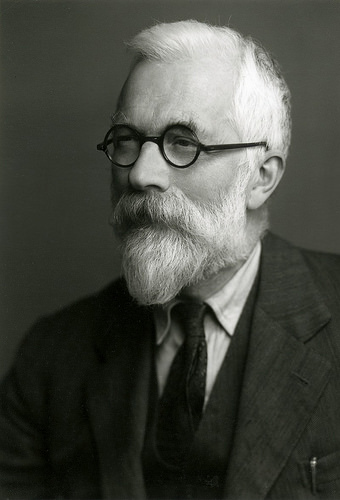
\includegraphics[width=2in]{fisher}
%%   
%%   Responsible for:
%%   
%%   \begin{itemize}
%%   \item analysis of variance
%%   \item Fisher information
%%   \item Linear discriminant analysis
%%   \item Fisher's $z$-transformation
%%   \item Fisher-Yates shuffle
%%   \item Behrens-Fisher problem
%%   \end{itemize}
%% 
%%   Sir Ronald A.\ Fisher, 1890--1962.
%%   \end{multicols}
%%   
%% \end{frame}
%% 
%% \begin{frame}[fragile]{Why 0.05? (2)}
%%   
%%   \begin{itemize}
%%   \item From \emph{The Arrangement of Field Experiments}
%%     (1926):
%%     
%%     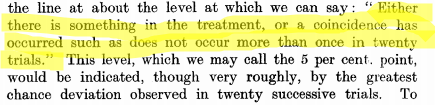
\includegraphics[width=0.9\textwidth]{fisher1}
%%     
%%   \item and
%%     
%%     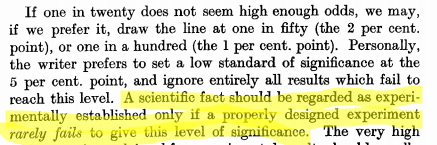
\includegraphics[width=0.9\textwidth]{fisher2}
%%   \end{itemize}
%%   
%% \end{frame}
%% 
%% \begin{frame}[fragile]{Test statistic: going from data to decision}
%%   
%%   \begin{itemize}
%%   \item ``How far away from null hypothesis is data?''
%%   \item In testing for mean, statistic is
%%     $$ t = { \bar{x} - \mu \over s/\sqrt{n} }$$
%%   \item and for our baseball attendance data
%% <<>>=
%% t.stat=(25070-29327)/(11000/sqrt(25)) 
%% t.stat  
%% @ 
%% 
%%   \end{itemize}
%%   
%% \end{frame}
%% 
%% \begin{frame}[fragile]{P-value}
%%   
%%   \begin{itemize}
%%   \item The probability of observing a test statistic value \emph{as
%%       extreme or more extreme than that observed, if the null
%%       hypothesis is true}.
%%   \item ``More extreme'' depends on $H_a$: count both sides if
%%     two-sided, count only the proper side if one-sided.
%%   \item Our $H_a$ was $H_a:  \mu \ne 29,327$, two-sided.
%%   \end{itemize}
%%   
%% \end{frame}
%% 
%% 
%% \begin{frame}[fragile]{$t$-table}
%%   
%%   \begin{multicols}{2}
%% 
%%       \includegraphics[height=0.95\textheight]{StudentTTable}
%% 
%%       \begin{itemize}
%%       \item $n=25$ so df is $25-1=24$.
%%       \item Look up 1.935 not $-1.935$.
%%       \item $1.71 < 1.935 < 2.06$
%%       \item P-value between 0.05 and 0.10
%% 
%% \item P-value not less than 0.05: do not reject null.
%% \item No evidence of change in mean attendance.
%%       \end{itemize}
%%     
%%   \end{multicols}
%%   
%%   
%% \end{frame}
%% 
%% 
%% \begin{frame}[fragile]{Or, again, using \texttt{t.test}:}
%%   
%% <<>>=
%% t.test(jays$attendance, mu=29327)    
%% @ 
%% 
%%   
%%   \begin{itemize}
%%   \item See test statistic $-1.93$, P-value 0.065.
%%   \item Again, do not reject null: conclusion same.
%%   \end{itemize}
%%   
%% \end{frame}
%% 
%% 
\begin{frame}[fragile]{Inference in SAS}
  
  Blue Jays data again:
  
  \begin{Datastep}
filename myurl url 
  "http://www.utsc.utoronto.ca/~butler/c32/jays15-home.csv";
proc import
  datafile=myurl
    dbms=csv
    out=jays
    replace;
  getnames=yes;
  \end{Datastep}
  
\end{frame}

\begin{frame}[fragile]{Checking what I read in}
  
  \begin{itemize}
  \item Especially important in SAS:
    
    \begin{Sascode}[store=iza]
proc print data=jays(obs=6);      
    \end{Sascode}
    
    \Listing[fontsize=tiny,store=iza]{izaa}
  \end{itemize}
  
\end{frame}

\begin{frame}[fragile]{Doing a $t$-test}
  
  of a difference from last year's attendance. Null mean is previous
  year's mean attendance. R: \texttt{t.test}:
  
  \begin{Sascode}[store=ia]
proc ttest h0=29327;
  var attendance;
  \end{Sascode}

  \Listing[store=ia,fontsize=small]{iaa}
  
  Same CI (20527 to 29614) as R, also same P-value 0.0650.

\end{frame}



\begin{frame}[fragile]{Day and night games}
  
  \begin{itemize}
  \item \texttt{daynight} is \texttt{D} for a day game and \texttt{N} for
    a night game. How do attendances compare for these?
\begin{Sascode}[store=id]
  proc sgplot;
    vbox attendance / category=daynight;
\end{Sascode}
  \end{itemize}
  
\end{frame}

\begin{frame}[fragile]{The boxplot}
  
\Graphic[scale=0.5,store=id]{idd}
  
\end{frame}


\begin{frame}[fragile]{Comments}
  
  \begin{itemize}
  \item Attendances on average \emph{much} higher for day games than
    night ones. Why?
  \item We should be cautious about doing a $t$-test here. Why?
  \item What is that upper outlier in the night games?
  \end{itemize}
  
\end{frame}

%\begin{frame}[fragile]{Inference for proportions}
%  
%  \begin{itemize}
%  \item An instant coffee company took a random sample of 100 married
%    men, and found that 20 of the men in the sample preferred that
%    brand of coffee. What can we say about the proportion of all
%    married men that would prefer that brand of coffee?
%    
%  \item Also, is there evidence that the proportion of all married men
%    preferring that brand is greater than 0.15?
%    
%  \item \texttt{prop.test}.
%  
%  \end{itemize}
%  
%\end{frame}
%
%
%\begin{frame}[fragile]{Confidence interval}
%
%\begin{Rcode}
%prop.test(20,100)  
%\end{Rcode}
%
%0.13 to 0.29. Ignore P-value.
%  
%\end{frame}
%
%\begin{frame}[fragile]{and then test}
%
%\begin{Rcode}
%prop.test(20,100,p=0.15,alternative="greater")  
%\end{Rcode}
%
%P-value $0.1038>0.05$, no evidence that proportion greater than
%0.15. (Sample proportion would have to be much bigger, or sample size larger.)
%
%Ignore CI (``one-sided CI''). 
%  
%\end{frame}


\begin{frame}{Another example: learning to read}

  \begin{itemize}
  \item You devised new method for teaching children to read.
  \item Guess it will be more effective than current methods.
  \item To support this guess, collect data.
  \item Want to generalize to ``all children in Canada''.
  \item So take random sample of all children in Canada.
  \item Or, argue that sample you actually have is ``typical'' of all
    children in Canada.
  \item Randomization: whether or not a child in sample or not has
    nothing to do with anything else about that child.
  \item Aside: if your new method good for 
    teaching \emph{struggling} children to read, then ``all
    kids'' is ``all kids having trouble learning to
    read'', and you take a sample of \emph{those}.
  \end{itemize}
  
\end{frame}

\begin{frame}[fragile]{The data, in SAS}

  \begin{itemize}
    \item Data in file \texttt{drp.txt} with header line, group then
    reading test score, separated by \emph{space}:
  \end{itemize}

\begin{Datastep}
filename myurl url 
  "http://www.utsc.utoronto.ca/~butler/c32/drp.txt";  
proc import
  datafile=myurl
  dbms=dlm
  out=reading
  replace;
  delimiter=' ';
  getnames=yes;
\end{Datastep}
%$ %$
\begin{Sascode}[store=ix]
  proc print;
\end{Sascode}
  
\end{frame}


\begin{frame}[fragile]{The data, some, tiny}

  \Listing[store=ix,fontsize=tiny]{ixx}
  
\end{frame}


\begin{frame}[fragile]{Analysis}

  \begin{itemize}
    \item Groups labelled \texttt{c} for ``control'' and \texttt{t}
      for ``treatment''.
    \item Start with summaries (group means) and plot (boxplot).
  \item No pairing, matching: might compare means with \emph{two-sample $t$-test}.
  \item For test, need approx.\ normality, but don't need equal variability.
    \item Use summaries to decide if test reasonable.

  \end{itemize}
  
\end{frame}

\begin{frame}[fragile]{Comparing means}

\begin{Sascode}[store=if]
  proc means;
    class group;
    var score;
\end{Sascode}

\Listing[store=if,fontsize=scriptsize]{iff}
  
\end{frame}

\begin{frame}[fragile]{Boxplots}

\begin{Sascode}[store=ifx]
  proc sgplot;
    vbox score / category=group;
\end{Sascode}

\Graphic[store=ifx,scale=0.5]{ifxx}

  
\end{frame}

\begin{frame}{Comments}

\begin{itemize}
\item Groups not actually same size (maybe 2 kids had to drop out).
\item Means a fair bit different, treatment mean higher.
\item But a lot of variability, so groups do overlap.
\item Standard deviations somewhat different too.
  \item Biggest threat to normality is outliers, none here.
  \item Both distributions not far off symmetric.
  \item $t$-test should be good enough.
  \end{itemize}
  
\end{frame}

\begin{frame}[fragile]{The $t$-test}

  In R, was \texttt{t.test(score\mytilde group)}:
  
\begin{Sascode}[store=ihy]
  proc ttest side=L;
    var score;
    class group;
\end{Sascode}

\Listing[store=ihy,objects=ttests,fontsize=small]{ihyy}

plus a lot more output. 



\end{frame}

\begin{frame}{Comments and Conclusions}

  \begin{itemize}
  \item One-sided test (looking for \emph{improvement}). \texttt{side}
    can be \texttt{L} (lower), \texttt{U} (upper) or \texttt{2}
    (two-sided, can be omitted.) This is \texttt{L} because control
    group first in alphabetical order.
  \item Right $t$-test is Satterthwaite (does not assume equal variability)
  \item P-value $0.0132<0.05$: there \emph{is} increase in reading scores.
  \item Should not use pooled test, because SDs not close; even so,
    result very similar (P-value 0.0143).
  \item One-sided test doesn't give (regular) CI for difference in
    means. To get that, repeat analysis without \texttt{side=L}.
  \end{itemize}
  
\end{frame}

%% \begin{frame}[fragile]{Doing it with R}
%% 
%%   \begin{itemize}
%%   \item Proper reading-in function is \texttt{read\_delim}.
%%   \item If you know that the file is in current folder, read it in by
%%     name (instead of searching for it):
%%     
%% <<>>=
%% kids=read_delim("drp.txt"," ")
%% @     
%% 
%% 
%%   \end{itemize}
%%   
%% \end{frame}
%% 
%% 
%% \begin{frame}[fragile]{The data}
%%   
%% <<size="small">>=
%% kids
%% @   
%%   
%% \end{frame}
%% 
%% \begin{frame}[fragile]{Boxplots}
%%   
%% <<fig.height=4>>=
%% ggplot(kids,aes(x=group,y=score))+geom_boxplot()
%% @   
%%   
%% \end{frame}
%% 
%% \begin{frame}[fragile]{The (Satterthwaite-Welch) $t$-test}
%%   
%%   \begin{itemize}
%%   \item \texttt{c} (control) before \texttt{t} (treatment)
%%     alphabetically, so proper alternative is ``less''.
%%   \item R does Satterthwaite test by default (as before: new reading program really helps):
%% 
%% 
%% <<size="footnotesize">>=
%% t.test(score~group,data=kids,alternative="less")
%% @     
%%   \end{itemize}
%%   
%% \end{frame}
%% 
%% \begin{frame}[fragile]{The pooled $t$-test}
%% 
%%   \begin{itemize}
%%   \item Pooled (equal variances) test this way:
%% 
%% <<>>=
%% t.test(score~group,data=kids,alternative="less",
%%   var.equal=T)
%% @ 
%% 
%% \item Similar P-value to Satterthwaite test (and same results as SAS).
%%   \end{itemize}
%%   
%% \end{frame}
%% 
%% \begin{frame}[fragile]{Two-sided test; CI}
%%   
%%   \begin{itemize}
%% \item To do 2-sided test, leave out \texttt{alternative}:
%% 
%%   {\small
%% <<>>=
%% t.test(score~group,data=kids)
%% @ 
%% }
%% 
%% \item Also gives CI: new reading program increases average scores by somewhere
%%   between about 1 and 19 points. 
%% \item Confidence intervals inherently two-sided, so do 2-sided test to
%%   get them.
%% 
%%   \end{itemize}
%% 
%% \end{frame}
%% 
%% %\begin{frame}{Jargon for testing}
%% %
%% %  \begin{description}
%% %  \item[Alternative hypothesis:] what we are trying to prove (new reading
%% %    program is effective).
%% %  \item[Null hypothesis:] ``there is no difference'' (new reading program
%% %    no better than current program). \emph{Must contain ``equals''}.
%% %  \item[One-sided alternative:] trying to prove \emph{better} (as with
%% %    reading program).
%% %  \item[Two-sided alternative:] trying to prove \emph{different}.
%% %  \item[Test statistic:] something expressing difference between data
%% %    and null (eg.\ difference in sample means, $t$ statistic).
%% %  \item[P-value:] probability of observing test statistic value
%% %    \emph{as extreme or more extreme, if null is true}.
%% %  \end{description}
%% %  
%% %\end{frame}
%% 
%% \begin{frame}{Logic of testing}
%% 
%%   \begin{itemize}
%%   \item Work out what \emph{would} happen if null hypothesis were true.
%%   \item Compare to what actually \emph{did} happen.
%%   \item If these are too far apart, conclude that null hypothesis
%%     \emph{is not} true after all. (Be guided by P-value.)
%%   \end{itemize}
%% 
%% As applied to our reading programs:
%% 
%% \begin{itemize}
%% \item If reading programs equally good, expect to see a difference in
%%   means close to 0. 
%%   \begin{itemize}
%%   \item Closeness quantified eg.\ by $t$.
%%   \end{itemize}
%% \item Mean reading score was 10 higher for new program.
%% \item Difference of 10 was unusually big (P-value small from
%%   $t$-test). So conclude that new reading program is effective.
%% \end{itemize}
%% 
%% Nothing here about what happens if null hypothesis is
%% \emph{false}. This is power and type II error probability.
%%   
%% \end{frame}

\begin{frame}{Errors in testing}

Reminder of what can happen:

\bigskip

\begin{center}
\begin{tabular}{|l|cc|}
\hline
  & \multicolumn{2}{c|}{Decision}\\
Truth & Do not reject & Reject null\\
\hline
Null true & Correct & Type I error\\
Null false & Type II error & Correct\\
\hline
\end{tabular}  
\end{center}

\bigskip


\begin{itemize}
\item Prob.\ of \emph{not} making type II error called \textbf{power}
  ($=1-\beta)$. \emph{High} power good.
\end{itemize}
  
\end{frame}

  


%% \begin{frame}[fragile]{Power}
%%   \begin{itemize}
%%   \item Suppose $H_0: \theta=10$, $H_a: \theta \ne 10$ for some
%%     parameter $\theta$.
%%   \item Suppose $H_0$ wrong. What does that say about $\theta$?
%%   \item Not much. Could have $\theta=11$ or $\theta=8$ or
%%     $\theta=496$. In each case, $H_0$ wrong.
%%   \item How likely a type II error is depends on what $\theta$ is:
%%     \begin{itemize}
%%     \item If $\theta=496$, should be able to reject $H_0:\theta=10$
%%       even for small sample, so $\beta$ should be small (power large).
%%     \item If $\theta=11$, might have hard time rejecting $H_0$ even
%%       with large sample, so $\beta$ would be larger (power smaller).
%%     \end{itemize}
%%   \item \emph{Power depends on true parameter value, and on sample size.}
%%   \item So we play ``what if'': ``if $\theta$ were 11 (or 8 or 496),
%%     what would power be?''.
%%   \end{itemize}
%% \end{frame}
%% 
%% \begin{frame}{Figuring out power}
%% 
%%   \begin{itemize}
%%   \item Time to figure out power is \emph{before} you collect any
%%     data, as part of planning process.
%%   \item Need to have idea of what kind of departure from null
%%     hypothesis of interest to you, eg.\ average improvement of 5 points on
%%     reading test scores. (Subject-matter decision, not statistical one.)
%%   \item Then, either:
%%     \begin{itemize}
%%     \item ``I have this big a sample and this big a departure I want
%%       to detect. What is my power for detecting it?''
%%     \item ``I want to detect this big a departure with this much
%%       power. How big a sample size do I need?''
%%     \end{itemize}
%%   \item R or SAS.
%%   \end{itemize}
%%   
%% \end{frame}
%% 
%% \begin{frame}[fragile]{How to understand/estimate power?}
%%   
%%   \begin{itemize}
%%   \item Suppose we test $H_0: \mu=10$ against $H_a: \mu \ne 10$, where
%%     $\mu$ is population mean.
%%   \item Suppose in actual fact, $\mu=8$, so $H_0$ is \emph{wrong}. We
%%     want to reject it. How likely is that to happen?
%%   \item Need population SD (take $\sigma=4$) and sample size (take
%%     $n=15$). In practice, get $\sigma$ from pilot/previous study, and
%%     take the $n$ we plan to use.
%%   \item Idea: draw a random sample from the \emph{true} distribution,
%%     test whether its mean is 10 or not.
%%   \item Repeat previous step ``many'' times.
%%     
%%   \item ``Simulation''.
%%   \item Most easily in R.
%%   \end{itemize}
%% \end{frame}
%% 
%% \begin{frame}[fragile]{Making it go}
%%   
%%   \begin{itemize}
%%   \item Random sample of 15 normal observations with mean 8 and SD 4:
%% 
%% <<echo=F>>=
%% set.seed(457299)
%% @     
%% <<size="small">>=
%% x=rnorm(15,8,4)
%% x
%% @
%% \item Test whether \texttt{x} from population with mean 10 or not:
%% <<size="small">>=
%% t.test(x,mu=10)
%% @   
%%   
%%   \end{itemize}
%%   
%% \end{frame}
%% 
%% \begin{frame}[fragile]{\ldots continued}
%%   
%%   \begin{itemize}
%%    
%% \item Fail to reject the mean being 10 (a Type II error).    
%% \item Same again, but just get the P-value:
%%   
%% <<>>=
%% t.test(x,mu=10)$p.value
%% @   
%%   \end{itemize}
%%   
%% \end{frame}
%% 
%% \begin{frame}[fragile]{Write a function\ldots}
%%   
%%   \begin{itemize}
%%   \item \ldots to generate the random sample and return its P-value:
%%     
%% <<>>=
%% sim=function() {
%%   x=rnorm(15,8,4)
%%   t.test(x,mu=10)$p.value
%% }
%% @     
%% 
%% \item Test it (different from before: random data):
%%   
%% <<>>=
%% sim()
%% @   
%% 
%% \item Once again fail to reject a null mean of 10 (incorrectly).
%%   \end{itemize}
%%   
%% \end{frame}
%% 
%% \begin{frame}[fragile]{To run lots of times}
%%   
%%   \begin{itemize}
%%   \item Like this --- ``as many times as the first thing, do the second thing'':
%% <<>>=
%% pvals=replicate(1000,sim())
%% head(pvals)
%% @   
%% \item What fraction of those P-values are 0.05 or smaller? This is our
%%   best guess at how often our test will correctly reject:
%%   
%% <<>>=
%% table(pvals<=0.05)
%% @   
%% 
%% \item Test correctly rejects 422 times of 1000: estimated power is 0.422.
%%   \end{itemize}
%%   
%% \end{frame}
%% 
%% 
%% \begin{frame}[fragile]{Calculating power}
%%   
%%   \begin{itemize}
%%   \item Simulation approach very flexible: will work for any test. But
%%     answer different each time because of randomness.
%%   \item In some cases, for example 1-sample and 2-sample $t$-tests,
%%     power can be \emph{calculated}.
%%   \item In R, \texttt{power.t.test}. \texttt{delta} is
%%     \emph{difference} between null and true mean:
%%     
%% <<>>=
%% power.t.test(n=15,delta=2,sd=4,type="one.sample")
%% @     
%%   \end{itemize}
%%   
%% \end{frame}

\begin{frame}[fragile]{Calculating power in SAS}
  
  \begin{itemize}
  \item The magic \texttt{proc} is \texttt{proc power}. 
  \item We did before: a one-sample $t$-test with $n=15$, $H_0: \mu=10$
    vs.\ $H_a: \mu \ne 10$, and a true $\mu=8$:
    
    \begin{Sascode}[store=pb]
proc power;
  onesamplemeans
  test=t
  nullmean=10
  mean=8
  stddev=4
  ntotal=15
  power=.;
    \end{Sascode}
    
    \item R equivalent was \texttt{power.t.test} (or simulation).
  \end{itemize}
  
\end{frame}

\begin{frame}[fragile]{The results}
  
  \Listing[store=pb,fontsize=small]{pbb}
  
\end{frame}

%% \begin{frame}[fragile]{Comparison of results}
%%   
%%   \begin{center}
%%   \begin{tabular}{lr}
%%     Method & Power\\
%%     \hline
%%     \texttt{power.t.test} & 0.4378\\
%%     \hline
%%   \end{tabular}
%%     
%%   \end{center}
%%   
%%   \begin{itemize}
%%   \item Two calculated power values are same to within rounding.
%%   \item Simulation power is similar; to get more accurate value,
%%     repeat more times (eg.\ 10,000 instead of 1,000), which takes
%%     longer. 
%%   \item CI for power based on simulation approx.\ $0.42 \pm 0.03$.
%%   \item With this small a sample size, the power is not great. With a
%%     bigger sample, the sample mean should be closer to 8 most of the
%%     time, so would reject $H_0: \mu=10$ more often. 
%%   \end{itemize}
%%   
%% \end{frame}
%% 

\begin{frame}[fragile]{Calculating sample size}
  
  \begin{itemize}
  \item Often, when planning a study, we do not have a particular
    sample size in mind. Rather, we want to know how big a sample to
    take. This can be done by asking how big a sample is needed to
    achieve a certain power.
  \item For the power-calculation methods, you supply a value for the
    power, but leave the sample size missing.
  \item Re-use the same problem: $H_0: \mu=10$ against 2-sided
    alternative, true $\mu=8$, $\sigma=4$, but now aim for power 0.80.
  \end{itemize}
  
\end{frame}

%% \begin{frame}[fragile]{Using \texttt{power.t.test}}
%%   
%%   
%%   \begin{itemize}
%%   \item No \texttt{n=}, replaced by a \texttt{power=}:
%% <<>>=
%% power.t.test(power=0.80,delta=2,sd=4,type="one.sample")
%% @     
%% \item Sample size must be a whole number, so \emph{round up} to 34 (to
%%   get at least as much power as you want).
%%   \end{itemize}
%%   
%%   
%% \end{frame}

\begin{frame}[fragile]{Using \texttt{proc power}}

  Explicitly leave \texttt{ntotal} missing, and supply value for
  \texttt{power}: 
  
    \begin{Sascode}[store=pc]
proc power;
  onesamplemeans
  test=t
  nullmean=10
  mean=8
  stddev=4
  ntotal=.
  power=0.80;
    \end{Sascode}

\end{frame}

\begin{frame}[fragile]{Results}
  
\Listing[store=pc,fontsize=footnotesize]{pcc}  
  
SAS says that with $n=34$, power
actually 0.808.

\end{frame}

\begin{frame}[fragile]{Power curves}
  
  \begin{itemize}
  \item Rather than calculating power for one sample size, or sample
    size for one power, might want a \emph{picture} of relationship
    between sample size and power.
  \item Or, likewise, picture of relationship between true mean and
    power.
  \item Called \textbf{power curve}.
  \item SAS makes these automatically (have to learn how).
  \end{itemize}
  
\end{frame}

\begin{frame}[fragile]{Power curves in SAS}

    
  Hint: when plotting power curves, supply values for everything
  except power. In \texttt{plot} line, specify what you want as $x$ on
  the plot. (Power goes on $y$-axis.) You may have to experiment with
  limits of $x$-scale.
  
  \begin{Sascode}[store=pd]
  proc power plotonly;
    onesamplemeans
      test=t
      nullmean=10
      mean=8
      stddev=4
      ntotal=15
      power=.;    
    plot x=n min=15 max=80;
  \end{Sascode}

\end{frame}

\begin{frame}[fragile]{The graph}
  
  \Graphic[store=pd,scale=0.5]{pdd}
  
``Diminishing returns'': increasing sample size increases power, but
by decreasing amount.  
\end{frame}

%% \begin{frame}[fragile]{Building the same thing in R}
%%   
%%   \begin{itemize}
%%   \item If you feed \texttt{power.t.test} a collection (``vector'') of
%%     values, it will do calculation for each one.
%%   \item Do power for variety of sample sizes, from 10 to 100 in steps
%%     of 10:
%% <<>>=
%% ns=seq(10,100,10)
%% ns
%% @     
%% \item Calculate powers:
%% <<>>=
%% ans=power.t.test(n=ns,delta=2,sd=4,type="one.sample")
%% ans$power
%% @   
%%   \end{itemize}
%%   
%% \end{frame}
%% 
%% \begin{frame}[fragile]{Building a plot}
%%   
%%   \begin{itemize}
%%   \item Make a data frame out of the values to plot:
%%     
%% <<>>=
%% d=tibble(n=ns,power=ans$power)
%% @     
%% \item Plot these as points joined by lines, and add horizontal line at
%%   1 (maximum power):
%%   
%% <<>>=
%% g=ggplot(d,aes(x=n,y=power))+geom_point()+geom_line()+
%%   geom_hline(yintercept=1,linetype="dashed")
%% @   
%%   \end{itemize}
%%   
%% \end{frame}
%% 
%% \begin{frame}[fragile]{The power curve}
%%   
%% <<fig.height=4>>=
%% g
%% @   
%%   
%% \end{frame}

%% \begin{frame}[fragile]{Power curves for mean differences}
%%   
%%   \begin{itemize}
%%   \item Can also investigate power as it depends on how far the true
%%     mean is from the null mean (the farther apart they are, the higher
%%     the power will be).
%%   \item Investigate for two different sample sizes, 15 and 34.
%%   \item First make all combos of mean diff and sample size:
%% <<>>=
%% diffs=seq(0,4,0.5)
%% diffs
%% ns=c(15,34)
%% ns
%% combos=expand.grid(diff=diffs,n=ns)
%% @     
%%     
%%   \end{itemize}
%%   
%% \end{frame}
%% 
%% \begin{frame}[fragile]{The combos}
%% <<>>=
%% combos
%% @   
%% \end{frame}
%% 
%% \begin{frame}[fragile]{Calculate and plot}
%%   
%%   
%%   \begin{itemize}
%%   \item Calculate the powers, carefully:
%% <<>>=
%% ans=power.t.test(n=combos$n,delta=combos$diff,sd=4,
%%   type="one.sample")
%% @   
%% \item Make a data frame to plot, pulling things from the right places:
%%   
%% <<>>=
%% d=tibble(n=factor(combos$n),diff=combos$diff,
%%   power=ans$power)
%% @ 
%% \item then make the plot:
%% 
%% <<>>=
%% g=ggplot(d,aes(x=diff,y=power,colour=n))+
%%   geom_point()+geom_line()+
%%   geom_hline(yintercept=1,linetype="dashed")
%% 
%% @   
%%   \end{itemize}
%% 
%%   
%% \end{frame}
%% 
%% 
%% \begin{frame}[fragile]{The power curves}
%%   
%% <<fig.height=4>>=
%% g
%% @   
%% \end{frame}
%% 

\begin{frame}[fragile]{Power curves for \emph{mean}}

  How wrong does the null hypothesis have to be, to have good
  chance of correctly rejecting the null? 
  
  Try for sample sizes $n=15$ and $n=34$. (As before, $\sigma=4$.)
  
  \begin{Sascode}[store=pe]
  proc power plotonly;
    onesamplemeans
      test=t
      nullmean=10
      mean=8
      stddev=4
      ntotal=15 34
      power=.;
    plot x=effect min=5 max=10;    
  \end{Sascode}
  
  \begin{itemize}
  \item   I specify two different sample
    sizes as shown. 
  \item This time I want ``effect size'' (mean) on $x$-axis.
  \end{itemize}
  
\end{frame}

\begin{frame}[fragile]{The SAS power curves}
  
\Graphic[store=pe,scale=0.5]{pee}  
  
Comments over.


\end{frame}


\begin{frame}[fragile]{Comments}
  \begin{itemize}
  \item When true \texttt{mean=10}, $H_0$ actually \emph{true}, and
    probability of rejecting it then is $\alpha=0.05$.
  \item As the null gets more wrong, becomes easier to
    correctly reject it.
  \item No matter how wrong $H_0$ is, always have a greater chance of
    correctly rejecting it with larger sample size.
  \item Previously, true mean 8, producing power 0.42 and 0.80.
  \item With $n=34$, a mean less than about 7 is
    almost certain to be correctly rejected. (With $n=15$, the
    mean needs to be less than about 5.)
  \end{itemize}
\end{frame}


\begin{frame}[fragile]{Calculating power for a two-sample $t$-test}

  
Think about reading programs again. Suppose we treat the study that
was done as a pilot study and wish to plan the real thing.

Recall sample statistics:

\begin{Sascode}[store=ph]
proc means;
  var score;
  class group;
\end{Sascode}

\Listing[store=ph,fontsize=footnotesize]{phh}



\end{frame}

\begin{frame}[fragile]{What to consider}

    \begin{itemize}
  \item What kind of $t$-test (here 2-sample, not 1-sample or paired)
  \item Given a 2-sample $t$, Satterthwaite not pooled
  \item What kind of $H_a$ (here one-sided)
  \item What the population SD is (usually have to guess this). Here
    the sample SDs were 11 and 17, so 15 seems a fair guess (same for
    each group).
  \item What size departure from null of interest to us (here, if the
    new reading method increases mean test score by 5--10 points, that
    is of interest). 
    
    \item Draw some pictures showing sample size-power relationship
      for these mean test score differences.
  \end{itemize}

\end{frame}

\begin{frame}[fragile]{Code}

    \begin{Sascode}[store=pf]
  proc power plotonly;
    twosamplemeans
      test=diff_satt
      sides=1
      meandiff=5 10
      stddev=15
      ntotal=44
      power=.;
    plot x=n min=10 max=300;
  \end{Sascode}

\end{frame}

\begin{frame}[fragile]{Code comments}
  
  \begin{itemize}
  \item \texttt{twosamplemeans}
  \item \texttt{test=diff\_satt} to specify Satterthwaite two-sample
    test
  \item \texttt{sides=1} (1-sided test; this is number 1)
  \item \texttt{meandiff} specifies true differences between
    means. Use two different values.
  \item Population SDs taken to be 15 for both groups.
  \item Leave power blank to plot power against something else.
  \item On \texttt{plot} specify what goes on $x$-axis and its limits.
  \end{itemize}
  
\end{frame}

\begin{frame}[fragile]{The power curves}
  
\Graphic[store=pf,scale=0.5]{pff}  
  
\end{frame}

\begin{frame}[fragile]{Comments}
  
  \begin{itemize}
  \item If the new reading method actually leads to a 10-point 
   increase in mean test scores (rather than 5), we will be much more
   easily able to prove that it works.
 \item Original total sample size was $23+21=44$:
   \begin{itemize}
   \item if new program improves reading scores by 10, power is barely
     acceptable 0.6 or so
   \item if new program improves reading scores by only 5, power is
     definitely unacceptable 0.3.
   \item If we want to reach power 0.8, we need total of about 60
     children ($2 \times 30$) if the mean improvement is 10, and over
     200 ($2 \times 100$) (!) if the mean improvement is only 5.
   \end{itemize}
  \end{itemize}
  
\end{frame}

%% \begin{frame}[fragile]{Same picture in R}
%%   
%%   Similar procedure to before:
%%   
%% <<>>=
%% diffs=c(5,10)
%% ns=seq(10,200,10) # total sample size
%% combos=expand.grid(diff=diffs,n=ns)
%% ans=power.t.test(n=combos$n/2,delta=combos$diff,sd=15,
%%   type="two.sample",alternative="one.sided")
%% # divide by 2 above because R wants per group  
%% d=tibble(diff=factor(combos$diff),n=combos$n,
%%   power=ans$power)
%% g=ggplot(d,aes(x=n,y=power,colour=diff))+
%%   geom_point()+geom_line()+
%%   geom_hline(yintercept=1,linetype="dashed")
%% @   
%%   
%% \end{frame}
%% 
%% \begin{frame}[fragile]{The power curves}
%% <<fig.height=4>>=
%% g
%% @   
%% \end{frame}

\begin{frame}[fragile]{Or, more accurately\ldots}

  \begin{itemize}
  \item Didn't actually have same-size groups or equal population
    SDs. 
  \item SAS will allow different values per group.
  \item We had sample sizes 21 and 23, sample SDs 11 and 17 (use as
    population SDs).
  \item Unequal sample sizes usually decrease power, but smaller
    sample size with smaller SD actually better. Overall effect unclear.
  \item SAS: use \texttt{groupstddevs} and \texttt{groupns}, and
    vertical bars.
  \end{itemize}

\begin{Sascode}[store=il,fontsize=footnotesize]
  proc power;
  twosamplemeans
    test=diff_satt
    sides=1
    meandiff=5
    groupstddevs=11|17
    groupns=21|23
    power=.;
\end{Sascode}

  
\end{frame}

\begin{frame}[fragile]{Results}

  \Listing[store=il,fontsize=scriptsize]{ill}

Power actually went \emph{up} a tiny bit.

  
\end{frame}

\begin{frame}[fragile]{Unequal sample sizes}

To show effect of unequal sample sizes, go back to SDs both being 15,
but have very unequal sample sizes. What effect does that have on
power?


\begin{Sascode}[store=im]
  proc power;
  twosamplemeans
    test=diff_satt
    sides=1
    meandiff=5
    stddev=15
    groupns=10|34
    power=.;
\end{Sascode}

  
\end{frame}

\begin{frame}[fragile]{Results}

Power for 22 in each group was 29\%:

\Listing[store=im,fontsize=scriptsize]{imm}

Unequal sample sizes bring power down to 22.5\%.
  
\end{frame}


%% \begin{frame}[fragile]{Duality between confidence intervals and
%%     hypothesis tests}
%% 
%%   \begin{itemize}
%%   \item Tests and CIs really do the same thing, if you look at them
%%     the right way. They are both telling you something about a
%%     parameter, and they use same things about data.
%%   \item Illustrate with R and SAS, R first.
%% 
%% 
%%   \end{itemize}
%%   
%% \end{frame}
%% 
%% \begin{frame}[fragile]{Some data, to illustrate}
%%   
%% <<>>=
%% twogroups=read_delim("duality.txt"," ")
%% glimpse(twogroups)
%% @   
%%   
%% \end{frame}
%% 
%% \begin{frame}[fragile]{95\% CI (default)}
%% 
%%   
%% 
%% <<>>=
%% t.test(y~group,data=twogroups)
%% @ 
%%   
%%   
%% \end{frame}
%% 
%% \begin{frame}[fragile]{90\% CI}
%% 
%% <<>>=
%%   t.test(y~group,data=twogroups,conf.level=0.90)
%% @ 
%%   
%% \end{frame}
%% 
%% \begin{frame}[fragile]{Comparing results}
%% 
%% Recall null here is $H_0: \mu_1-\mu_2=0$. P-value 0.0668.
%% 
%%   \begin{itemize}
%%   \item 95\% CI from $-5.6$ to 0.2, contains 0.
%%   \item 90\% CI from $-5.0$ to $-0.3$, does not contain 0.
%%   \item At $\alpha=0.05$, would not reject $H_0$ since P-value $>0.05$.
%%   \item At $\alpha=0.10$, \emph{would} reject $H_0$ since P-value $<0.10$.
%%   \end{itemize}
%% 
%%   Not just coincidence. Let $C=100(1-\alpha)$, so $C\%$ gives corresponding
%%   CI to level-$\alpha$ test. Then following \emph{always}
%%   true. ($\iff$ means ``if and only if''.)
%% 
%% \begin{tabular}{|rcl|}
%%   \hline
%%   Reject $H_0$ at level $\alpha$ & $\iff$ & $C\%$ CI does not contain $H_0$ value\\
%%   Do not reject $H_0$ at level $\alpha$ & $\iff$ & $C\%$ CI contains $H_0$ value\\
%%   \hline
%% \end{tabular}
%% 
%% Idea: ``Plausible'' parameter value inside CI, not rejected;
%%   ``Implausible'' parameter value outside CI, rejected.
%% 
%% 
%% \end{frame}

\begin{frame}[fragile]{Duality between test and CI}
  
    The data:
    
  \begin{Datastep}
filename myurl url 
  "http://www.utsc.utoronto.ca/~butler/c32/duality.txt";    
proc import
  datafile=myurl
    dbms=dlm
    out=duality
    replace;
  delimiter=' ';
  getnames=yes;
  \end{Datastep}
  \begin{Sascode}[store=it]
proc print;
  \end{Sascode}
  Output over.

  
\end{frame}

\begin{frame}[fragile]{The data, small}
  
  \Listing[store=it,fontsize=scriptsize]{itt}
  
\end{frame}

\begin{frame}[fragile]{Test and CI at default $\alpha=0.05$}
  
  \begin{Sascode}[store=iu]
    proc ttest;
      var y;
      class group;
  \end{Sascode}
  
  \Listing[store=iu,fontsize=tiny,objects=conflimits ttests]{iuu}
  
  95\% CI $(-5.56,0.23)$ contains null mean of 0, P-value greater than
  $\alpha=0.05$ (do not reject 0).
  
\end{frame}

\begin{frame}[fragile]{90\% CI}
  
  \begin{Sascode}[store=iva]
    proc ttest alpha=0.10;
      var y;
      class group;
  \end{Sascode}
  
  \Listing[store=iva,fontsize=tiny,objects=conflimits ttests]{ivaa}
  
  90\% CI $(-5.01,-0.32)$ \emph{does not} contain zero, P-value less
  than $\alpha=0.10$ (reject 0 at this $\alpha$).
  
\end{frame}

\begin{frame}[fragile]{If you have a test but no CI}

  \begin{itemize}
  \item you make a CI by including all the parameter values that would
    \emph{not be rejected} by your test.
  \item Use:
    \begin{itemize}
    \item $\alpha=0.01$ for a 99\% CI,
    \item     $\alpha=0.05$ for a 95\% CI,
    \item  $\alpha=0.10$ for a 90\% CI, 
    \end{itemize}
    and so on.
  \end{itemize}
  
\end{frame}


\begin{frame}[fragile]{Testing for non-normal data}
  
  Same data as before:
  
  \begin{itemize}
  \item The IRS (``Internal Revenue Service'') is the US authority
    that deals with taxes (like Revenue Canada). 
  \item One of their forms is supposed to take no more than 160
    minutes to complete. A citizen's organization claims that it takes
    people longer than that on average.
  \item Sample of 30 people; time to complete form recorded.
  \item Read in data, and do $t$-test of $H_0: \mu=160$ vs.\
    $H_a: \mu>160$.
  \item For reading in, there is only one column, so can pretend it is
    delimited by anything.
  \end{itemize}
  
\end{frame}

\begin{frame}[fragile]{Reading in data}
  
  \begin{Datastep}
filename myurl url 
  "http://www.utsc.utoronto.ca/~butler/c32/irs.txt";    
proc import
  datafile=myurl
    dbms=csv
    out=irs
    replace;
  getnames=yes;
  \end{Datastep}
  
\end{frame}

\begin{frame}[fragile]{Checking: all looks good}
  
  \begin{Sascode}[store=ij]
proc print;    
  \end{Sascode}
  
\Listing[store=ij,fontsize=tiny]{ijj}
  
\end{frame}

\begin{frame}[fragile]{$t$-test}
  $n=30$ data values:
  \begin{Sascode}[store=ik]
proc ttest h0=160 sides=U;
  var Time;
  \end{Sascode}
  
\Listing[store=ik, fontsize=footnotesize]{ikk}  
\end{frame}

\begin{frame}[fragile]{Comments}
  
  \begin{itemize}
  \item All looks good, and we have shown that the mean time to
    complete this form is greater than 160 minutes (P-value 0.0392). 
  \item \textbf{But}, the $t$-test assumes approximately
    normally-distributed data. We don't have that. Histogram:
    
    \begin{Sascode}[store=il]
proc sgplot;
  histogram Time;
    \end{Sascode}
  \end{itemize}
  
\end{frame}

\begin{frame}[fragile]{The histogram}
  
\Graphic[store=il,scale=0.5]{ill}

Times are \emph{skewed to the right}. 

\end{frame}


\begin{frame}[fragile]{The sign test}
  
  \begin{itemize}
  \item To test whether the \emph{median} is greater than 160?
  \item \emph{Count} how many observations above and below 160.
  \item If too many above, reject null that median is 160, in favour
    of alternative, median greater.
  \end{itemize}
  
\end{frame}


\begin{frame}[fragile]{Doing the sign test in SAS}
  
  \begin{itemize}
  \item SAS has \texttt{proc univariate} which obtains a whole bunch
    of information about a single variable, including these,
    \emph{which are two-sided}:
    
    \begin{Sascode}[store=im]
proc univariate location=160;
  var Time;
    \end{Sascode}
    
\Listing[store=im,objects=testsforlocation,fontsize=tiny]{imm}    
  \end{itemize}
  
\end{frame}

\begin{frame}[fragile]{Comments}
  \begin{itemize}
  \item P-values are (take half of the two-sided SAS ones):
    
    \begin{center}
    \begin{tabular}{lr}
      Test & P-value\\
      \hline
      $t$ & 0.0392\\
      Sign & 0.2923\\
      \hline
    \end{tabular}
      
    \end{center}
  \item These are \emph{very} different: we reject a mean of 160 (in
    favour of the mean being bigger), but clearly \emph{fail} to reject a
    median of 160 in favour of a bigger one.
  \item Why is that? Look at boxplot:
    
    \begin{Sascode}[store=in]
proc sgplot;
  vbox Time;
    \end{Sascode}
  \end{itemize}
\end{frame}

\begin{frame}[fragile]{The boxplot}
  
  \Graphic[store=in,scale=0.5]{inn}

  
\end{frame}

\begin{frame}[fragile]{Concluding comments (about this)}
  
  \begin{itemize}
  \item The mean is pulled a long way up by the right skew, and is a
    fair bit bigger than 160.
  \item The median is quite close to 160.
  \item We ought to be trusting the sign test and not the $t$-test
    here (median and not mean), and therefore there is no evidence
    that the ``typical'' time to complete the form is longer than 160
    minutes. 
  \item Having said that, there are clearly some people who take a
    \emph{lot} longer than 160 minutes to complete the form, and the
    IRS could focus on simplifying its form for these people.
  \item In this example, looking at any kind of average is not really
    helpful; a better question might be ``do an unacceptably large
    fraction of people take longer than (say) 300 minutes to complete
    the form?'': that is, thinking about worst-case rather than
    average-case.
  \end{itemize}
  
\end{frame}

\begin{frame}[fragile]{Confidence interval for the median}
  
  \begin{itemize}
  \item The sign test does not naturally come with a confidence
    interval for the median.
  \item So we use the ``duality'' between test and confidence interval
    to say: the (95\%) confidence interval for the median contains
    exactly those values of the null median that would not be rejected
    by the \emph{two-sided} sign test (at $\alpha=0.05$).
  \item Uses \texttt{proc univariate} (don't have to calculate
    anything ourselves).
  \end{itemize}
  
\end{frame}

\begin{frame}[fragile]{CI for median using \texttt{proc univariate}}

  This is attributed in the SAS documentation to Hahn and Meeker, but
  it's the same procedure as we used in R:
  
    \begin{Sascode}[store=pevay]
proc univariate cipctldf;
  var Time;
    \end{Sascode}
    

    
\end{frame}

\begin{frame}[fragile]{The output}
  
    \Listing[store=pevay,objects=quantiles,fontsize=tiny]{pevayy}    
  
  
\end{frame}

\begin{frame}[fragile]{CI for median}

  \begin{itemize}
  \item is 119 to 215.
  \item Same interval as \texttt{smmr} gave in R.
  \item   There is no way that 160 would be rejected as the median.
  \end{itemize}
  
  
\end{frame}


%% \begin{frame}[fragile]{Check procedure for null median 160}
%%   
%%   \begin{itemize}
%%   \item How many observations do we have?
%% <<>>=
%% n_obs=length(irs$Time)
%% @     
%%   \item This:
%% <<size="footnotesize">>=
%% irs %>% count(Time>160)
%% @   
%% \item but we need the second thing in the \texttt{n} column:
%% <<>>=
%% S=irs %>% count(Time>160) %>% slice(2) %>% pull(n) 
%% S  
%% @   
%%   \end{itemize}
%%   
%% \end{frame}
%% 
%% \begin{frame}[fragile]{\ldots continued}
%%   \begin{itemize}
%% \item then find the probability of \texttt{S} or more:
%% <<>>=
%% p1=sum(dbinom(S:n_obs,n_obs,0.5)) ; p1
%% @   
%% %$ %$
%% 
%% \item and  of \texttt{S} or less:
%%   
%% <<>>=
%% p2=sum(dbinom(0:S,n_obs,0.5)) ; p2
%% @   
%% 
%% \item and the smaller of these, doubled (two-sided):
%%   
%% <<>>=
%% min_p=min(p1,p2) ; 2*min_p
%% @   
%% 
%% \item This is the same two-sided P-value that came from SAS.
%%   \end{itemize}
%% \end{frame}
%% 
%% \begin{frame}[fragile]{Make a function of this}
%%   
%%   \begin{itemize}
%%   \item To calculate the confidence interval, we'll be doing this a
%%     lot with different null medians.
%%   \item So need a function that takes the null median as input
%%     and returns two-sided P-value.
%%   \item \texttt{smmr} has function \texttt{pval\_sign} that does this,
%%     with null median \emph{first}:
%%     
%% <<>>=
%% pval_sign(160,irs,Time)
%% @     
%% 
%% This is correct two-sided P-value.
%% 
%%   \end{itemize}
%%   
%% \end{frame}
%% 
%% \begin{frame}[fragile]{Doing a whole bunch}
%%   
%%   \begin{itemize}
%%   \item We could do it one at a time:
%%     
%% <<>>=
%% pval_sign(190,irs,Time) ; pval_sign(300,irs,Time)
%% @     
%% \item 190 is inside the interval, and 300 is outside.
%% \item but this is inefficient. Better to choose our null medians first:
%% <<>>=
%% null_medians=seq(100,300,20) ; null_medians
%% @   
%% \item and then run the function for each of them, which goes like
%%   this, ``for each null median, run the function \texttt{pval\_sign} for
%%   that null median and get the P-value'':
%%   
%% <<>>=
%% p=map_dbl(null_medians,pval_sign,irs,Time)
%% @   
%%   
%%   
%%   \end{itemize}
%%   
%% \end{frame}
%% 
%% \begin{frame}[fragile]{The results}
%% \begin{itemize}
%% \item Data frame of results:
%% <<size="footnotesize">>=
%% tibble(median=null_medians,p_value=p)
%% @   
%% \item 95\% CI to this accuracy from 120 to 200.
%% \item Can get it more accurately by looking more closely in intervals
%%   from 100 to 120, and from 200 to 220.
%% \end{itemize}
%% \end{frame}
%% 
%% \begin{frame}[fragile]{Refining the bottom end of the interval}
%%   
%%   \begin{small}
%% <<>>= 
%% null_medians=seq(100,120,2)
%% tibble(median=null_medians,
%%        p_value=map_dbl(null_medians,pval_sign,irs,Time))
%% @    
%%   \end{small}
%% 
%% Lower end of CI actually \emph{is} 120 to this accuracy.
%%   
%% \end{frame}
%% 
%% 
%% \begin{frame}[fragile]{The top end}
%%  
%%   \begin{small}
%% <<>>=
%% null_medians=seq(200,220,2)
%% tibble(median=null_medians,
%%        p_value=map_dbl(null_medians,pval_sign,irs,Time))
%% @   
%% 
%% Upper end is 214.
%%   \end{small}
%%   
%% \end{frame}
%% 
%% \begin{frame}[fragile]{A more efficient way: bisection}
%%   
%%   \begin{itemize}
%%   \item Know that top end of CI between 200 and 220:
%%     
%% <<>>=
%% lo=200 ; hi=220
%% @     
%% \item Try the value halfway between: is it inside or outside?
%% 
%%   \begin{small}
%% <<>>=
%% try=(lo+hi)/2 ; try
%% pval_sign(try,irs,Time)
%% @   
%%     
%%   \end{small}
%% \item Inside, so upper end is between \emph{210} and 220. Repeat:
%% 
%%   \begin{small}
%% <<>>=
%% lo=try
%% try=(lo+hi)/2 ; try
%% pval_sign(try,irs,Time)
%% @       
%%   \end{small}
%%   \end{itemize}
%%   
%% \end{frame}
%% 
%% \begin{frame}[fragile]{Bisection automatically}
%%   
%%   \begin{itemize}
%%   \item A loop, but not a \texttt{for} since we don't know how many
%%     times we're going around. Keep going \texttt{while} a condition is true:
%% 
%%     \begin{small}
%% <<>>=
%% lo=200 ; hi=220
%% while(hi-lo>1) {
%%   try=(hi+lo)/2
%%   ptry=pval_sign(try,irs,Time)
%%   print(c(try,ptry))
%%   if (ptry<=0.05) hi=try else lo=try
%% }
%% c(lo,hi)
%% @     
%% \item 215 inside, 215.625 outside. Upper end of interval to this
%%   accuracy is 215.
%%       
%%     \end{small}
%%   \end{itemize}
%%   
%% \end{frame}
%% 
%% \begin{frame}[fragile]{Using \texttt{smmr}}
%%   
%%   \begin{itemize}
%%   \item \texttt{smmr} has function \texttt{ci\_median} that does this
%%     (by default 95\% CI):
%%     
%% <<>>=
%% ci_median(irs,Time)
%% @     
%% 
%% \item Uses a more accurate bisection than we did.
%% 
%% \item Or get, say, 90\% CI for median:
%%   
%% <<>>=
%% ci_median(irs,Time,conf.level=0.90)
%% @   
%% 
%% \item 90\% CI is shorter, as it should be.
%%   \end{itemize}
%%   
%% \end{frame}
 
\begin{frame}[fragile]{Some different data, and a different test}

Take a look at these data (12 rows of 3 columns):

\bigskip

\begin{multicols}{2}
\begin{verbatim}
Case Drug A Drug B
   1    2.0    3.5
   2    3.6    5.7
   3    2.6    2.9
   4    2.6    2.4
   5    7.3    9.9
   6    3.4    3.3
   7   14.9   16.7
   8    6.6    6.0
   9    2.3    3.8
  10    2.0    4.0
  11    6.8    9.1
  12    8.5   20.9
\end{verbatim}
  
\end{multicols}

%\includegraphics[width=\textwidth]{matched-pairs}

\end{frame}

\begin{frame}[fragile]{Matched pairs}
  
  \begin{itemize}
  \item Data are comparison of 2 drugs for effectiveness at reducing pain.
  \item 12 subjects (cases) were arthritis sufferers
  \item Response is \#hours of pain relief from each drug.
  \item In reading example, each child tried only \emph{one} reading method.
  \item But here, each subject tried out \emph{both} drugs, giving us
    two measurements.
  \item Possible because, if you wait long enough, one drug has no
    influence over effect of other.
  \item Advantage: focused comparison of drugs. Compare one drug with
    another on \emph{same} person, removes a lot of random variability.
  \item \textbf{Matched pairs}, requires different analysis.
  \item Design: randomly choose 6 of 12 subjects to get drug A first,
    other 6 get drug B first.
  \end{itemize}

\end{frame}

\begin{frame}[fragile]{Reading data, in SAS}


\begin{Datastep}
filename myurl url 
  "http://www.utsc.utoronto.ca/~butler/c32/analgesic.txt";  
proc import
  datafile=myurl
    dbms=dlm
    out=pain
    replace;
  delimiter=' ';
  getnames=yes;
\end{Datastep}


  
\end{frame}

\begin{frame}[fragile]{The data}
  
  \begin{Sascode}[store=iz]
proc print;    
  \end{Sascode}
  
  \Listing[store=iz,fontsize=footnotesize]{izz}
  
\end{frame}

\begin{frame}[fragile]{Matched pairs $t$-test}

  \begin{Sascode}[store=ic]
proc ttest;
  paired druga*drugb;
\end{Sascode}

\Listing[store=ic,fontsize=small]{icc}  

R equivalent: \texttt{t.test(...,paired=T)}

\end{frame}

\begin{frame}[fragile]{Comments}


  \begin{itemize}
  \item P-value 0.0530. 
  \item At $\alpha=0.05$, cannot quite reject null of no
difference, though result is very close to significance.
\item ``Hand-calculation'' way of doing this is to find the 12
  differences, one for each subject, and do 1-sample $t$-test on those
  differences. Shown on next page.
  \end{itemize}
  
\end{frame}

\begin{frame}[fragile]{Alternative way to do matched pairs}

  \begin{itemize}
  \item Define a new variable to calculate and store differences.
  \item This is done by creating a \emph{new data set} and then
    defining the new variable, as shown:
\begin{Datastep}
data pain2;
  set pain;
  diff=druga-drugb;  
\end{Datastep}

\item \texttt{set} means ``bring in everything from the old data
  set''. To that we add the new variable \texttt{diff}.
  \end{itemize}
  
  
  

\end{frame}

\begin{frame}[fragile]{The new data set \texttt{pain2}}
  \begin{Sascode}[store=iy]
proc print;    
  \end{Sascode}
  
  \Listing[store=iy,fontsize=footnotesize]{iyy}
\end{frame}

\begin{frame}[fragile]{Now do $t$-test on differences}


\begin{Sascode}[store=id]
  proc ttest h0=0;
    var diff;
\end{Sascode}


$t$-test is an ordinary 1-sample test on \texttt{diff}. Note that
null-hypothesis mean has to be given with only one sample.

\Listing[store=id,fontsize=small]{idd}

  
\end{frame}

%% \begin{frame}[fragile]{Paired test in R: reading the data}
%% 
%%   Values separated by spaces:
%%   
%% <<>>=
%% pain=read_delim("analgesic.txt"," ")
%% @ 
%%     
%% \end{frame}
%% 
%% \begin{frame}[fragile]{The data}
%% <<>>=
%% pain
%% @   
%% \end{frame}
%% 
%% \begin{frame}[fragile]{Paired test}
%% 
%%   
%% <<>>=
%% with(pain,t.test(druga,drugb,paired=T))
%% @ 
%% 
%% P-value as before. Likewise, you can calculate the differences
%% yourself and do a 1-sample $t$-test on them, over:
%%   
%% \end{frame}
%% 
%% \begin{frame}[fragile]{T-testing the differences}
%%   
%%   \begin{itemize}
%%   \item First calculate a column of differences (in data frame):
%%     
%% <<size="footnotesize">>=
%% pain = pain %>% mutate(diff=druga-drugb)
%% pain$diff
%% @   
%% \item then throw them into \texttt{t.test}, testing that the mean is
%%   zero, with same result as before: 
%%   
%% <<size="footnotesize">>=
%% with(pain,t.test(diff,mu=0))
%% @   
%% 
%%   \end{itemize}
%%   
%% \end{frame}
%% 
%% %\begin{frame}[fragile]{Or, the \texttt{tidyverse} way}
%% %  
%% %  \begin{itemize}
%% %  \item Create a column \emph{in} data frame using \texttt{mutate}
%% %  \item then pass ``the data frame
%% %    that came out of the previous step'' into \texttt{t.test}:
%% %    
%% %<<>>=
%% %pain %>% mutate(mydiff=druga-drugb) %>%
%% %  as.data.frame() %>%
%% %  t.test(.$mydiff,mu=0)
%% %@     
%% %  \end{itemize} 
%% %  
%% %\end{frame}


\begin{frame}[fragile]{Assessing normality}

  \begin{itemize}
  \item Matched pairs analyses assume (theoretically) that differences normally
distributed. 
\item 1-sample and 2-sample $t$-tests assume (each) group normally distributed.
\item Though we know that $t$-tests generally behave well even
without normality. 
\item Assess normality with a  normal quantile plot.
\item Idea: scatter of points should follow the straight line, without curving.
\item Outliers show up at bottom left or top right of plot as points
  off the line, as over.
  
\item R equivalent: \texttt{stat\_qq}.
  \end{itemize}


  
\end{frame}

%% \begin{frame}[fragile]{The normal quantile plot}
%% 
%% <<fig.height=3.5>>=
%% qqnorm(pain$diff) ; qqline(pain$diff)
%% @   
%% 
%% Points should follow the straight line. Bottom left one way
%% off, so normality questionable here: outlier.
%%   
%% \end{frame}
%% 
%% \begin{frame}[fragile]{And using ``ggplot'', but without line}
%%   
%% <<fig.height=4>>=
%% ggplot(pain,aes(sample=diff))+stat_qq()
%% @   
%%   
%% \end{frame}




\begin{frame}[fragile]{Drawing it in SAS}

\begin{Sascode}[store=ie]
  proc univariate noprint;
    qqplot diff;
\end{Sascode}

\Graphic[store=ie,scale=0.5]{iee}

  
\end{frame}

\begin{frame}[fragile]{Getting a line on SAS normal quantile plot}

  \begin{itemize}
  \item SAS doesn't automatically provide a line, but even without
    one, you see that these data are not normal because of the outlier
    bottom left.
  \item SAS can draw lines, but requires you to give a mean and SD to
    make the line with.
  \item Simplest way is to have SAS estimate them from the data, but
    the line is usually not very good.
  \item Or we can estimate them another way from IQR.
  \end{itemize}
  
\end{frame}

\begin{frame}[fragile]{Having SAS estimate them}

\begin{Sascode}[store=if]
  proc univariate noprint;
    qqplot diff / normal(mu=est sigma=est);
\end{Sascode}

\Graphic[store=if,scale=0.5]{iff}
  
\end{frame}

\begin{frame}[fragile]{Another way to estimate $\mu$ and $\sigma$}

  \begin{itemize}
  \item Problem above is that SD was grossly inflated by outlier.
  \item On standard normal, quartiles about $\pm 0.675$:
\begin{knitrout}
\definecolor{shadecolor}{rgb}{0.969, 0.969, 0.969}\color{fgcolor}\begin{kframe}
\begin{alltt}
\hlkwd{qnorm}\hlstd{(}\hlnum{0.25}\hlstd{);} \hlkwd{qnorm}\hlstd{(}\hlnum{0.75}\hlstd{)}
\end{alltt}
\begin{verbatim}
## [1] -0.6744898
## [1] 0.6744898
\end{verbatim}
\end{kframe}
\end{knitrout}
\item So IQR of standard normal about $2(0.675)=1.35$.
\item Thus IQR of \emph{any} normal about $1.35\sigma$.
\item Idea: estimate $\sigma$ by taking sample IQR and dividing by
  1.35. Not affected by outliers.
\item Here, IQR is 1.95,
so estimate of $\sigma$ is 1.455.
\item  In similar spirit, estimate $\mu$ by median, $-1.65$.
  \end{itemize} 
  
\end{frame}

\begin{frame}[fragile]{Using improved $\mu$ and $\sigma$}

\begin{Sascode}[store=ig]
  proc univariate noprint;
    qqplot diff / normal(mu=-1.65 sigma=1.455);
\end{Sascode}

\Graphic[store=ig,scale=0.5]{igg}
  
\end{frame}

%% \begin{frame}[fragile]{More normal quantile plots}
%% 
%%   \begin{itemize}
%%   \item How straight does a normal quantile plot have to be?
%%   \item There is randomness in real data, so even a normal quantile
%%     plot from normal data won't look \emph{perfectly} straight.
%%   \item With a small sample, can look not very straight even from
%%     normal data.
%%   \item Looking for \emph{systematic} departure from a straight line;
%%     random wiggles ought not to concern us.
%%   \item Look at some examples where we know the answer, so that we can
%%     see what to expect.
%%   \end{itemize}
%%   
%% \end{frame}
%% 
%% \begin{frame}[fragile]{Normal data, large sample}
%%   
%% <<echo=F>>=
%% set.seed(457299)
%% @   
%%   
%% <<fig.height=3.5>>=
%% d=tibble(x=rnorm(200))
%% ggplot(d,aes(x=x))+geom_histogram(bins=10)
%% @   
%% 
%% As normal as you could wish for.
%%   
%% \end{frame}
%% 
%% \begin{frame}[fragile]{The normal quantile plot}
%%   
%% <<fig.height=4>>=
%% qqnorm(d$x) ; qqline(d$x)
%% @   
%%   
%% \end{frame}
%% 
%% \begin{frame}[fragile]{Normal data, small sample}
%%   
%% <<echo=F>>=
%% set.seed(457299)
%% @   
%%   
%% <<fig.height=3.5>>=
%% d=tibble(x=rnorm(20))
%% ggplot(d,aes(x=x))+geom_histogram(bins=7)
%% @   
%% 
%% Not so convincingly normal, but not obviously skewed.
%%   
%% \end{frame}
%% 
%% \begin{frame}[fragile]{The normal quantile plot}
%%   
%% <<fig.height=3.7>>=
%% qqnorm(d$x) ; qqline(d$x)
%% @   
%% Good, apart from the highest and lowest points being slightly off. I'd
%% call this good.
%% \end{frame}
%% 
%%   
%% %%%%%%%%%%%%%%%%%%%%%%%%%%%%%%%%%%%%%%%%%%%%%%%%
%% 
%% \begin{frame}[fragile]{Chi-squared data, $df=10$}
%%   
%% <<echo=F>>=
%% set.seed(457299)
%% @   
%%   
%% <<fig.height=3.5>>=
%% d=tibble(x=rchisq(100,10))
%% ggplot(d,aes(x=x))+geom_histogram(bins=10)
%% @   
%% 
%% Somewhat skewed to right.
%%   
%% \end{frame}
%% 
%% \begin{frame}[fragile]{The normal quantile plot}
%%   
%% <<fig.height=4>>=
%% qqnorm(d$x) ; qqline(d$x)
%% @   
%% 
%% Somewhat opening-up curve.
%%   
%% \end{frame}
%% %%%%%%%%%%%%%%%%%%%%%%%%%%%%%%%%%%%%%%%%%%%%%%%%
%% 
%% \begin{frame}[fragile]{Chi-squared data, $df=3$}
%%   
%% <<echo=F>>=
%% set.seed(457299)
%% @   
%%   
%% <<fig.height=3.5>>=
%% d=tibble(x=rchisq(100,3))
%% ggplot(d,aes(x=x))+geom_histogram(bins=10)
%% @   
%%   
%% Definitely skewed to right.
%% 
%% \end{frame}
%% 
%% \begin{frame}[fragile]{The normal quantile plot}
%%   
%% <<fig.height=4>>=
%% qqnorm(d$x) ; qqline(d$x)
%% @   
%% 
%% Clear upward-opening curve.
%%   
%% \end{frame}
%% 
%% 
%% 
%% %%%%%%%%%%%%%%%%%%%%%%%%%%%%%%%%%%%%%%%%%%%%%%%%
%% 
%% \begin{frame}[fragile]{$t$-distributed data, $df=3$}
%%   
%% <<echo=F>>=
%% set.seed(457297)
%% @   
%%   
%% <<fig.height=3.5>>=
%% d=tibble(x=rt(300,3))
%% ggplot(d,aes(x=x))+geom_histogram(bins=10)
%% @   
%%   
%% Long tails (or a very sharp peak).
%% 
%% \end{frame}
%% 
%% \begin{frame}[fragile]{The normal quantile plot}
%%   
%% <<fig.height=4>>=
%% qqnorm(d$x) ; qqline(d$x)
%% @   
%% 
%% Low values too low and high values too high for normal.
%%   
%% \end{frame}
%% 
%% \begin{frame}[fragile]{Dealing with non-normality}
%% 
%%   \begin{itemize}
%%   \item One approach: do nothing, since the $t$-tests are robust to at
%%     least some non-normality.
%%   \item Another: make a sign test, and test whether \emph{median}
%%     difference is zero. In SAS, calculate differences and ask for it.
%% %  \item Another: do a randomization test. 
%% 
%%   \end{itemize}
%%   
%% \end{frame}

\begin{frame}[fragile]{Matched-pairs sign test in SAS}


  \begin{itemize}
  \item Already have differences in \texttt{diff} (if not, do
    \texttt{data}-and-\texttt{set} thing to get them), so:
  \end{itemize}
  
\begin{Sascode}[store=ihx]
proc univariate;
  var diff;  
\end{Sascode}

\Listing[store=ihx,objects=TestsforLocation]{ihxx}

  
\end{frame}



\begin{frame}[fragile]{Results}
  
  \begin{itemize}
    \item P-value for $t$-test 0.0530, for sign test 0.1460.
    \item Sign test says ``no evidence of difference between drugs A
      and B'', while $t$-test says marginal evidence of difference.
%%   \item Data (differences drug A minus drug B):
%% 
%% <<echo=F>>=
%% options(width=50)
%% @     
%%     
%% <<>>=
%% pain$diff
%% @   
%% \item See the big outlier (at end of list).
%% 
  \end{itemize}
  
\end{frame}

%% \begin{frame}[fragile]{Sign test in R}
%% 
%%   \begin{itemize}
%%   \item In R, most easily: calculate differences \emph{in} data frame,
%%     then use \texttt{smmr}.
%%   \item Null median difference is 0:
%% 
%%     \begin{small}
%% <<>>=
%% pain %>% mutate(mydiff=druga-drugb) %>%
%%   sign_test(mydiff,0)
%% @           
%%     \end{small}
%% 
%% \item P-value 0.1460, as SAS. Same conclusion.
%% \item Since we are working in a pipe, input data frame to
%%   \texttt{sign\_test} is ``whatever came out of previous step''.
%%   \end{itemize}
%%   
%% \end{frame}
%% 
%% %\begin{frame}[fragile]{Randomization test idea}
%% %  
%% %  \begin{itemize}
%% %  \item Another way of doing a test when you're worried about
%% %    assumptions is to use ``randomization'' idea.
%% %  \item Ask ``what could be switched around if $H_0$ true''?
%% %  \item In matched pairs, each of the matched observations could have
%% %    come from either treatment (eg.\ drug). 
%% %  \item In two independent samples, each observation could have come
%% %    from either sample.
%% %  \item In ANOVA (multiple groups), each observation could have come
%% %    from any group.
%% %  \item Randomization test: randomly shuffle treatments/samples/groups
%% %    according to experimental design.
%% %  \end{itemize}
%% %  
%% %\end{frame}
%% %
%% %\begin{frame}[fragile]{Randomization test for matched pairs}
%% %
%% %  \begin{itemize}
%% %  \item Randomly
%% %    allocate results for each person to drug A or B.
%% %  \item Observed sample mean difference:
%% %<<>>=
%% %mean(diff)
%% %@     
%% %\item Switching drugs (from observed data) means switching \emph{sign}
%% %  of difference A minus B. So generate random sample of $-1$ and $1$
%% %  of size 12 (with replacement), like this:
%% %
%% %<<echo=F>>=
%% %set.seed(457299)
%% %@   
%% %
%% %<<>>=
%% %pm=c(1,-1)
%% %random.pm=sample(pm,12,replace=T)
%% %random.pm
%% %@ 
%% %
%% %
%% %  \end{itemize}
%% %  
%% %\end{frame}
%% %
%% %\begin{frame}[fragile]{Generating a randomization sample and mean}
%% %
%% %  \begin{itemize}
%% %  \item Then take observed differences and generate randomized ones by
%% %  multiplying \texttt{diff} by these random signs:
%% %<<>>=
%% %  random.diff=diff*random.pm
%% %  random.diff
%% %@ 
%% %<<>>=
%% %  mean(random.diff)
%% %@ 
%% %
%% %\item This randomization gave a sample mean difference close to $-1$,
%% %  while our observed value was more negative, $-2.13$.
%% %
%% %  \end{itemize}
%% %
%% %  
%% %\end{frame}
%% %
%% %\begin{frame}[fragile]{One randomization sample}
%% %
%% %  \begin{itemize}
%% %    \item Write a function to do randomization and return statistic,
%% %      \emph{once}. 
%% %
%% %<<>>=
%% %rand.diff=function(x) {
%% %  pm=c(-1,1)
%% %  random.pm=sample(pm,length(x),replace=T)
%% %  random.diff=diff*random.pm
%% %  return(mean(random.diff))
%% %}
%% %@ 
%% %
%% %\item Try it a few times:
%% %
%% %  \begin{footnotesize}
%% %  \begin{multicols}{2}
%% %<<>>=
%% %rand.diff(diff)
%% %rand.diff(diff)
%% %@   
%% %
%% %<<>>=
%% %rand.diff(diff)
%% %rand.diff(diff)
%% %@ 
%% %    
%% %  \end{multicols}
%% %    
%% %  \end{footnotesize}
%% %  
%% %
%% %\item Each answer different, because of randomization.
%% %  
%% %\end{itemize}  
%% %
%% %
%% %\end{frame}
%% %
%% %\begin{frame}[fragile]{Repeating many times}
%% %  
%% %  \begin{itemize}
%% %  \item Function \texttt{replicate} repeats something as many times as
%% %    you like.
%% %  \item In this case, repeat \texttt{rand.diff(diff)} many times:
%% %
%% %<<cache=T>>=
%% %replicate(5,rand.diff(diff))
%% %rand.mean=replicate(1000,rand.diff(diff))
%% %@   
%% %
%% %\item Collection of replicated values called \textbf{randomization
%% %    distribution}. 
%% %\item Use this instead of normal, $t$, \ldots to get P-value from.
%% %
%% %  \end{itemize}
%% %  
%% %\end{frame}
%% %
%% %
%% %\begin{frame}[fragile]{Histogram of randomization distribution}
%% %  
%% %<<fig.height=3.7>>=
%% %r=data.frame(mean=rand.mean)
%% %ggplot(r,aes(x=mean))+geom_histogram(binwidth=0.5)
%% %@   
%% %  
%% %\end{frame}
%% %
%% %\begin{frame}[fragile]{The randomization distribution}
%% %
%% %  \begin{itemize}
%% %  \item If $t$-test were plausible, this would look normal. Does it?
%% %\pause
%% %  \item Why not? The outlier difference, $-12.5$. If counted as
%% %    positive, mean probably positive; if counted as negative, mean
%% %    probably negative.
%% %  \item This true almost regardless of other values (whether plus or minus).
%% %  \item Randomization test can be trusted, though.
%% %  \item P-value: how many of randomized means came out less than observed
%% %    $-2.13$, doubled:
%% %    
%% %    \begin{multicols}{2}
%% %<<>>=
%% %  tab=table(rand.mean<=
%% %    mean(diff))
%% %  tab
%% %@ 
%% %
%% %<<>>=
%% %  2*tab[2]/1000
%% %@ 
%% %\item Randomization P-value small; no doubt now that mean pain relief
%% %  for two drugs different. 
%% %      
%% %    \end{multicols}
%% %  \end{itemize}
%% %  
%% %\end{frame}
%% %
%% %\begin{frame}[fragile]{Randomization test for median difference}
%% %
%% %  \begin{itemize}
%% %  \item With outlier, should we be using mean?
%% %  \item Randomization test flexible; change mean to median:
%% %
%% %<<cache=T>>=
%% %rand.diff.med=function(x) {
%% %  pm=c(-1,1)
%% %  random.pm=sample(pm,length(x),replace=T)
%% %  random.diff=diff*random.pm
%% %  return(median(random.diff))
%% %}
%% %replicate(5,rand.diff.med(diff))
%% %rand.median=replicate(1000,rand.diff.med(diff))
%% %@     
%% %\item Change \texttt{mean} to \texttt{median} everywhere.
%% %  \end{itemize}
%% %  
%% %\end{frame}
%% %
%% %
%% %\begin{frame}[fragile]{Histogram of randomization distribution for
%% %    median}
%% %
%% %<<fig.height=3.7>>=
%% %r=data.frame(med=rand.median)
%% %ggplot(r,aes(x=med))+
%% %  geom_histogram(binwidth=0.5)
%% %@   
%% %
%% %  
%% %\end{frame}
%% %
%% %
%% %\begin{frame}[fragile]{P-value for randomization test for median}
%% %
%% %  \begin{itemize}
%% %  \item Randomization distribution has only one peak now.
%% %  \item Sample median difference was $-1.65$ (\texttt{median(diff)}).
%% %  \item P-value is proportion of these at least as extreme:
%% %<<>>=
%% %  tab=table(rand.median<=median(diff))
%% %  tab
%% %  2*tab[2]/1000
%% %@ 
%% %\item Again, reject hypothesis that two drugs equally good.
%% %
%% %  \end{itemize}
%% %  
%% %\end{frame}
%% %
%% %\begin{frame}[fragile]{Comparison}
%% %
%% %Test results seem to be very different:
%% %
%% %\bigskip
%% %
%% %\begin{tabular}{llr}
%% %  \hline
%% %  Test & Statistic & P-value\\
%% %  \hline
%% %  $t$-test & mean & 0.053\\
%% %  randomization & mean & 0.012\\
%% %  \hline
%% %  sign test & median & 0.146\\
%% %  randomization & median & 0.022\\
%% %  \hline
%% %\end{tabular}
%% %
%% %\bigskip
%% %
%% %\begin{itemize}
%% %\item Not that much agreement, though 2 randomization tests have
%% %  similar results.
%% %\item Sign test P-value much larger than others (lack of power?)
%% %\item $t$-test probably not trustworthy (very non-normal dist.\ of differences).
%% %\item Using mean probably not wise (outlier difference)
%% %\item Randomization test for median probably best.
%% %\end{itemize}
%% %  
%% %\end{frame}
%% %
%% 
%% \begin{frame}[fragile]{The kids' reading data, again}
%% 
%%   \begin{scriptsize}
%%     \begin{multicols}{3}
%% <<>>=
%% kids %>% slice(1:15)
%% @     
%% 
%% <<>>=
%% kids %>% slice(16:30)
%% @ 
%% 
%% <<>>=
%% kids %>% slice(31:44)
%% @ 
%%       
%%     \end{multicols}
%%   \end{scriptsize}
%%   
%%   \begin{itemize}
%%   \item 21 kids in ``treatment'', new reading method; 23 in
%%     ``control'', standard reading method.
%%   \end{itemize}
%%   
%% \end{frame}
%% 
%% 
%% \begin{frame}[fragile]{Assessing assumptions}
%%   
%%   \begin{itemize}
%%   \item We did two-sample $t$-test (Satterthwaite-Welch) before.
%%   \item Assumes approx.\ normal data \emph{within each group}.
%%   \item Does \emph{not} assume equal spread.
%%     
%%   \item (Pooled $t$-test \emph{does} assume equal spread).
%%   \item Assess each group separately. I think boxplots good enough,
%%     since we are looking for \emph{serious} problems with normality
%%     like outliers or clear skewness.
%%   \end{itemize}
%%   
%% \end{frame}
%% 
%% \begin{frame}[fragile]{Boxplots for reading data}
%%   
%% <<fig.height=4>>=
%% ggplot(kids,aes(x=group,y=score))+geom_boxplot()
%% @   
%%   
%% \end{frame}
%% 
%% \begin{frame}[fragile]{Comments}
%%   
%%   \begin{itemize}
%%   \item These boxplots show no problems with normality. They are both
%%     more or less symmetric (equal whiskers) and there are no outliers.
%%   \item Equal spreads are questionable, but we don't need that.
%%   \item We ought be happy with the two-sample $t$-test, which was this:
%%     
%% <<size="footnotesize">>=
%% t.test(score~group,data=kids,alternative="less")
%% @     
%% from which we concluded that the new reading method really does help.
%%   \end{itemize}
%%   
%% \end{frame}
%% 
%% \begin{frame}[fragile]{Facetted normal quantile plots}
%%   
%%   If you really want them, this:
%%   
%% <<fig.height=4>>=
%% ggplot(kids,aes(sample=score))+stat_qq()+
%%   facet_wrap(~group)
%% @   
%%   
%% \end{frame}

%% \begin{frame}[fragile]{What to do if normality fails}
%%   
%%   \begin{itemize}
%%   \item (On the previous page, the only indication of non-normality is
%%     the highest score in the control group, which is a little too high
%%     for normality.)
%%   \item If normality fails (for one or both of the groups), what do we
%%     do then?
%%   \item Again, can compare medians: use the thought process of the
%%     sign test, which does not depend on normality and is not damaged
%%     by outliers.
%%   \item A suitable test called \textbf{Mood's median test}.
%%   \item Before we get to that, a diversion.
%%   \end{itemize}
%%   
%% \end{frame}
%% 
%% 
%% \begin{frame}[fragile]{The chi-squared test for independence}
%%   
%%   \begin{itemize}
%%   \item Suppose we want to know whether people are in favour of having
%%     daylight savings time all year round. We ask 20 males and 20
%%     females whether they each agree with having DST all year round
%%     (``yes'') or not (``no'').
%%     
%%   \item Some of the data:
%% 
%% <<echo=F,message=F>>=
%% dst=read_delim("dst.txt"," ")
%% @     
%% 
%% <<>>=
%% dst %>% sample_n(5) # randomly sample 5 rows
%% @     
%% 
%%   \end{itemize}
%%   
%% \end{frame}
%% 
%% \begin{frame}[fragile]{\ldots continued}
%%   
%%   \begin{itemize}
%%   \item Count up individuals in each category combination, and arrange
%%   in \emph{contingency table}:
%%   
%% <<>>=
%% tab=with(dst,table(gender,agree))
%% tab
%% @  
%% 
%% \item Most of the males say ``yes'', but the females are about evenly
%%   split. 
%% \item Looks like males more likely to say ``yes'', ie.\
%%   an \emph{association} between gender and agreement. 
%% \item Test an $H_0$ of ``no association'' (``independence'') vs.\
%%   alternative that there is really some association.
%% \item Done with \texttt{chisq.test}.
%% 
%%   \end{itemize}
%%   
%% \end{frame}
%% 
%% \begin{frame}[fragile]{\ldots And finally}
%%   
%% <<>>=
%% chisq.test(tab,correct=F)
%% @   
%% 
%% \begin{itemize}
%% \item Reject null hypothesis of no association
%% \item therefore there \emph{is} a difference in rates of agreement
%%   between (all) males and females (or that gender and agreement are
%%   associated). 
%% \item Without \texttt{correct=F} uses ``Yates correction''; this way,
%%   should give same answers as calculated by hand (if you know how).
%% \end{itemize}
%%   
%% \end{frame}

\begin{frame}[fragile]{Mood's median test}
  
  \begin{itemize}
  \item Compare medians of two groups.
  \item R equivalent: \texttt{median\_test} from \texttt{smmr}.
  \item Recall sign test: \emph{count} number of values above and
    below something (there, hypothesized median).
  \item Idea of Mood's median test:
    \begin{itemize}
    \item Work out the median of \emph{all} the data, regardless of
      group (``grand median'').
    \item Count how many data values \emph{in each group} are
      above/below this grand median.
    \item Make contingency table of group vs.\ above/below.
    \item Test for association.
    \end{itemize}
  \item If group medians equal, each group should have about half its
    observations above/below grand median. If not, one group will be
    mostly above grand median and other below.
    
  \end{itemize}
  
\end{frame}

%% \begin{frame}[fragile]{Mood's median test for kids' reading data}
%% 
%%   \begin{itemize}
%%   \item Find overall median score:
%%     
%% <<>>=
%% m=median(kids$score) ; m
%% @     
%% \item Make table of above/below vs.\ group:
%%   
%% <<>>=
%% tab=with(kids,table(group,score>m))
%% tab
%% @  
%% \item Treatment group scores mostly above median, control group scores
%%   mostly below, as expected.
%%   \end{itemize}
%%   
%% \end{frame}
%% 
%% \begin{frame}[fragile]{The test}
%%   \begin{itemize}
%% \item Do chi-squared test:
%%   
%% <<>>=
%% chisq.test(tab,correct=F)
%% @   
%% \item This test actually \emph{two-sided} (tests for \emph{any}
%%   association), so entitled to do 1-sided test by halving P-value to
%%   get 0.017. (This step has to be justified situation-by-situation.)
%% \item This way too, children do better at learning to read using the
%%   new method.
%%   \end{itemize}
%% \end{frame}
%% 
%% \begin{frame}[fragile]{Or by \texttt{smmr}}
%%   
%%   \begin{itemize}
%%   \item \texttt{median\_test} does the whole thing:
%%     
%% <<>>=
%% median_test(kids,score,group)
%% @     
%% \item P-value again two-sided.
%%   \end{itemize}
%%   
%% \end{frame}
%% 
%% \begin{frame}[fragile]{Comments}
%%   
%%   \begin{itemize}
%%     
%%   \item P-value 0.013 for (1-sided) $t$-test, 0.017 for (1-sided) Mood
%%     median test.
%%   \item Like the sign test, Mood's median test doesn't use the data
%%     very efficiently (only, is each value above or below grand
%%     median).
%%   \item Thus, if we can justify doing $t$-test, we should do it. This
%%     is the case here.
%%   \item The $t$-test will usually give smaller P-value because it uses
%%     the data more efficiently.
%%   \item The time to use Mood's median test is if we are definitely
%%     unhappy with the normality assumption (and thus the $t$-test
%%     P-value is not to be trusted).
%%   \end{itemize}
%%   
%% \end{frame}

\begin{frame}[fragile]{Mood's median test for kids' reading data}
  \begin{Datastep}
filename myurl url 
  "http://www.utsc.utoronto.ca/~butler/c32/drp.txt";    
proc import
  datafile=myurl
  dbms=dlm
  out=reading
  replace;
  delimiter=' ';
  getnames=yes;
\end{Datastep}
%$ %$
\begin{Sascode}[store=iw]
  proc print;
\end{Sascode}

\end{frame}

\begin{frame}[fragile]{The data (tiny)}
  
  \Listing[store=iw,fontsize=tiny]{iww}
  
\end{frame}

\begin{frame}[fragile]{Doing Mood's median test}
  
  \begin{Sascode}[store=iv]
proc npar1way median;
  var score;
  class group;
  \end{Sascode}
  
  
  \Listing[store=iv,fontsize=footnotesize,objects=medianScores]{ivw}

    ``Sum of scores'' is number of values above median in each group
    (checks with earlier calculation).

\end{frame}

\begin{frame}[fragile]{Results}
  \Listing[fontsize=footnotesize,store=iv,
          objects=medianTest medianAnalysis]{ivv}

          \begin{itemize}
          \item Same test statistic and (two-sided) P-value as R, more
            or less (in bottom table). Again can halve it if justified
            (it is justified here).
          \item Top table does as $z$-test, which gives 1-sided
            P-value as well.
          \end{itemize}


\end{frame}


%\begin{frame}[fragile]{Randomization test for two-sample data}
%
%  
%  \begin{itemize}
%  \item Each observation might, under $H_0$, have come from either treatment or control.
%  \item Means for data:
%<<>>=
%aggregate(score~group,kids,mean)
%@     
%Differ by 9.95.
%  \item \emph{If} we assign Treatment and Control to the observations
%    at random, how likely would we be to see a difference in means of
%    9.95 or bigger?
%  \end{itemize}
%  
%\end{frame}

% \begin{frame}[fragile]{Randomization test}
% 
%   \begin{itemize}
%   \item Ingredients:
%     \begin{itemize}
%     \item \texttt{sample} to shuffle treatment groups
%     \item \texttt{aggregate} to calculate means for shuffled groups
%     \item little bit of calculation to get difference in sample means.
%     \end{itemize}
% 
% <<echo=F>>=
% set.seed(457299)
% @     
%     
% <<>>=
%   attach(kids)
%   myshuffle=sample(group)
%   myshuffle  
% @     
% \item This makes shuffled groups. 
% 
%   \end{itemize}
%   
% \end{frame}
% 
% \begin{frame}[fragile]{Randomization difference in means}
% 
%   \begin{itemize}
%   \item Now find group means for \emph{shuffled} groups:
% 
% <<>>=
%   themeans=aggregate(score~myshuffle,data=kids,mean)
%   themeans
% @     
% 
% \item Difference in means is second thing in second column minus first
%   thing in second column:
% 
% <<>>=
%   meandiff=themeans[2,2]-themeans[1,2]
%   meandiff
% @   
% 
% \item Simulated treatment $>$ simulated control.
% 
%   \end{itemize}
%   
% \end{frame}
% 
% \begin{frame}[fragile]{Making into function}
%   \begin{itemize}
%   \item We will repeat shuffling process many times, so put it in
%     \emph{function}. 
%   \item Input: data frame.
%   \item Output: difference in means of shuffled groups.
%     
% <<>>=
% shuffle.means=function(x) {
%   myshuffle=sample(x$group)
%   themeans=aggregate(score~myshuffle,data=x,mean)
%   meandiff=themeans[2,2]-themeans[1,2]
%   return(meandiff)
% }
% @     
%   \end{itemize}
% \end{frame}
% 
% \begin{frame}[fragile]{Again, using function!}
%   
% <<>>=
%   shuffle.means(kids)
%   shuffle.means(kids)
%   shuffle.means(kids)
%   replicate(5,shuffle.means(kids))
% @   
% 
% \begin{itemize}
% \item Each run does different shuffle, so gives different result.
% \item Last line does whole thing five times, collects results.
% \item Looks like a
% difference in means of 10 is improbably large, by chance.
% \end{itemize}
% 
% 
% \end{frame}
% 
% 
% 
% \begin{frame}[fragile]{1000 times}
% 
% <<cache=T>>=
% nsim=1000
% ans=replicate(nsim,shuffle.means(kids))
% @ 
%       
%       \begin{itemize}
%       \item Investigate randomization by looking at \texttt{ans}.
%       \end{itemize}
% \end{frame}
% 
% 
% \begin{frame}[fragile]{Histogram of randomized mean differences}
%   
% <<fig.height=4>>=
% ggplot(data.frame(ans=ans),aes(x=ans))+
%   geom_histogram(binwidth=2)+geom_vline(xintercept=10)
% @   
%   
% \end{frame}
% 
% \begin{frame}[fragile]{How many randomizations gave mean difference
%     $>10$?}
%   \begin{itemize}
%   \item By chance, mean difference of 10 or bigger appears unlikely.
%   \item 
% Use a logical vector to pick out the elements of \texttt{ans} that we
% want, then make a table of them:
% 
% <<>>=
%   isbig=(ans>=10);
%   table(isbig)
% @ 
% \item 17 out of 1000.
% \item  Our randomization test gives a P-value of
% $17/1000=0.017$, so would reject null hypothesis ``new reading program
% has no effect'' in favour of alternative ``new reading program
% helps''.
% \item P-value similar to 0.013 from two-sample $t$.
% 
% 
%   \end{itemize}
% 
% 
%   
% \end{frame}
% 
% \begin{frame}{Why 1000 randomizations?}
%   \begin{itemize}
%   \item No uniquely good answer.
%   \item More randomizations is better.
%   \item But didn't want to wait too long for it to finish!
%   \item If you think 10,000 (or a million) better, replace
%     \texttt{nsim} in my code by desired value and run again.
%   \end{itemize}
% \end{frame}


\begin{frame}[fragile]{Jumping rats}

  \begin{itemize}
\item Link between exercise and healthy bones (many studies).
\item Exercise stresses bones and causes them to get stronger.
\item Study (Purdue): effect of jumping on bone density of growing rats.
\item 30 rats, randomly assigned to 1 of 3 treatments:
  \begin{itemize}
  \item No jumping (control)
  \item Low-jump treatment (30 cm)
  \item High-jump treatment (60 cm)
  \end{itemize}
\item 8 weeks, 10 jumps/day, 5 days/week.
\item Bone density of rats (mg/cm$^3$) measured at end.
  \item See whether larger amount of exercise (jumping) went with
    higher bone density.
  \item Random assignment: rats in each group similar in all important
    ways.
  \item So entitled to draw conclusions about cause and effect.

  \end{itemize}

  
\end{frame}

%% \begin{frame}[fragile]{Reading the data}
%%   
%%   Values separated by spaces:
%% <<>>=
%% rats=read_delim("jumping.txt"," ")
%% glimpse(rats)
%% @   
%%   
%% \end{frame}
%% 
%% 
%% \begin{frame}[fragile]{Boxplots}
%% 
%% <<fig.height=4>>=
%%     ggplot(rats,aes(y=density,x=group))+geom_boxplot()
%% @     
%% 
%%   
%% \end{frame}
%% 
%% \begin{frame}[fragile]{Analysis of Variance}
%%   
%%   \begin{itemize}
%%   \item Comparing $>2$ groups of independent observations (each rat
%%     only does one amount of jumping). 
%%   \item Standard procedure: analysis of variance (ANOVA).
%%   \item Null hypothesis: all groups have same mean.
%%   \item Alternative: ``not all means the same'', at least one is
%%   different from others.
%%   \end{itemize}
%%   
%% \end{frame}
%% 
%% 
%% \begin{frame}[fragile]{Testing: ANOVA in R}
%% 
%% <<>>=
%%     rats.aov=aov(density~group,data=rats)
%%     summary(rats.aov)
%% @   
%% 
%% \begin{itemize}
%% \item Usual ANOVA table, small P-value: significant result.
%% \item Conclude that the mean bone densities are not all equal.
%% \item Reject null, but not very useful finding.
%% \end{itemize}
%%   
%% \end{frame}

\begin{frame}[fragile]{Analysis in SAS}

Read in data and do ANOVA. R equivalent: \texttt{aov}.

\begin{Datastep}
filename myurl url 
  "http://www.utsc.utoronto.ca/~butler/c32/jumping.txt";  
proc import
  datafile=myurl
    dbms=dlm
    out=rats
    replace;
  delimiter=' ';
  getnames=yes;
\end{Datastep}

%$ %$ %$ 

\begin{Sascode}[store=ih]
proc anova;
  class group;
  model density=group;
\end{Sascode}

%$ %$
  
\end{frame}

\begin{frame}[fragile]{Results (some)}

\Listing[store=ih,fontsize=scriptsize,objects=OverallANOVA ModelANOVA]{ihh}  
  
\end{frame}


%% \begin{frame}[fragile]{Which groups are different from which?}
%% 
%%   \begin{itemize}
%%   \item ANOVA really only answers half our questions: it says ``there
%%     are differences'', but doesn't tell us which groups different.
%%   \item One possibility (not the best): compare \emph{all possible
%%       pairs} of groups, via two-sample $t$. 
%%   \item First pick out each group:
%% 
%% <<>>=
%%   controls=rats %>% filter(group=="Control")
%%   lows=    rats %>% filter(group=="Lowjump")
%%   highs=   rats %>% filter(group=="Highjump")
%% @     
%% 
%%   \end{itemize}
%%   
%% \end{frame}
%% 
%% \begin{frame}[fragile]{Control vs.\ low}
%% 
%% <<>>=
%%   t.test(controls$density,lows$density)
%% @   
%% 
%% No sig.\ difference here.
%%   
%% \end{frame}
%% 
%% \begin{frame}[fragile]{Control vs.\ high}
%% 
%% <<>>=
%%   t.test(controls$density,highs$density)
%% @   
%% 
%% These are different. 
%% 
%% 
%%   
%% \end{frame}
%% 
%% \begin{frame}[fragile]{Low vs.\ high}
%% 
%% <<>>=
%%   t.test(lows$density,highs$density)
%% @   
%% 
%% These are different too.
%%   
%% \end{frame}
%% 
%% \begin{frame}[fragile]{But\ldots}
%% 
%%   \begin{itemize}
%%   \item We just did 3 tests instead of 1.
%%   \item So we have given ourselves 3 chances to reject $H_0:$ all
%%     means equal, instead of 1.
%%   \item Thus $\alpha$ for this combined test is not 0.05.
%%   \end{itemize}
%%   
%% \end{frame}
%% 
%% \begin{frame}[fragile]{John W.\ Tukey}
%% 
%%   \begin{columns}
%%     \begin{column}{0.4\textwidth}
%%       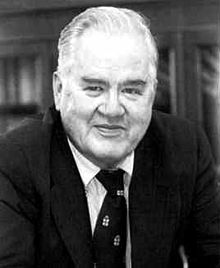
\includegraphics[width=\textwidth]{John_Tukey}
%%     \end{column}
%%     \begin{column}{0.6\textwidth}
%%       \begin{itemize}
%%       \item American statistician, 1915--2000
%%       \item Big fan of exploratory data analysis
%%       \item Invented boxplot
%%       \item Invented ``honestly significant differences''
%%       \item Invented jackknife estimation
%%       \item Coined computing term ``bit''
%%       \item Co-inventor of Fast Fourier Transform
%%       \end{itemize}
%%     \end{column}
%%   \end{columns}
%%   
%% \end{frame}
%% 
%% \begin{frame}[fragile]{Honestly Significant Differences}
%% 
%%   \begin{itemize}
%%   \item Compare several groups with \emph{one} test, telling you which
%%     groups differ from which.
%%   \item Idea: if all population means equal, find distribution of
%%     highest sample mean minus lowest sample mean.
%%   \item Any means unusually different compared to that declared
%%     significantly different.
%% 
%%   \end{itemize}
%%   
%% \end{frame}
%% 
%% \begin{frame}[fragile]{Tukey on rat data}
%% 
%% <<echo=F>>=
%% options(width=60)
%% @   
%% <<>>=
%% rats.aov=aov(density~group,data=rats)
%% TukeyHSD(rats.aov)
%% @   
%% 
%% Again conclude that bone density for \texttt{highjump} group significantly
%%   higher than for other two groups.
%%   
%% \end{frame}
%% 
%% 
%% 
%% \begin{frame}[fragile]{Why Tukey's procedure better than all
%%     $t$-tests}
%% 
%% Look at P-values for the two tests:
%% 
%% \begin{verbatim}
%% Comparison        Tukey    t-tests
%% ----------------------------------
%% Highjump-Control 0.0016     0.0021
%% Lowjump-Control  0.4744     0.2977
%% Lowjump-Highjump 0.0298     0.0045
%% \end{verbatim}
%% 
%% \begin{itemize}
%% \item Tukey P-values (mostly) higher.
%% \item Proper adjustment for doing \emph{three} $t$-tests at once, not
%%   just one in isolation.
%% \item \texttt{lowjump-highjump} comparison no longer significant at
%%   $\alpha=0.01$. 
%% \end{itemize}
%% 
%%   
%% \end{frame}

\begin{frame}[fragile]{Tukey in SAS}
  
  R equivalent: \texttt{TukeyHSD}.

\begin{Sascode}[store=ii]
proc anova;
  class group;
  model density=group;
  means group / tukey;
\end{Sascode}

Strategy: if you intend to do Tukey (if the ANOVA comes out
significant), submit \emph{all} these lines the first time. If the
ANOVA $F$-test is not significant, \emph{ignore} the Tukey.
   
\end{frame}

\begin{frame}[fragile]{Tukey output (some)}

\Listing[store=ii,objects=MCLines]{iii}
  
\end{frame}
%% 
%% \begin{frame}[fragile]{Checking assumptions}
%% 
%% <<fig.height=3>>=
%% ggplot(rats,aes(y=density,x=group))+geom_boxplot()
%% @   
%% 
%% 
%% 
%% Assumptions:
%% 
%% \begin{itemize}
%% \item Normally distributed data within each group
%% \item with equal group SDs.
%% \end{itemize}
%% 
%% 
%% \end{frame}
%% 
%% \begin{frame}[fragile]{The assumptions}
%% 
%%   \begin{itemize}
%%   \item Normally-distributed data within each group
%%   \item Equal group SDs.
%%   \end{itemize}
%% 
%% These are shaky here because:
%% 
%% \begin{itemize}
%% \item \texttt{control} group has outliers
%% \item \texttt{highjump} group appears to have less spread than others.
%% \end{itemize}
%% 
%% Possible remedies (in general):
%% 
%% \begin{itemize}
%% \item Transformation of response (usually works best when SD increases
%%   with mean)
%% \item If normality OK but equal spreads not, can use \textbf{Welch
%%     ANOVA}. (Regular ANOVA like pooled $t$-test; Welch ANOVA like
%%   Welch-Satterthwaite $t$-test.)
%% \item Can also use Mood's Median Test (see over). This works for any
%%   number of groups.
%% \end{itemize}
%% 
%% \end{frame}
%% 
%% \begin{frame}[fragile]{Mood's median test 1/3}
%%   
%%   \begin{itemize}
%%   \item Find median of \emph{all} bone densities, regardless of group:
%% <<>>=
%% m=median(rats$density) ; m
%% @     
%% \item Count up how many observations \emph{in each group} above or
%%   below overall median:
%%   
%%   \begin{multicols}{2}
%% <<>>=
%% tab=with(rats,
%%   table(group,density>m))
%% tab
%% @   
%% 
%% \item All \texttt{Highjump} obs above overall median.
%% \item Most \texttt{Control} obs \emph{below} overall median.
%% \item Suggests medians differ by group.
%%   \end{multicols}
%%   \end{itemize}
%%   
%% \end{frame}
%% 
%% \begin{frame}[fragile]{Mood's median test 2/3}
%%   
%%   \begin{itemize}
%%   \item Test whether association between group and being above/below
%%     overall median significant using \emph{chi-squared test for association}:
%%     
%% <<>>=
%% chisq.test(tab,correct=F)
%% @     
%% 
%% \item Very small P-value says that being above/below overall median
%%   \emph{depends on group}.
%% \item That is, groups \emph{do not} all have same median.
%%   
%%   \end{itemize}
%%   
%% \end{frame}
%% 
%% \begin{frame}[fragile]{Mood's median test 3/3}
%%   
%%   Or with \texttt{median\_test} from \texttt{smmr}, same as before:
%%   
%% <<>>=
%% median_test(rats,density,group)
%% @   
%% 
%% No doubt that medians differ by group.
%%   
%% \end{frame}
%% 
%% \begin{frame}[fragile]{Comments}
%%   
%%   \begin{itemize}
%%   \item This test is equivalent of $F$-test, not of Tukey.
%% \item To determine which groups differ from which, can compare all
%%   possible pairs of groups via (2-sample) Mood's median tests, then
%%   adjust P-values by multiplying by number of 2-sample Mood tests done.
%%   \end{itemize}
%%   
%% \end{frame}
%% 
%% \begin{frame}[fragile]{Welch ANOVA}
%%   
%%   \begin{itemize}
%%   \item For these data, Mood's median test probably best because we
%%     doubt both normality and equal spreads.
%%     \item When normality OK but \emph{spreads differ}, Welch ANOVA way
%%       to go. 
%%   \item Welch ANOVA done by \texttt{oneway.test} as shown (for illustration):
%%     
%% <<>>=
%% oneway.test(density~group,data=rats)
%% @     
%% \item P-value very similar, as expected.
%% \item Appropriate Tukey-equivalent here called Games-Howell (not done here).
%%   \end{itemize}
%%   
%% \end{frame}

\begin{frame}[fragile]{Mood's median test}
  
  \begin{Sascode}[store=ja]
proc npar1way median;
  var density;
  class group;
  \end{Sascode}
  
  Output part 1, confirming number of \texttt{density} values above
  grand median in each group:
  
\Listing[store=ja, fontsize=footnotesize, objects=medianScores]{jaa}
  
\end{frame}

\begin{frame}[fragile]{Rest of output}
  
\Listing[store=ja, fontsize=footnotesize, objects=medianAnalysis]{jab} 
  
Because there are more than 2 groups, we only get the chi-squared
test. This is (strongly) significant, so the median bone densities in
the three groups are not all the same.

\end{frame}

\begin{frame}[fragile]{Welch ANOVA in SAS}
  
R equivalent: \texttt{oneway.test}.  
  
The instruction to do the Welch ANOVA
goes on the \texttt{means} line, where the Tukey would go if we were
doing that:

\begin{Sascode}[store=jc]
proc anova;
  class group;
  model density=group;
  means group / hovtest=levene welch;
\end{Sascode}

Ignore the usual ANOVA in the output, and look right to the end:
  
\end{frame}

\begin{frame}[fragile]{Results}
  
  \Listing[store=jc, fontsize=footnotesize, objects=Welch Means]{jcc}

The Welch's ANOVA is the same as R's. Also note that the P-values for
the regular ANOVA (0.0019) and the Welch ANOVA (0.0023) are almost
identical here, so allowing for unequal spreads has made almost no
difference, even though the group SDs look different.
  
\end{frame}
%% games-howell
\begin{frame}[fragile]{Games-Howell}
  
  \begin{itemize}
  \item The approved multiple-comparisons test for Welch's ANOVA is
    Games-Howell, which can be done this way:
    
    \begin{Sascode}[store=rugap]
proc mixed;
  class group;
  model density=group / ddfm=satterth;
  repeated / group=group;
  lsmeans group / adjust=tukey adjdfe=row;
    \end{Sascode}
    
    
  \item In \texttt{group=group}, first \texttt{group} is always
    \texttt{group}, second one is name of your categorical
    variable. (Here that \emph{was} \texttt{group}.)
  \item There are (many other) details in the code, not explained here.
        
  \end{itemize}
  
\end{frame}

\begin{frame}[fragile]{Results}
  
    \Listing[store=rugap, fontsize=footnotesize, objects=diffs]{rugapp}
  
    High jumping significantly different from others (again).
  
\end{frame}
%% 
%\begin{frame}[fragile]{Randomization test}
%
%  \begin{itemize}
%  \item Like two-sample randomization test: randomly shuffle group memberships.
%  \item Choices about test statistic, eg.\
%    \begin{itemize}
%    \item usual ANOVA $F$-statistic
%    \item Tukey-like highest sample mean minus lowest
%    \end{itemize}
%  \item I go with highest minus lowest.
%
%
%  \end{itemize}
%\end{frame}
%
%\begin{frame}[fragile]{Observed means and test statistic}
%  
%  \begin{itemize}
%  \item Calculate observed value of test statistic:
%
%<<>>=
%group.means=aggregate(density~group,data=rats,mean) 
%group.means
%@     
%Actual means in second column of \texttt{group.means}:
%<<>>=
%z=group.means[,2]
%obs=max(z)-min(z)  
%obs
%@ 
%  \end{itemize}
%  
%\end{frame}
%
%\begin{frame}[fragile]{Randomly shuffling groups}
%
%Actual groups are:
%
%{\small
%<<>>=
%rats$group
%@ 
%}
%
%%$ %$
%
%Shuffle like this:
%
%<<echo=F>>=
%set.seed(457299)
%@ 
%
%{\small
%<<>>=
%shuffled.groups=sample(rats$group) ; shuffled.groups
%@   
%}
%
%\end{frame}
%
%\begin{frame}[fragile]{Calculate means and highest minus lowest}
%
%Same idea as for actual data, but using \texttt{shuffled.groups}
%instead of \texttt{group}:
%
%<<>>=
%my.group.means=aggregate(density~shuffled.groups,
%  data=rats,mean)
%my.group.means
%z=my.group.means[,2]
%max(z)-min(z)
%@ 
%
%Need to do this a bunch of times. Idea: write a function to do it
%once, then run function many times.
%
%
%\end{frame}
%
%\begin{frame}[fragile]{Function to do it once}
%  
%  \begin{itemize}
%  \item Input: original data.
%  \item Obtain shuffled groups
%  \item Calculate mean for each group
%  \item Return largest mean minus smallest mean.
%    
%  \item Function:
%  \end{itemize}
%  
%<<>>=
%shuffle1=function(mydata=rats) {
%  shuffled.groups=sample(mydata$group)
%  means=aggregate(density~shuffled.groups,
%    data=mydata,mean)
%  z=means[,2]
%  max(z)-min(z)
%}
%@   
%  
%\end{frame}
%
%
%
%\begin{frame}[fragile]{Obtaining randomization distribution}
%
%  \begin{itemize}
%  \item Test (randomizes, so look for ``sane'' answer):
%    
%<<>>=
%shuffle1(rats)
%@     
%
%\item Use \texttt{replicate} to do a few times:
%  
%<<>>=
%replicate(6,shuffle1(rats))
%@   
%
%\item Or many times, like 1000:
%  
%<<cache=T>>=
%test.stat=replicate(1000,shuffle1(rats))
%@   
%
%  \end{itemize}
%  
%\end{frame}
%
%
%\begin{frame}[fragile]{Randomization distribution of
%    \texttt{test.stat}}
%
%<<fig.height=3.7>>=
%vals=data.frame(ts=test.stat)
%ggplot(vals,aes(x=ts))+geom_histogram(binwidth=5)+
%  geom_vline(xintercept=obs,colour="red")
%#hist(test.stat)  
%#abline(v=obs,col="red")
%@   
%
%\end{frame}
%
%\begin{frame}[fragile]{Comments and P-value}
%
%  \begin{itemize}
%  \item Distribution shape skewed to right (lower limit of 0).
%  \item Red line marks observed highest minus lowest: seems unusually high.
%  \item If group means really different (anyhow), highest minus lowest
%    will be \emph{large}, so one-tailed test.
%  \item (Same logic as one-sidedness of $F$-test in ANOVA.)
%  \item P-value the usual way:
%    
%<<>>=
%table(test.stat>=obs)  
%@     
%\item P-value $2/1000=0.0020$. Despite outliers, still reject ``all
%  means equal'', with P-value very similar to ANOVA (0.0019).
%  \end{itemize}
%\end{frame}
%




 
% tidying and organizing data

\section{Tidying and organizing data}

\frame{\sectionpage}

  

%% \begin{frame}[fragile]{Reading in data}
%% 
%% <<echo=F, message=F>>=
%% require(tidyverse)
%% @   
%%   
%% <<size="small">>=
%% pigs1=read_delim("pigs1.txt"," ")
%% glimpse(pigs1)
%% @   
%%   
%% \end{frame}
%% 
%% \begin{frame}[fragile]{Gathering up the columns}
%%   
%%   \begin{itemize}
%%   \item This is a very common reorganization, and the magic ``verb''
%%     is \texttt{gather}:
%%     
%% <<>>=
%% pigs2=pigs1 %>% gather(feed,weight,feed1:feed4)
%% glimpse(pigs2)
%% @     
%% \item \texttt{pigs2} is now in ``long'' format, ready for analysis.
%% \item Anatomy of \texttt{gather}: what makes the columns different
%%   (different feeds), what makes them the same (all weights), which
%%   columns to combine.
%% \item Column \texttt{pig} now is 1--5 4 times (number of pig within
%%   each feed group). 
%%   \end{itemize}
%%   
%% \end{frame}
%% 
%% \begin{frame}[fragile]{\ldots and finally, the analysis}
%%   
%%   \begin{itemize}
%%   \item which is just what we saw before:
%%     
%% <<size="footnotesize">>=
%% weight.1=aov(weight~feed,data=pigs2)
%% summary(weight.1)
%% @     
%% \item The mean weights of pigs on the different feeds are definitely
%%   not all equal.
%%   
%% \item So we run Tukey to see which ones differ (over).
%%   \end{itemize}
%%   
%% \end{frame}
%% 
%% \begin{frame}[fragile]{Tukey}
%%   
%% <<size="small">>=
%% TukeyHSD(weight.1)
%% @   
%% 
%% All of the feeds differ! To find the best and worst, get mean weight
%% by feed group (over).
%%   
%% \end{frame}
%% 
%% \begin{frame}[fragile]{Mean weights by feed}
%%   
%%   I borrowed an idea from later to put the means in descending order:
%%   
%% <<>>=
%% pigs2 %>% group_by(feed) %>% 
%%   summarize(mean_weight=mean(weight)) %>%
%%   arrange(desc(mean_weight))
%% @   
%% 
%% Feed 3 is best, feed 1 worst.
%% \end{frame}
%% 
%% \begin{frame}[fragile]{Should we have any concerns about the ANOVA?}
%%   
%% <<fig.height=3.5>>=
%% ggplot(pigs2,aes(x=feed,y=weight))+geom_boxplot()
%% @   
%%   
%% Feed 2 has an outlier, but there are only 5 pigs in each group, and
%% the conclusion is so clear that I am OK with this.
%% \end{frame}
%% 
%% 
%% \begin{frame}[fragile]{Tuberculosis}
%%   
%%   \begin{itemize}
%%   \item The World Health Organization keeps track of number of cases
%%     of various diseases, eg.\ tuberculosis.
%%   \item Some data:
%% <<>>=
%%   tb=read_csv("tb.csv")
%% @ 
%% \item Variables (see over): country (abbreviated), year. Then number of cases
%%   for each gender and age group, eg.\ \texttt{m1524} is males aged
%%   15--24. Also \texttt{mu} and \texttt{fu}, where age is unknown.
%% \item Lots of missings. Want to get rid of.
%%   \end{itemize}
%%   
%% \end{frame}
%% 
%% \begin{frame}[fragile]{The data}
%% 
%% <<size="footnotesize">>=
%% tb
%% @   
%%   
%% \end{frame}
%% 
%% \begin{frame}[fragile]{Gather the gender-age group columns}
%% 
%% <<>>=
%%   tb2=tb %>% gather(genage,freq,m04:fu,na.rm=T)
%% @   
%% 
%% \begin{itemize}
%% \item what makes the columns-to-be-gathered different, then
%% \item what makes them the same, then
%% \item the columns to gather, then (optionally)
%% \item get rid of the missing values.
%% \end{itemize}
%% 
%% \end{frame}
%% 
%% \begin{frame}[fragile]{Results}
%%   
%% <<>>=
%% tb2
%% @   
%%   
%% \end{frame}
%% 
%% \begin{frame}[fragile]{Separating}
%%   
%%   \begin{itemize}
%%   \item 4 columns, but 5 variables, since \texttt{genage} contains
%%     both gender and age group. Split that up using \texttt{separate}.
%%   \item \texttt{separate} needs 3 things:
%%     \begin{itemize}
%%     \item what to separate (no quotes needed),
%%   \item what to separate into (here you \emph{do} need quotes),
%%   \item how to split.
%%     \end{itemize}
%%   \item For ``how to split'', here ``after first character'':
%% <<>>=
%%   tb3=tb2 %>% separate(genage,c("gender","age"),1)
%% @     
%%   \end{itemize}
%%   
%%   
%% \end{frame}
%% 
%% \begin{frame}[fragile]{Tidied tuberculosis data}
%%   
%% <<>>=
%% tb3
%% @   
%%   
%% \end{frame}
%% 
%% \begin{frame}[fragile]{In practice\ldots}
%%   
%%   \begin{itemize}
%%   \item instead of doing the pipe one step at a time, you \emph{debug}
%%     it one step at a time, and when you have each step working, you
%%     use that step's output as input to the next step, thus:
%% 
%% <<>>=
%%   tb3=tb %>% gather(genage,freq,m04:fu,na.rm=T) %>%
%%              separate(genage,c("gender","age"),1)
%% @     
%%     
%% \item You can split the R code over as many lines as you like,
%%   \emph{as long as each line is incomplete}, so that R knows more is
%%   to come.
%% \item I like to put the pipe symbol on the end of the line.
%%   \end{itemize}
%%   
%% \end{frame}
%% 
%% \begin{frame}[fragile]{Total tuberculosis cases by year}
%%   
%% <<>>=
%% s=tb3 %>% group_by(year) %>% summarize(cases=sum(freq))
%% @   
%% 
%% \begin{multicols}{3}
%% <<size="small">>=
%% s %>% slice(1:10)
%% @     
%% 
%% <<size="small">>=
%% s %>% slice(11:20)
%% @ 
%% 
%% <<size="small">>=
%% s %>% slice(21:29)
%% @ 
%%   
%%   \end{multicols}
%%   
%%   Something very interesting happened between 1994 and 1995.
%% \end{frame}
%% 
%% \begin{frame}[fragile]{Some weather data}
%% 
%% <<size="footnotesize">>=
%% weather=read_csv("weather.csv")
%% @     
%% 
%% \end{frame}
%% 
%% \begin{frame}[fragile]{The data}
%%   
%% <<size="footnotesize">>=
%% weather
%% @   
%%   
%% \end{frame}
%% 
%% \begin{frame}[fragile]{The columns}
%%   
%%   These are daily weather records for a weather station in Mexico.
%%   
%%   \begin{description}
%%   \item[\texttt{id}:] identifier for this weather station (always same here)
%%   \item[\texttt{year}, \texttt{month}:] obvious
%%   \item[\texttt{element}:] whether temperature given was daily max or
%%     daily min
%%   \item[\texttt{d1, d2,...}:] day of the month from 1st to 31st.
%%   \end{description}
%%   
%%   Numbers in data frame all temperatures (for different days of the
%%   month), so first step is
%% <<>>=
%% weather2= weather %>% gather(day,temperature,d1:d31,na.rm=T)    
%% @   
%%   
%% \end{frame}
%% 
%% \begin{frame}[fragile]{Results}
%% 
%% <<>>=
%% weather2
%% @   
%%   
%% \end{frame}
%% 
%% \begin{frame}[fragile]{The days}
%%   
%%   \begin{itemize}
%%     \item Column \texttt{element} contains \emph{names of two different
%%         variables}, that should each be in separate column.
%%     \item Distinct from eg.\ \texttt{m1524} in tuberculosis data, that
%%       contained \emph{levels of two different factors}, handled by \texttt{separate}.
%%     \item Untangling names of variables handled by \texttt{spread}:
%% <<>>=
%% weather3= weather %>% 
%%   gather(day,temperature,d1:d31,na.rm=T) %>%
%%   spread(element,temperature)
%% @ 
%%   \end{itemize}
%%   
%% \end{frame}
%% 
%% \begin{frame}[fragile]{Result}
%%   
%% <<>>=
%% weather3
%% @   
%%   
%% \end{frame}
%% 
%% \begin{frame}[fragile]{Further improvements}
%%   
%%   \begin{itemize}
%%   \item We have tidy data now, but can improve things further.
%%   \item \texttt{mutate} creates new columns from old (or assign back
%%     to change a variable).
%% 
%%   \item Would like the numerical dates. \texttt{separate} works, but
%%     also produces column named \texttt{d} whose value is always
%%     \texttt{d}. Instead pull out number as below.
%% 
%%   \item \texttt{select} keeps columns (or drops, with minus). Station
%%   \texttt{id} has no value to us:
%% 
%% <<>>=
%% weather4= weather %>% 
%%   gather(day,temperature,d1:d31,na.rm=T) %>%
%%   spread(element,temperature) %>%
%%   mutate(day=parse_number(day)) %>%
%%   select(-id)    
%% @     
%% 
%%   \end{itemize}
%%   
%% \end{frame}
%% 
%% \begin{frame}[fragile]{Results}
%%   
%% <<>>=
%% weather4
%% @   
%% \end{frame}
%%   
%% \begin{frame}[fragile]{Final step(s)}
%% 
%%   \begin{itemize}
%%   \item Make year-month-day into proper date.
%%   \item Keep only \texttt{date, tmax, tmin}:
%% 
%% <<>>=
%% weather5= weather %>% 
%%   gather(day,temperature,d1:d31,na.rm=T) %>%
%%   spread(element,temperature) %>%
%%   mutate(day=parse_number(day)) %>%
%%   select(-id) %>% 
%%   unite(datestr,c(year,month,day),sep="-") %>%
%%   mutate(date=as.Date(datestr)) %>%
%%   select(c(date,tmax,tmin))  
%% @ 
%%   \end{itemize}
%% 
%%     
%% \end{frame}
%% 
%% \begin{frame}[fragile]{Final results}
%% 
%% <<>>=
%% weather5
%% @   
%%   
%% \end{frame}
%% 
%% \begin{frame}[fragile]{Plotting the temperatures}
%%   
%%   \begin{itemize}
%%   \item Plot temperature against date joined by lines, but with
%%     separate lines for max and min.
%%   \item \texttt{ggplot} requires something like
%% <<eval=F>>=
%% ggplot(weather5,aes(x=date,y=temperature))
%% @     
%% only we have \emph{two} temperatures, one a max and one a min, that we
%% want to keep separate.
%% \item The trick: combine \texttt{tmax}  and \texttt{tmin} together
%%   into \emph{one} column, keeping track of what kind of temp they
%%   are. (This actually same format as \texttt{weather2}, which we said
%%   was ``untidy''.) Are making \texttt{weather5} untidy \emph{for
%%     purposes of drawing graph} only.
%% \item Then can do something like
%% <<eval=F>>=
%% ggplot(...,aes(x=date,y=temperature,colour=maxmin)
%% @   
%% to distinguish max and min on graph.
%%   \end{itemize}
%%   
%% \end{frame}
%% 
%% \begin{frame}[fragile]{Setting up plot}
%%   
%%   \begin{itemize}
%% \item Since we only need data frame for plot, we can do the
%%   column-creation and plot in a chain.
%% \item The temperature columns are actually text (see printout of
%%   \texttt{weather5}), but for graph they need to be numbers.
%%   \item For a \texttt{ggplot} in a chain, the initial data frame is
%%   omitted, because it is \emph{whatever came out of the previous step}.
%%   \item To make those ``one column''s: \texttt{gather} (result like \texttt{weather2}):
%%     
%% <<>>=
%% g=weather5 %>% 
%%   gather(maxmin,temperature,tmax:tmin) %>%
%%   mutate(temperature=as.numeric(temperature)) %>%
%%   ggplot(aes(x=date,y=temperature,colour=maxmin))+
%%     geom_line()
%% @     
%%   \end{itemize}
%%   
%% \end{frame}
%% 
%% \begin{frame}[fragile]{The plot}
%% 
%%   
%% <<fig.height=3.5>>=
%% g
%% @   
%%  
%% \end{frame}
%% 
%% %\begin{frame}[fragile]{The (computing) pipe}
%% %  
%% %  \begin{itemize}
%% %  \item Unix (and Linux) are built on small tools that do one thing
%% %    well.
%% %    
%% %  \item \texttt{grep} lists the lines of a file that match something:
%% %\begin{verbatim}
%% %bash> grep "dog" dog.txt
%% %My neighbour has a dog
%% %I like dogs.
%% %\end{verbatim}
%% %  \item You can also feed the output of one command into another:
%% %\begin{verbatim}
%% %bash> grep "dog" dog.txt | grep "neighbour"
%% %My neighbour has a dog
%% %\end{verbatim}
%% %  \item This obtains all the lines in the file that contain both
%% %    \texttt{dog} and \texttt{neighbour}. First finds all \texttt{dog} lines,
%% %    then ``pipes'' output of that into another \texttt{grep} that
%% %    finds all \texttt{neighbour} lines of result.
%% %  \item Pipe allows you to combine simple tools together.
%% %  \end{itemize}
%% %  
%% %\end{frame}
%% %
%% %\begin{frame}[fragile]{Pipes in \texttt{dplyr}}
%% %  
%% %  \begin{itemize}
%% %  \item In \texttt{weather}, got up to \texttt{weather8}, but really
%% %    only needed last one: many temporary variables, needed only to
%% %    hold output of one part until used as input to next (and then can
%% %    be thrown away).
%% %  \item \texttt{dplyr} has ``pipe'' mechanism, notated \texttt{\%>\%}.
%% %  \item Put on \emph{end} of line so that R knows more to come.
%% %  \end{itemize}
%% %  
%% %\end{frame}
%% %
%% %\begin{frame}[fragile]{Tuberculosis code (review)}
%% %  
%% %<<eval=F,cache=T>>=
%% %  tb=read.csv("tb.csv",header=T)
%% %  tb2=gather(tb,genage,freq,m04:fu,na.rm=T)
%% %  tb3=separate(tb2,genage,c("gender","age"),1)
%% %  aggregate(freq~year,tb3,sum)      
%% %@   
%% %
%% %Corresponding code using pipe is shorter:
%% %
%% %<<cache=T>>=
%% %  read.csv("tb.csv",header=T) %>%
%% %    gather(genage,freq,m04:fu,na.rm=T) %>%
%% %    separate(genage,c("gender","age"),1) %>%
%% %    aggregate(freq~year,.,sum) %>% head(4)
%% %@ 
%% %  
%% %\end{frame}
%% %
%% %\begin{frame}[fragile]{Comments}
%% %  
%% %  \begin{itemize}
%% %  \item Output from \texttt{read.csv} is data frame,
%% %    so its output fed straight into \texttt{gather}.
%% %  \item All the temporary variables have gone.
%% %  \item \texttt{gather}, \texttt{separate}, \texttt{head} shorter, and
%% %    \texttt{aggregate} different:
%% %    \begin{itemize}
%% %    \item If a function accepts data frame first, then the data frame
%% %      disappears in a pipe: ``whatever came out of the previous step''.
%% %    \item If function accepts data frame elsewhere, ``output from
%% %      previous stage of pipe'' replaced by a dot. 
%% %    \end{itemize}
%% %  \item To read: put word ``take'' before initial data frame and words
%% %    ``and then'' every time you see a pipe.
%% %  \item To save output from pipe in variable \texttt{x}, put
%% %    \texttt{x=} as usual at start of line. Alternatively, put
%% %    \texttt{-> x} at \emph{end}.
%% %  \end{itemize}
%% %  
%% %\end{frame}
%% %
%% %\begin{frame}[fragile]{Weather code as a (long) pipe}
%% %
%% %<<>>=
%% %read.csv("weather.csv",header=T) %>%
%% %   gather(day,temperature,d1:d31,na.rm=T) %>%
%% %   spread(element,temperature) %>%
%% %   mutate(day=extract_numeric(day)) %>%
%% %   select(-id) %>%
%% %   mutate(datestr=paste(year,month,day,sep="-")) %>%
%% %   mutate(date=as.Date(datestr)) %>%
%% %   select(c(date,tmax,tmin)) -> my_weather    
%% %@   
%% %
%% %
%% %\end{frame}
%% %
%% %\begin{frame}[fragile]{Results (some)}
%% %
%% %<<>>=
%% %tbl_df(my_weather)
%% %@   
%% %  
%% %\end{frame}
%% 
%% 
%% \begin{frame}[fragile]{Summary of tidying ``verbs''}
%%   
%%   \begin{tabular}{lp{0.7\textwidth}}
%%     Verb & Purpose\\
%%     \hline
%%     \texttt{gather}& Combine columns that measure same thing into one\\
%%     \texttt{spread}& Take column that measures one thing under
%%                      different conditions and put into multiple columns\\
%%     \texttt{separate} & Turn a column that encodes
%%                         several variables into
%%                         several columns\\
%%     \texttt{unite} & Combine several (related) variables into one
%%                      ``combination'' variable\\
%%     \hline
%%   \end{tabular}
%%   
%%   \texttt{gather} and \texttt{spread} are opposites; \texttt{separate}
%%   and \texttt{unite} are opposites.
%% \end{frame}
%% 
%% \begin{frame}[fragile]{Doing things with data frames}
%%   
%%   Let's go back to our Australian athletes:
%%   
%% <<echo=F,message=F>>=
%% athletes=read_tsv("ais.txt")
%% options(width=65)
%% @  
%% 
%% <<size="footnotesize">>=
%% athletes
%% @   
%% 
%% Following are some tasks that we might want to perform on this data frame.
%% \end{frame}
%% 
%% \begin{frame}[fragile]{Choosing a column}
%%   
%% <<>>=
%% athletes %>% select(Sport)
%% @   
%%   
%% \end{frame}
%% 
%% \begin{frame}[fragile]{Choosing several columns}
%%   
%% <<>>=
%% athletes %>% select(Sport,Hg,BMI)
%% @   
%%   
%% \end{frame}
%% 
%% \begin{frame}[fragile]{Choosing consecutive columns}
%%   
%% <<>>=
%% athletes %>% select(Sex:WCC)
%% @   
%%   
%% \end{frame}
%% 
%% \begin{frame}[fragile]{Choosing all-but some columns}
%%   
%% <<>>=
%% athletes %>% select(-(RCC:LBM))
%% @   
%%   
%% \end{frame}
%% 
%% \begin{frame}[fragile]{Select-helpers}
%%   
%%   Other ways to \texttt{select} columns:
%%   
%%   \begin{itemize}
%%   \item \texttt{starts\_with} something
%%   \item \texttt{ends\_with} something
%%   \item \texttt{contains} something
%%   \item \texttt{matches} a ``regular expression''
%%   \item \texttt{num\_range} like \texttt{x1} to \texttt{x3}
%%   \end{itemize}
%%   
%% \end{frame}
%% 
%% \begin{frame}[fragile]{Columns beginning with S}
%%   
%% <<>>=
%% athletes %>% select(starts_with("S"))
%% @   
%%   
%% \end{frame}
%% 
%% \begin{frame}[fragile]{Columns ending with C}
%%   
%%   either uppercase or lowercase:
%%   
%% <<>>=
%% athletes %>% select(ends_with("c"))
%% @   
%%   
%% \end{frame}
%% 
%% \begin{frame}[fragile]{Column names containing letter R}
%%   
%% <<>>=
%% athletes %>% select(contains("r"))
%% @   
%%   
%% \end{frame}
%% 
%% \begin{frame}[fragile]{Exactly two characters, ending with T}
%%   
%%   In regular expression terms, this is \verb=^.t$=: 
%%   %$ %$ %$
%%   \begin{itemize}
%%   \item   \verb=^= means ``start of text''
%%   \item \verb=.= means ``exactly one character, but could be
%%     anything''
%%     
%%   \item \verb=$= %$ %$ %$
%%     means ``end of text''.
%%   \end{itemize}
%%   
%% <<>>=
%% athletes %>% select(matches("^.t$"))
%% @   
%% %$ %$ %$
%% 
%% \end{frame}
%% 
%% \begin{frame}[fragile]{Displaying some numbered columns 1/2}
%%   
%% Make up a data frame to illustrate. This \texttt{sample} generates random
%% values equally likely to be anything 0--9 (without replacement):
%% 
%% <<>>=
%% d=tibble( y=sample(0:9,5),
%%           x1=sample(0:9,5),
%% 	  x2=sample(0:9,5),
%% 	  x3=sample(0:9,5))
%% d	  
%% @ 
%%   
%% \end{frame}
%% 
%% \begin{frame}[fragile]{Displaying some numbered columns 2/2}
%%   
%% Just display \texttt{x2} and \texttt{x3}:
%% 
%% <<>>=
%% d %>% select(num_range("x",2:3))
%% @ 
%%   
%% \end{frame}
%% 
%% \begin{frame}[fragile]{Displaying more than 10 rows}
%%   
%% <<size="footnotesize">>=
%% athletes %>% print(n=12)
%% @   
%%   
%% \end{frame}
%% 
%% \begin{frame}[fragile]{Displaying all the columns}
%%   
%% Just for 5 rows here:
%% 
%% <<size="footnotesize">>=
%% athletes %>% print(n=5, width=Inf)
%% @ 
%%   
%% \end{frame}
%% 
%% \begin{frame}[fragile]{Choosing rows by number}
%%   
%% <<>>=
%% athletes %>% slice(16:25)
%% @   
%%   
%% \end{frame}
%% 
%% \begin{frame}[fragile]{Non-consecutive rows}
%%   
%% <<>>=
%% athletes %>% slice(c(10,13,17,42))
%% @   
%%   
%% \end{frame}
%% 
%% \begin{frame}[fragile]{A random sample of rows}
%%   
%% <<>>=
%% athletes %>% sample_n(8)
%% @   
%%   
%% \end{frame}
%% 
%% \begin{frame}[fragile]{Rows for which something is true}
%%   
%% <<size="small">>=
%% athletes %>% filter(Sport=="Tennis")
%% @   
%%   
%% \end{frame}
%% 
%% \begin{frame}[fragile]{More complicated selections}
%%   
%% <<>>=
%% athletes %>% filter(Sport=="Tennis",RCC<5)
%% @   
%%   
%% \end{frame}
%% 
%% \begin{frame}[fragile]{Either/Or}
%%   
%% <<>>=
%% athletes %>% filter(Sport=="Tennis" | RCC>5) 
%% @   
%%   
%% \end{frame}
%% 
%% \begin{frame}[fragile]{Sorting into order}
%%   
%% <<>>=
%% athletes %>% arrange(RCC) 
%% @   
%%   
%% \end{frame}
%% 
%% \begin{frame}[fragile]{Breaking ties by another variable}
%%   
%% <<>>=
%% athletes %>% arrange(RCC,BMI)
%% @   
%%   
%% \end{frame}
%% 
%% \begin{frame}[fragile]{Descending order}
%%   
%% <<>>=
%% athletes %>% arrange(desc(BMI))
%% @   
%%   
%% \end{frame}
%% 
%% \begin{frame}[fragile]{``The top ones''}
%%   
%% <<>>=
%% athletes %>% arrange(desc(Wt)) %>% slice(1:7) %>% 
%%   select(Sport,Wt)
%% @   
%%   
%% \end{frame}
%% 
%% \begin{frame}[fragile]{Create new variables from old ones}
%%   
%% <<>>=
%% athletes %>% mutate(wt_lb=Wt*2.2) %>%
%%   select(Sport,Wt,wt_lb)
%% @   
%%   
%% \end{frame}
%% 
%% \begin{frame}[fragile]{Turning the result into a number}
%%   
%% Output is always data frame unless you explicitly turn it into
%% something else, eg.\ the weight of the heaviest athlete, as a number:
%% 
%% <<>>=
%% athletes %>% arrange(desc(Wt)) %>% slice(1) %>%
%%   pull(Wt)
%% @ 
%% 
%% All of these tools can be combined, as with this example.
%%   
%% \end{frame}
%% 
%% \begin{frame}[fragile]{To find the mean height of the women athletes}
%%   
%% Two ways:
%% 
%% <<>>=
%% athletes %>% group_by(Sex) %>% summarize(m=mean(Ht))
%% @ 
%% 
%% or
%% 
%% <<>>=
%% athletes %>% filter(Sex=="female") %>% summarize(m=mean(Ht))
%% @ 
%%   
%% \end{frame}
%% 
%% \begin{frame}[fragile]{Summary of data selection/arrangement ``verbs''}
%%   
%%   \begin{tabular}{lp{0.7\textwidth}}
%%     Verb & Purpose\\
%%     \hline
%%     \texttt{select} & Choose columns\\
%%     \texttt{print} & Display non-default \# of rows/columns \\
%%     \texttt{slice} & Choose rows by number\\
%%     \texttt{sample\_n} & Choose random rows\\ 
%%     \texttt{filter} & Choose rows satisfying conditions \\
%%     \texttt{arrange}& Sort in order by column(s) \\
%%     \texttt{mutate} & Create new variables\\
%%     \texttt{as.numeric}     & Turn result from data frame into number\\
%%     \texttt{group\_by} & Create groups to summarize by\\
%%     \texttt{summarize} & Calculate summary statistics (by groups if defined)\\
%%     \hline
%%   \end{tabular}
%%   
%% \end{frame}
%% 
%% \begin{frame}[fragile]{Looking things up in another data frame}
%%   
%%   Recall the tuberculosis data set, tidied:
%%   
%% <<size="footnotesize">>=
%% tb3
%% @   
%% 
%% What are actual names of those countries in \texttt{iso2}?
%%   
%% \end{frame}
%% 
%% \begin{frame}[fragile]{Actual country names}
%%   
%%   Found actual country names to go with those abbreviations, in spreadsheet:
%%   
%% <<>>=
%% library(readxl)
%% country_names=read_excel("ISOCountryCodes081507.xlsx")
%% @   
%%   
%% \end{frame}
%% 
%% \begin{frame}[fragile]{The country names}
%%   
%% <<>>=
%% country_names
%% @   
%%   
%% \end{frame}
%% 
%% \begin{frame}[fragile]{Looking up country codes}
%%   
%%   Matching a variable in one data frame to one in another is called a
%%   \textbf{join} (database terminology):
%%   
%% <<size="small">>=
%% tb3 %>% left_join(country_names,by=c("iso2"="Code_UC"))
%% @   
%%   
%% \end{frame}
%% 
%% \begin{frame}[fragile]{Total cases by country}
%%   
%% <<>>=
%% tb3 %>% group_by(iso2) %>% summarize(cases=sum(freq)) %>%
%%   left_join(country_names,by=c("iso2"="Code_UC")) %>%
%%   select(Country,cases)
%% @   
%%   
%% \end{frame}

\begin{frame}[fragile]{Some tidying and organizing in SAS}
  
  \begin{itemize}
  \item SAS is less flexible than R's \texttt{tidyverse} tools, but
    some of the previous can be done (with effort).
  \item Basic idea: create a new dataset using \texttt{data} and
    \texttt{set}, and then provide additional code to say what to do
    to the previous dataset.
  \item Read Australian athletes data again:
    
    \begin{Datastep}
filename myurl url 
  "http://www.utsc.utoronto.ca/~butler/c32/ais.txt";
proc import 
  datafile=myurl
  dbms=dlm
  out=sports
  replace;
  delimiter='09'x;
  getnames=yes;

    \end{Datastep}
    
  \end{itemize}
  
\end{frame}

\begin{frame}[fragile]{Check the data}
  
  \begin{Sascode}[store=ta]
proc print data=sports(obs=10);    
  \end{Sascode}
  
  \Listing[store=ta,fontsize=tiny]{taa}
  
\end{frame}

\begin{frame}[fragile]{Choosing variables}
  
  \texttt{keep} to say which ones you want:

  \begin{Datastep}
data sports2;
  set sports;
  keep Sport Sex Ht Wt;
  \end{Datastep}
  
  \begin{Sascode}[store=tb]
proc print data=sports2(obs=8);
  \end{Sascode}
  
  \Listing[store=tb]{tbb}
  
\end{frame}


\begin{frame}[fragile]{Un-choosing variables}
  
  \texttt{drop} to say which ones you don't want. Note the double-dash
  to denote ``this through that'':

  \begin{Datastep}
data sports3;
  set sports;
  drop RCC--LBM;
  \end{Datastep}
  
  \begin{Sascode}[store=tc]
    proc print data=sports3(obs=8);
  \end{Sascode}

    \Listing[store=tc,fontsize=small]{tcc}

\end{frame}

\begin{frame}[fragile]{Comments}
  
  \begin{itemize}
  \item Normally don't worry about explicitly dropping variables you
    don't need; you just ignore them in your analysis.
  \item \texttt{keep} and \texttt{drop} mostly for final ``tidy'' version of
    datasets that you create.
  \item Can also feed \texttt{proc print} the columns to display, with
    \texttt{var}. 
  \item For example, might want to discard intermediate steps of a
    calculation. 
  \item \texttt{keep} and \texttt{drop} equivalent to R
    \texttt{select}.
  \end{itemize}
  
\end{frame}

\begin{frame}[fragile]{Calculating a new variable}
  
  Put the calculation in the \texttt{data} step, as we have seen
  before. R equivalent: \texttt{mutate}.
  
  \begin{Datastep}
data sports4;
  set sports;
  Wt_lb=Wt*2.2;
  keep Sport Wt Wt_lb;
  \end{Datastep}
  
  \begin{Sascode}[store=td]
proc print data=sports4(obs=7);    
  \end{Sascode}
  
  \Listing[store=td, fontsize=small]{tdd}
  
\end{frame}


\begin{frame}[fragile]{Choosing rows by row number}
  
  SAS has a special variable \texttt{\_N\_} that holds the row
  number. R equivalent: \texttt{slice}.
  
  \begin{Datastep}
data sports5;
  set sports;
  if _N_>=16 and _N_<=25;
\end{Datastep}

\begin{Sascode}[store=te, fontsize=small]
proc print;  
\end{Sascode}

\Listing[store=te,fontsize=footnotesize]{tee}
  
\end{frame}

\begin{frame}[fragile]{Choosing each of a number of rows}
  
  \begin{Datastep}
data sports6;
  set sports;
  if _N_ in (10, 13, 17, 42);
  \end{Datastep}
  
  \begin{Sascode}[store=tf]
proc print;    
  \end{Sascode}
  
  \Listing[store=tf,fontsize=footnotesize]{tff}
\end{frame}

\begin{frame}[fragile]{Choosing rows where a condition is true}
  
  \texttt{if} like R's \texttt{filter}, but note that SAS uses
  \emph{one} equals sign in testing for equality:
  
  \begin{Datastep}
data sports7;
  set sports;
  if Sport="Tennis";
  \end{Datastep}
  \begin{Sascode}[store=tg]
proc print;    
  \end{Sascode}
  
  \Listing[store=tg,fontsize=scriptsize]{tgg}
  
\end{frame}

\begin{frame}[fragile]{Multiple conditions 1/2}
  
  Join them with actual words \texttt{and}, \texttt{or}:
  
  \begin{Datastep}
data sports8;
  set sports;
  if Sport="Tennis" and RCC<5;
  \end{Datastep}
  
  \begin{Sascode}[store=th]
proc print;
  var Sex--RCC;
  \end{Sascode}
  
  \Listing[store=th]{thh}
  
\end{frame}

\begin{frame}[fragile]{Multiple conditions 2/2}
  
  \begin{Datastep}
data sports9;
  set sports;
  if Sport="Tennis" or RCC>5;
  \end{Datastep}
  
  \begin{Sascode}[store=ti]
proc print;
  var Sex--RCC BMI;
  \end{Sascode}
  
  \Listing[store=ti,fontsize=tiny]{tii}
\end{frame}

\begin{frame}[fragile]{Using data \texttt{where} a condition is true}
  
  \begin{itemize}
  \item Rather than creating a new data set containing the values that
    satisfy a condition, we can tell SAS which data to use right in a
    \texttt{proc}.
  \item As near as SAS gets to R pipeline.
  \item Key idea: put \texttt{where} and a logical condition as the
    \emph{first} line of the \texttt{proc}.
  \item For example, mean BMI of tennis players:
    \begin{Sascode}[store=zawis]
proc means;
  where sport="Tennis";
  var BMI;
    \end{Sascode}
  \end{itemize}
  
\end{frame}

\begin{frame}[fragile]{Mean and SD of BMI for tennis players}
  
\Listing[store=zawis, fontsize=footnotesize]{zawiss}  
  
\end{frame}

\begin{frame}[fragile]{Arranging values in order}
  
  This is \texttt{proc sort}, which produces an output data set that
  is the ``most recent'' one. R equiv: \texttt{arrange}.
  
  \begin{Sascode}[store=tj]
proc sort data=sports;
  by RCC;
  
proc print;  
  var Sex--RCC;
  \end{Sascode}
  
  \Listing[store=tj,fontsize=footnotesize]{tjj}
  
\end{frame}

\begin{frame}[fragile]{Using a second variable as tiebreaker}
  
  
  \begin{Sascode}[store=tk]
proc sort data=sports;
  by RCC BMI;
  
proc print;  
  var Sex--RCC BMI;
  \end{Sascode}
  
  \Listing[store=tk,fontsize=footnotesize]{tkk}
  
\end{frame}

\begin{frame}[fragile]{Descending order}
  
  
  \begin{Sascode}[store=tl]
proc sort data=sports;
  by descending BMI;
  
proc print;  
  var Sex--RCC BMI;
  \end{Sascode}
  
  \Listing[store=tl,fontsize=footnotesize]{tll}
  
\end{frame}

\begin{frame}[fragile]{Displaying the seven heaviest athletes}
  
  \begin{Sascode}[store=tm]
proc sort data=sports;
  by descending Wt;
  
data sports10;
  set sports;
  if _N_<=7;
  keep Sport Wt;
  
proc print;
  \end{Sascode}
  
  \Listing[store=tm,fontsize=footnotesize]{tmm}
  
\end{frame}

\begin{frame}[fragile]{Tidying data}
\begin{itemize}
\item Data rarely come to us as we want to use them.
\item Before we can do analysis, typically have organizing to do.
\item This is typical of ANOVA-type data, ``wide format'':
  
  \verbatiminput{/home/ken/teaching/c32/notes/2017/pigs1.txt}
\item 20 pigs are randomly allocated to one of four feeds. At the end
  of the study, the weight of each pig is recorded, and we want to
  know whether there are any differences in mean weights among the
  feeds.
\item Problem: want the weights all in \emph{one} column, with 2nd
  column labelling which feed each weight was from. Untidy!
\end{itemize}
\end{frame}

  \begin{frame}[fragile]{Tidy and untidy data (Wickham)}
  
  \begin{itemize}
  \item Data set easier to deal with if:
    \begin{itemize}
    \item each observation is one \emph{row}
    \item each variable is one \emph{column}
    \item each type of observation unit is one \emph{table}
    \end{itemize}

  \item Data arranged this way called ``tidy''; otherwise called
    ``untidy''.
  \item For the pig data, response variable is weight, but scattered
    over 4 columns, which are \emph{levels} of a factor \texttt{feed}.
  \item Want all the weights in \emph{one} column, with a second
    column \texttt{feed} saying which feed that weight goes with, like
    R \texttt{gather}.
  \item Then we can run \texttt{proc anova}.
    
    

    
  \end{itemize}

  

  
\end{frame}


\begin{frame}[fragile]{Tidying data in SAS}
  
  \begin{itemize}
  \item Hard. Illustrate the SAS version
    of \texttt{gather} on the pigs data, that we have to read in first.
  \item Each line of this dataset has to produce \emph{four} lines
    of the long data set. 
    
    \begin{Datastep}
filename myurl url 
  "http://www.utsc.utoronto.ca/~butler/c32/pigs1.txt";      
proc import 
  datafile=myurl
  dbms=dlm out=pigs replace;
  delimiter=' ';
  getnames=yes;
    \end{Datastep}
    
    \begin{Sascode}[store=tn]
proc print;      
    \end{Sascode}
    
    \Listing[store=tn,fontsize=scriptsize]{tnn}
    
  \end{itemize}
  
\end{frame}

\begin{frame}[fragile]{Making the long data set, the tedious way}
  
  \begin{Datastep}
data pigs2;
  set pigs;
  feed='feed1';
  weight=feed1;
  output;
  feed='feed2';
  weight=feed2;
  output;
  feed='feed3';
  weight=feed3;
  output;
  feed='feed4';
  weight=feed4;
  output;
  keep feed weight;
  \end{Datastep}
  
\end{frame}

\begin{frame}[fragile]{The long data set}
  
  \begin{Sascode}[store=to]
proc print;    
  \end{Sascode}
  
\Listing[store=to,fontsize=scriptsize]{too}  
  
\end{frame}

\begin{frame}[fragile]{Using a SAS array to reduce repetition}

  \begin{Datastep}
data pigs3;
  set pigs;
  array feed_array [4] feed1-feed4;
  do i=1 to 4;
    weight=feed_array[i];
    feed=vname(feed_array[i]);
    output;
  end;
  keep pig feed weight;
  \end{Datastep}
  
  \begin{itemize}
  \item   In SAS, an array is a mechanism for referring to a group of
  variables together, here the four feed variables. The $i$-th element
  of the array refers to the $i$-th feed variable.
\item In the loop (indented), \texttt{weight} is set to the
  \emph{value} of the appropriate one of the \texttt{feed} variables,
  while \texttt{feed} is set to the \emph{name} of that \texttt{feed}
  variable. Compare the coding without the loop.
  \end{itemize}
  
  
\end{frame}

\begin{frame}[fragile]{The long data set, again}
  
  \begin{Sascode}[store=tp]
proc print;    
  \end{Sascode}
  
\Listing[store=tp,fontsize=scriptsize]{tpp}  
  
\end{frame}

\begin{frame}[fragile]{The ANOVA, again, with output part 1}
  
  \begin{Sascode}[store=tr]
proc anova;
  class feed;
  model weight=feed;
  means feed / tukey;
  \end{Sascode}
  
\Listing[store=tr,fontsize=scriptsize,objects=overallanova modelanova]{trs} 

The mean weights are not all the same for each feed.

\end{frame}

\begin{frame}[fragile]{Tukey output}
  
\Listing[store=tr,fontsize=footnotesize,objects=mclines]{trr}  
  

All of the feeds have significantly different mean weight, with feed 3
being the best and feed 1 the worst.
\end{frame}

% case studies


%% \section{Case study 1: the windmill data}
%% 
%% \frame{\sectionpage}
%% 
%% % ex2.swv
%% 
%% \begin{frame}[fragile]{R packages used}
%%   
%% <<size="scriptsize">>=
%% library(tidyverse)
%% library(broom)
%% library(MASS)
%% library(leaps)
%% @   
%%   
%% \end{frame}

%% \begin{frame}[fragile]{The windmill data}
%% 
%%   \begin{itemize}
%%   \item Engineer: does amount of electricity generated by windmill
%%     depend on how strongly wind blowing?
%%   \item Measurements of wind speed and DC current generated at various times.
%%   \item Assume the ``various times'' to be randomly selected --- aim
%%     to generalize to ``this windmill at all times''.
%%   \item Research questions:
%%     \begin{itemize}
%%     \item Relationship between wind speed and current generated?
%%     \item If so, what kind of relationship?
%%     \item Can we model relationship to do predictions?
%%     \end{itemize}
%%   \item Do analysis in R.
%%   \end{itemize}
%% 
%% \end{frame}
%% 
%% \begin{frame}[fragile]{Reading in the data}
%% 
%% <<>>=
%% windmill=read_csv("windmill.csv")
%% @ 
%% 
%% \end{frame}
%% 
%% \begin{frame}[fragile]{The data}
%%   
%% <<>>=
%% windmill
%% @   
%%   
%% \end{frame}
%% 
%% 
%% \begin{frame}[fragile]{Strategy}
%% 
%%   \begin{itemize}
%%   \item Two quantitative variables, looking for relationship:
%%     regression methods.
%%   \item Start with picture (scatterplot).
%%   \item Fit models and do model checking, fixing up things as necessary.
%%   \item Scatterplot:
%%     \begin{itemize}
%%     \item 2 variables, \texttt{DC\_output} and \texttt{wind\_velocity}.
%%     \item First is output/response, other is input/explanatory.
%%     \item Put \texttt{DC\_output} on vertical scale.
%%     \item Add trend, but don't want to assume linear.
%% 
%% 
%% <<>>=
%% g=ggplot(windmill,aes(y=DC_output,x=wind_velocity))+
%%   geom_point()+geom_smooth(se=F)
%% @ 
%%     \end{itemize}
%%   
%% 
%%   \end{itemize}
%% 
%% 
%% \end{frame}
%% 
%% 
%% \begin{frame}[fragile]{Scatterplot}
%% 
%% <<fig.height=4>>=
%% g
%% @ 
%% 
%% 
%% \end{frame}
%% 
%% 
%% \begin{frame}[fragile]{Comments}
%% 
%%   \begin{itemize}
%%   \item Definitely a relationship: as wind velocity increases, so does
%%     DC output. (As you'd expect.)
%%   \item Is relationship linear? To help judge, \emph{geom\_smooth}
%%     smooths scatterplot trend. (Trend called ``loess'', ``Locally
%%     weighted least squares'' which downweights outliers. Not
%%     constrained to be straight.)
%%   \item Trend more or less linear for while, then curves
%%     downwards. Straight line not so good here.
%%   \end{itemize}
%% 
%% \end{frame}
%% 
%% \begin{frame}[fragile]{Fitting a straight line}
%% 
%%   \begin{itemize}
%%   \item Let's try fitting a straight line anyway, and see what
%%     happens:
%% {\footnotesize
%% <<>>=
%% DC.1=lm(DC_output~wind_velocity,data=windmill)
%% summary(DC.1)  
%% @   
%% }
%%   \end{itemize}
%%   
%% \end{frame}
%% 
%% 
%% 
%% \begin{frame}[fragile]{Comments}
%% 
%%   \begin{itemize}
%%   \item Strategy: \texttt{lm} actually fits the regression. Store
%%     results in a variable. \emph{Then} look at the results, eg.\ via
%%     \texttt{summary}. 
%%   \item My strategy for model names: use response variable and a
%%     number. Allows me to fit several models to same data and keep
%%     track of which is which.
%%   \item Results actually pretty good: \texttt{wind.velocity} strongly
%%   significant, R-squared (87\%) high.
%% \item How to check whether regression is appropriate? Look at the
%%   \emph{residuals}, observed minus predicted.
%%   \item Plot using the regression object as ``data frame'':
%% 
%% <<>>=
%% g=ggplot(DC.1,aes(y=.resid,x=.fitted))+
%%   geom_point()+geom_smooth(se=F)
%% @ 
%% 
%% 
%% 
%%   \end{itemize}
%% \end{frame}
%% 
%% \begin{frame}[fragile]{Plot of residuals against fitted values}
%% 
%% <<fig.height=4>>=
%% g
%% @ 
%%   
%% 
%% \end{frame}
%% 
%% \begin{frame}[fragile]{Comments on residual plot}
%% 
%%   \begin{itemize}
%%   \item Residual plot should be a random scatter of points.
%%   \item Should be no pattern ``left over'' after fitting the regression.
%%   \item Smooth trend should be more or less straight across
%%     at 0.
%%   \item Here, have a \emph{curved} trend on residual plot.
%%   \item This means original relationship must have been a curve (as we
%%     saw on original scatterplot).
%%   \item Possible ways to fit a curve:
%%     \begin{itemize}
%%     \item Add a squared term in explanatory variable.
%%     \item Transform response variable (doesn't work well here).
%%     \item See what science tells you about mathematical form of
%%       relationship, and try to apply.
%%     \end{itemize}
%%   \end{itemize}
%% \end{frame}
%% 
%% \begin{frame}[fragile]{Parabolas and fitting parabola model}
%% 
%%   \begin{itemize}
%%   \item A parabola has equation
%%     $$ y= ax^2+bx+c $$
%%     for suitable $a, b, c$. About the simplest function that is not a
%%     straight line.
%%   \item Fit one using \texttt{lm} by adding $x^2$ to right side of
%%     model formula with \texttt{+}: 
%% 
%% <<>>=
%% DC.2=lm(DC_output~wind_velocity+I(wind_velocity^2),
%%   data=windmill)
%% @       
%% 
%% \item The \texttt{I()} necessary because \verb+^+ in model formula
%%   otherwise means something different (to do with interactions in ANOVA).
%% 
%% \item This actually \emph{multiple regression}.
%% \item Call it \emph{parabola model}.
%% 
%% 
%%   \end{itemize}
%% 
%% \end{frame}
%% 
%% \begin{frame}[fragile]{Parabola model output}
%% 
%% {\footnotesize
%% <<>>=
%% summary(DC.2)  
%% @ 
%% }
%% 
%% \end{frame}
%% 
%% \begin{frame}[fragile]{Comments on output}
%% 
%%   \begin{itemize}
%%   \item R-squared has gone up a lot, from 87\% (line) to 97\% (parabola).
%%   \item Coefficient of squared term strongly significant (P-value
%%     $6.59 \times 10^{-8}$).
%%   \item Adding squared term has definitely improved fit of model.
%%   \item Parabola model \emph{better} than linear one.
%%   \item But\ldots need to check residuals again:
%% 
%% <<>>=
%% g=ggplot(DC.2,aes(y=.resid,x=.fitted))+
%%   geom_point()
%% @ 
%% 
%%   \end{itemize}
%% 
%% \end{frame}
%% 
%% \begin{frame}[fragile]{Residual plot from parabola model}
%% 
%% <<fig.height=4>>=
%% g
%% @ 
%% 
%% 
%% \end{frame}
%% 
%% \begin{frame}[fragile]{Or, with smooth trend}
%%   
%% <<fig.height=4>>=
%% g+geom_smooth(se=F)
%% @   
%%   
%% \end{frame}
%% 
%% \begin{frame}[fragile]{Scatterplot with fitted line and curve}
%% 
%%   \begin{itemize}
%% 
%% \item Residual plot basically random. Good.
%% \item Smooth trend \emph{not} flat, but might be deceived by few
%%   residuals above 0 in middle.
%%   \item Scatterplot with fitted line and curve like this:
%% 
%% <<>>=
%% g=ggplot(windmill,aes(y=DC_output,x=wind_velocity))+
%%   geom_point()+geom_smooth(method="lm",se=F)+
%%   geom_line(data=DC.2,aes(y=.fitted))
%% @     
%% 
%%   \item This plots: scatterplot (\verb-geom_point-);
%%   straight line (via tweak to \verb-geom_smooth-, which
%%     draws best-fitting line);
%%   fitted curve, using the predicted \texttt{DC\_output}
%%     values, joined by lines (with points not shown).
%%   \item Trick in the \verb-geom_line- is use the \emph{predictions} as
%%     the $y$-points to join by lines (from \texttt{DC.2}), instead of
%%     the original data points. Without the \texttt{data} and
%%     \texttt{aes} in the \verb-geom_line-, \emph{original data points}
%%     would be joined by lines.
%% 
%% \end{itemize}
%%   
%% \end{frame}
%% 
%% 
%% \begin{frame}[fragile]{Scatterplot with fitted line and curve}
%% 
%% <<fig.height=3.7>>=
%% g
%% @     
%%   
%% Curve clearly fits better than line.
%% 
%% 
%% \end{frame}
%% 
%% \begin{frame}[fragile]{Another approach to a curve}
%% 
%%   \begin{itemize}
%%   \item There is a problem with parabolas, which  we'll see later.
%%   \item Go back to engineer with findings so far. Ask, ``what should
%%     happen as wind velocity increases?'':
%%     \begin{quote}
%%       Upper limit on electricity generated, but otherwise, the larger the
%%       wind velocity, the more electricity generated.
%%     \end{quote}
%%   \item Mathematically, sounds like \emph{asymptote}. Straight lines
%%     and parabolas don't have them, but eg.\ $y=1/x$ does: as $x$ gets
%%     bigger, $y$ approaches zero without reaching it.
%%   \item What happens to $y=a+b(1/x)$ as $x$ gets large?
%%   \item $y$ gets closer and closer to $a$ --- $a$ is asymptote.
%%   \item Fit this, call it \emph{asymptote model}.
%%   \item Fitting the model here \emph{because we have math to justify
%%       it}. 
%%   \item Alternative, $y=a+be^{-x}$, approaches asymptote faster.
%%   \end{itemize}
%% 
%% \end{frame}
%% 
%% 
%% 
%% \begin{frame}[fragile]{How to fit asymptote model?}
%% 
%%   \begin{itemize}
%%   \item Same idea as for parabola: define new explanatory variable to
%%     be $1/x$, and predict $y$ from it.
%%   \item $x$ is velocity, distance over time.
%%   \item So $1/x$ is time over distance. In walking world, if you walk
%%     5 km/h, take 12 minutes to walk 1 km, called your \emph{pace}. So call
%%     1 over \texttt{wind\_velocity} \texttt{wind\_pace}.
%%   \item Make a scatterplot first to check for straightness (next page)
%% 
%% <<>>=
%% windmill$wind_pace=1/windmill$wind_velocity
%% g=ggplot(windmill,aes(y=DC_output,x=wind_pace))+
%%   geom_point()+geom_smooth(se=F)
%% @     
%% 
%% \item and run regression like this (page after):
%% <<>>=
%% DC.3=lm(DC_output~wind_pace,data=windmill)
%% @ 
%% 
%% 
%%   \end{itemize}
%% 
%% \end{frame}
%% 
%% \begin{frame}[fragile]{Scatterplot for \texttt{wind\_pace}}
%% 
%% <<fig.height=3.7>>=
%% g
%% @     
%% 
%%       That's pretty straight.
%% 
%% 
%% 
%% \end{frame}
%% 
%% \begin{frame}[fragile]{Regression output}
%% 
%%   {\footnotesize
%% <<echo=F>>=
%% summary(DC.3)  
%% @ 
%% }
%% 
%% \end{frame}
%% 
%% \begin{frame}[fragile]{Comments}
%% 
%%   \begin{itemize}
%%   \item R-squared, 98\%, even higher than for parabola model (97\%).
%%   \item Simpler model, only one explanatory variable
%%     (\texttt{wind.pace}) vs.\ 2 for parabola model
%%     (\texttt{wind.velocity} and its squareXS).
%%   \item \texttt{wind.pace} (unsurprisingly) strongly significant.
%%   \item Looks good, but check residual plot:
%% 
%% 
%% <<>>=
%% g=ggplot(DC.3,aes(y=.resid,x=.fitted))+
%%   geom_point()+geom_smooth(se=F)
%% @ 
%% 
%%   \end{itemize}
%% 
%% \end{frame}
%% 
%% 
%% 
%% \begin{frame}[fragile]{Residual plot for asymptote model}
%% 
%% <<fig.height=4>>=
%% g
%% @ 
%% 
%% \end{frame}
%% 
%% 
%% \begin{frame}[fragile]{Plotting trends on scatterplot}
%% 
%%   \begin{itemize}
%%   \item Residual plot not bad. But residuals go up to 0.10 and down to $-0.20$,
%%       suggesting possible skewness (not normal). I think it's not
%%       perfect, but OK overall.
%%     \item Next: plot scatterplot with \emph{all three} fitted
%%       lines/curves on it (for comparison), with legend saying which is
%%       which.
%%     \item First make data frame containing what we need, taken from
%%       the right places:
%%       
%% <<>>=
%% w2=tibble(wind_velocity=windmill$wind_velocity,
%%           DC_output=windmill$DC_output,
%% 	  linear=fitted(DC.1),
%% 	  parabola=fitted(DC.2),
%% 	  asymptote=fitted(DC.3))
%% @ 
%% 
%% 
%% 
%%   \end{itemize}
%% 
%% 
%%   
%% \end{frame}
%% 
%% \begin{frame}[fragile]{What's in ``w2''}
%%   
%% <<>>=
%% w2
%% @       
%%   
%% \end{frame}
%% 
%% \begin{frame}[fragile]{Making the plot}
%%   
%%   \begin{itemize}
%%   \item \texttt{ggplot} likes to have \emph{one} column of $x$'s to
%%     plot, and one column of $y$'s, with another column for
%%     distinguishing things.
%%   \item But we have \emph{three} columns of fitted values, that need
%%     to be combined into one.
%%   \item \texttt{gather}, then plot:
%%     
%% <<>>=
%% g=w2 %>% gather(model,fit,linear:asymptote) %>%
%%       ggplot(aes(x=wind_velocity,y=DC_output))+
%%       geom_point()+
%%       geom_line(aes(y=fit,colour=model))
%% @     
%%   \end{itemize}
%%   
%% \end{frame}
%% 
%% 
%% \begin{frame}[fragile]{Scatterplot with fitted curves}
%% 
%% <<fig.height=4.5>>=
%% g
%% @ 
%%   
%% \end{frame}
%% 
%% \begin{frame}[fragile]{Comments}
%% 
%%   \begin{itemize}
%%   \item Predictions from curves are very similar.
%%   \item Predictions from asymptote model as good, and from simpler
%%     model (one $x$ not two), so prefer those.
%%   \item Go back to asymptote model \texttt{summary}:
%%   \end{itemize}
%%   
%% \end{frame}
%% 
%% \begin{frame}[fragile]{Asymptote model summary}
%% 
%%   {\footnotesize
%% <<>>=
%% summary(DC.3)  
%% @ 
%% }
%% 
%% \end{frame}
%% 
%% \begin{frame}[fragile]{Comments}
%% 
%%   \begin{itemize}
%%   \item Intercept in this model about 3.
%%   \item Intercept of asymptote model is the asymptote (upper limit of \texttt{DC.output}).
%%   \item Not close to asymptote yet.
%%   \item Therefore, from this model, wind could get stronger and would
%%     generate appreciably more electricity.
%%   \item This is extrapolation! Would like more data from times when
%%     \texttt{wind.velocity} higher.
%%   \item Slope $-7$. Why negative? 
%%     \begin{itemize}
%%     \item As \texttt{wind.velocity} increases,
%%     \item \texttt{wind.pace} goes down,
%%     \item and \texttt{DC.output} goes up. Check.
%%     \end{itemize}
%%   \item Actual slope number hard to interpret. 
%%   \end{itemize}
%%   
%% \end{frame}
%% 
%% \begin{frame}[fragile]{Checking back in with research questions}
%% 
%%   \begin{itemize}
%%   \item Is there a relationship between wind speed and current
%%     generated?
%%     \begin{itemize}
%%     \item Yes.
%%     \end{itemize}
%%   \item If so, what kind of relationship is it?
%%     \begin{itemize}
%%     \item One with an asymptote.
%%     \end{itemize}
%%   \item Can we model the relationship, in such a way that we can do
%%     predictions?
%%     \begin{itemize}
%%     \item Yes, see model \texttt{DC.3} and plot of fitted curve.
%%     \end{itemize}
%%   \item Good. Job done.
%%   \end{itemize}
%% 
%% 
%% \end{frame}
%% 
%% \begin{frame}[fragile]{Job done, kinda}
%% 
%%   \begin{itemize}
%%   \item Just because the parabola model and asymptote model agree over the
%% range of the data, doesn't necessarily mean they agree everywhere.
%% \item Extend range of \texttt{wind.velocity} to 1 to 16 (steps of
%%   0.5), and predict \texttt{DC.output} according to the two models:
%% 
%% <<echo=F>>=
%% options(width=55)
%% @   
%% 
%% <<>>=
%% wv=seq(1,16,0.5)
%% wv
%% @ 
%% 
%% \item R has \texttt{predict}, which requires what to predict for, as
%%   data frame. The data frame has to contain values, with matching
%%   names, for all explanatory variables in regression(s).
%% 
%%   \end{itemize}
%% 
%%   
%% \end{frame}
%% 
%% \begin{frame}[fragile]{Setting up data frame to predict from}
%%   
%%   \begin{itemize}
%%   \item Linear model had just \texttt{wind\_velocity}.
%%   \item Parabola model had that as well (squared one will be calculated)
%%   \item Asymptote model had just \texttt{wind\_pace} (reciprocal of
%%     velocity).
%%   \item So create data frame called \texttt{wv\_new} with those in:
%% <<>>=
%% wv_new=tibble(wind_velocity=wv, wind_pace=1/wv)
%% @     
%%   \end{itemize}
%%   
%% \end{frame}
%% 
%% \begin{frame}[fragile]{\texttt{wv\_new}}
%%   
%% <<>>=
%% wv_new
%% @   
%%   
%% \end{frame}
%% 
%% \begin{frame}[fragile]{Doing predictions, one for each model}
%%   
%%   \begin{itemize}
%%   \item Use same names as before:
%% <<>>=
%% linear=predict(DC.1,wv_new)
%% parabola=predict(DC.2,wv_new)
%% asymptote=predict(DC.3,wv_new)
%% @     
%% \item Put it all into a data frame for plotting, along with original data:
%%   
%% <<>>=
%% my_fits=tibble(wind_velocity=wv_new$wind_velocity,
%%                linear,parabola,asymptote)
%% @   
%%     
%%   \end{itemize}
%%   
%% \end{frame}
%% 
%% \begin{frame}[fragile]{\texttt{my\_fits}}
%% 
%% <<>>=
%% my_fits
%% @   
%% 
%% \end{frame}
%% 
%% \begin{frame}[fragile]{Making a plot}
%%   
%%   \begin{itemize}
%%   \item To make a plot, we use the same trick as last time to get all
%%     three predictions on a plot with a legend:
%%     
%% <<>>=
%% g=my_fits %>% gather(model,fit,
%%   linear:asymptote) %>%
%%   ggplot(aes(y=fit,x=wind_velocity,
%%   colour=model))+geom_line()
%% @     
%% \item The observed wind velocities were in this range:
%% <<>>=
%% vels=range(windmill$wind_velocity) ; vels
%% @   
%% 
%% 
%% 
%% \item \texttt{DC.output} between 0 and 3 from
%%   asymptote model. Add lines to graph:
%% 
%%   \begin{footnotesize}
%% <<>>=
%% g2=g+geom_hline(yintercept=0)+geom_hline(yintercept=3)+
%%   geom_vline(xintercept=vels[1])+
%%   geom_vline(xintercept=vels[2])
%% @   
%%     
%%   \end{footnotesize}
%%   \end{itemize}
%%   
%% \end{frame}
%% 
%% \begin{frame}[fragile]{The plot}
%%   
%% <<fig.height=4>>=
%% g2
%% @   
%%   
%% \end{frame}
%% 
%% \begin{frame}[fragile]{Comments (1)}
%%   \begin{itemize}
%%   \item Over range of data, two models agree with each other well.
%%   \item Outside range of data, they disagree violently!
%%   \item For larger \texttt{wind.velocity}, asymptote model behaves
%%     reasonably, parabola model does not.
%%   \item What happens as \texttt{wind.velocity} goes to zero? Should
%%     find \texttt{DC.output} goes to zero as well. Does it?
%%   \item For parabola model:
%%     \begin{small}
%% <<>>=
%%   coef(DC.2)
%% @       
%%     \end{small}
%% \item Nope, goes to $-1.15$ (intercept), actually significantly
%%   different from zero.
%%   \end{itemize}
%% \end{frame}
%% 
%% \begin{frame}[fragile]{Comments (2)}
%% 
%%   \begin{itemize}
%%   \item What about asymptote model?
%%     {\footnotesize
%% <<>>=
%% coef(DC.3)  
%% @ 
%% }
%% \item As \texttt{wind.velocity} heads to 0, \texttt{wind.pace} heads
%%   to $+\infty$, so \texttt{DC.output} heads to $-\infty$!
%% \item Predicted \texttt{DC.output} crosses 0 approx when ($w$
%%   is \texttt{wind.pace} and $v$ \texttt{wind.velocity}) $3-7w=0$, ie.\
%%   $w=3/7$ and $v=7/3$, and
%%  is
%%   negative below that --- nonsense!
%% \item Also need more data for small \texttt{wind.velocity} to
%%   understand relationship. (Is there a lower asymptote?)
%% \item Best we can do now is to predict
%%   \texttt{DC.output} to be zero for small \texttt{wind.velocity}.
%% \item Assumes a ``threshold'' wind velocity below which no
%%   electricity generated at all.
%%   \end{itemize}
%% \end{frame}
%% 
%% \begin{frame}[fragile]{Summary}
%% 
%%   \begin{itemize}
%%   \item Often, in data analysis, there is no completely satisfactory
%%     conclusion, as here.
%%   \item Have to settle for model that works OK, with restrictions.
%%   \item Always something else you can try.
%%   \item At some point you have to say ``I stop.''
%%   \end{itemize}
%%   
%% \end{frame}

\section{Case study 2: Electricity, peak hour demand and total energy
  usage}

\frame{\sectionpage}


\begin{frame}[fragile]{Another regression example (SAS)}

  \begin{itemize}

  \item Electric utility company wants to relate peak-hour demand (kW)
    to total energy usage (kWh) during a month.
  \item Important planning problem, because generation system must be
    large enough to meet maximum demand.
  \item Data from 53 residential customers from August.
  \item Read in data and draw scatterplot:
    \begin{Datastep}
filename myurl url 
  "http://www.utsc.utoronto.ca/~butler/c32/global.csv";
proc import
    datafile=myurl
    dbms=dlm
    out=util
    replace;
    delimiter=' ';
    getnames=yes;
    \end{Datastep}
    

  \end{itemize}
  
\end{frame}

\begin{frame}[fragile]{Check data}
  The first few rows, which look reasonable:

  \begin{Sascode}[store=ca]
proc print data=util(obs=8);    
  \end{Sascode}
  
\Listing[store=ca]{caa}

Make a scatterplot:

    \begin{Sascode}[store=dda]
proc sgplot;
  scatter x=usage y=demand;
    \end{Sascode}

  
\end{frame}

\begin{frame}[fragile]{Scatterplot}

  \Graphic[store=dda,scale=0.5]{ddaa}

\end{frame}

\begin{frame}[fragile]{Fitting a regression}

  \begin{itemize}
  \item Concern: outlier top right (though appears to be legit values)
  \item Trend basically straight, and outlier appears to be on it.
  \item So try fitting regression:

    \begin{Sascode}[store=ddb]
proc reg;
  model demand=usage;      
    \end{Sascode}
    

  \end{itemize}
  
\end{frame}


\begin{frame}[fragile]{Regression output}

    \Listing[store=ddb, fontsize=footnotesize,
      objects=FitStatistics ParameterEstimates]{ddbb}


\end{frame}

\begin{frame}[fragile]{Comments}

  \begin{itemize}
  \item R-squared 70\%: not bad!
  \item Statistically significant slope: \texttt{demand} really does
    depend on \texttt{usage}.
  \item But should look at residuals.
  \item Output from regression also includes array of ``diagnostic
    plots'', over:

  \end{itemize}

\end{frame}

\begin{frame}[fragile]{Regression diagnostics}
  
  \Graphic[scale=0.5,store=ddb,objects=diagnosticspanel]{ddbd}
  
\end{frame}

\begin{frame}[fragile]{What the diagnostic plots show}
  
  Counting from top left, along the rows:
  
  \begin{enumerate}
  \item Regular residual plot, against fitted values 
  \item Standardized residuals against fitted values, with the
    advantage that the standardized residuals behave like $z$-scores
  \item Standardized residuals against leverages (high leverage means
    unusual $x$)
  \item normal quantile plot of residuals
  \item response against predicted
  \item Cook's distance (overall influence) against observation number
  \item histogram (with normal curve) of residuals
  \item I never use this one!
  \item summary of regression
  \end{enumerate}
  
  Over, residuals against $x$'s (only one here, \texttt{usage}).
  
\end{frame}

\begin{frame}[fragile]{Residual plot}
  
\Graphic[store=ddb,scale=0.5,objects=residualplot]{ddbe}
  
\end{frame}

\begin{frame}[fragile]{General comments on these plots}
  
  \begin{itemize}
  \item I usually look at plots \#1 and \#4 of the diagnostic plots,
    and maybe the big plot of residuals against $x$.
  \item Plot of residuals against fitted values shows (if it has a
    pattern) any problems with the regression.
  \item Residuals should be approx.\ normal. Normal quantile plot
    shows if they are not.
  \item Plot of residuals against $x$'s show any problems with that
    particular $x$ (eg.\ nonlinearity). With only one $x$, same
    conclusion as residual plot.
  \item Look at leverages/Cook's distances to see if any unusually
    large ones.
  \end{itemize}
  
\end{frame}

\begin{frame}[fragile]{Comments for these data}

  \begin{itemize}
  \item No trend in residuals vs.\ fitted
  \item but: residuals for \texttt{demand} close to 0 are themselves
    close to zero
  \item and: residuals for larger \texttt{demand} tend to get farther
    from zero
  \item at least up to \texttt{demand} 5 or so.
  \item One of the assumptions hiding behind regression is that
    residuals should be of equal size, not ``fanning out'' as here.
  \item Remedy: transformation of response variable.
  \item Note: there is one point with large leverage, the observation with
    large usage and demand.
  \end{itemize}
\end{frame}

\begin{frame}[fragile]{But what transformation?}

  \begin{itemize}
  \item Best way: consult with person who brought you the data.
  \item Can't do that here!
  \item No idea what transformation would be good.
  \item Let data choose: ``Box-Cox transformation''.
  \item Scale is that of ``ladder of powers'': power transformation,
    but 0 is log.
  \item SAS: \texttt{proc transreg}:
    \begin{Sascode}[store=dde]
proc transreg;
  model boxcox(demand)=identity(usage);        
    \end{Sascode}

  \end{itemize}
  
\end{frame}

% \begin{frame}[fragile]{Output (text)}
% 
% {\scriptsize
%   \Listing[store=dde]{ddee}
% }
% 
% \end{frame}

\begin{frame}[fragile]{Output (graph)}
  
  \Graphic[store=dde,scale=0.5]{ddef}
  
\end{frame}

\begin{frame}[fragile]{Comments}
  \begin{itemize}
  \item SAS finds best transformation, here power 0.60 or so.
  \item Also gives you a CI for power, here 0.50 to 0.75.
  \item Ideal transformation should be defensible power, typically
    from set $\{-1,-0.5,0,0.5,1,2\}$. Here that
    would be power 0.5, which would be square root.
  \item Try that and see how it looks.
  \item Create another new data set by bringing in everything from old
    one and make a scatterplot:
    
\begin{Datastep}
data trans;
  set util;
  rtdemand=sqrt(demand);        
\end{Datastep}
\begin{Sascode}[store=ddf]
proc sgplot;
  scatter x=usage y=rtdemand;
\end{Sascode}

  \end{itemize}
\end{frame}


\begin{frame}[fragile]{New scatterplot}

  \Graphic[store=ddf,scale=0.5]{ddff}
  
\end{frame}

\begin{frame}[fragile]{Regression with new response variable}

  \begin{itemize}
  \item Scatter plot still looks straight.
  \item Data set \texttt{trans} is most recently-created (default)
    one, so used in scatterplot above and \texttt{proc reg} below.
    
    \begin{Sascode}[store=ddg]
proc reg;
  model rtdemand=usage;
    \end{Sascode}
  \end{itemize}
\end{frame}

\begin{frame}[fragile]{Output}

  \Listing[store=ddg, fontsize=footnotesize, 
    objects=FitStatistics ParameterEstimates]{ddgg}
  
\end{frame}

\begin{frame}[fragile]{Comments}

  \begin{itemize}
  \item R-squared actually decreased (from 70\% to 65\%).
  \item Slope still strongly significant.
  \item Should take a look at residuals now (over):

  \end{itemize}

\end{frame}

\begin{frame}[fragile]{Residual diagnostics for 2nd regression}

  \Graphic[store=ddg,scale=0.5,objects=diagnosticspanel]{ddhh}
  
\end{frame}

\begin{frame}[fragile]{Comments}

  \begin{itemize}
  \item Better. No trends, approx.\ constant variability.
  \item One mildly suspicious outlier at the bottom.
  \item Can trust this regression.
  \item Better a lower R-squared from a regression we can trust than a
    higher one from one we cannot.
  \item Look at scatterplot of \texttt{rtdemand} against \texttt{usage}
    with regression line on it (in graphics output from regression).

  \end{itemize}
  
\end{frame}

\begin{frame}[fragile]{Scatterplot with fitted line}

\Graphic[store=ddg,scale=0.5,objects=fitplot]{ddii}
  
\end{frame}

\begin{frame}[fragile]{Predictions}

  \begin{itemize}
  \item When we transformed the response variable, have to think
    carefully about predictions. Using \texttt{usage=1000}, and with R
    as calculator:
    
\begin{knitrout}
\definecolor{shadecolor}{rgb}{0.969, 0.969, 0.969}\color{fgcolor}\begin{kframe}
\begin{alltt}
\hlstd{int}\hlkwb{=}\hlnum{0.58223}
\hlstd{slope}\hlkwb{=}\hlnum{0.00095286}
\hlstd{pred}\hlkwb{=}\hlstd{int}\hlopt{+}\hlstd{slope}\hlopt{*}\hlnum{1000}
\hlstd{pred}
\end{alltt}
\begin{verbatim}
## [1] 1.53509
\end{verbatim}
\end{kframe}
\end{knitrout}
\item It's a prediction, but of the response variable in regression,
  which was \texttt{rtdemand}, square root of demand.
\item To predict actual demand, need to undo the transformation.
\item Undoing square root is \emph{squaring}:
\begin{knitrout}
\definecolor{shadecolor}{rgb}{0.969, 0.969, 0.969}\color{fgcolor}\begin{kframe}
\begin{alltt}
\hlstd{pred}\hlopt{^}\hlnum{2}
\end{alltt}
\begin{verbatim}
## [1] 2.356501
\end{verbatim}
\end{kframe}
\end{knitrout}

  \end{itemize}
  
\end{frame}


\begin{frame}[fragile]{More predictions}

  \begin{itemize}
  \item For usage 1000, 2000, 3000 all at once:
\begin{knitrout}
\definecolor{shadecolor}{rgb}{0.969, 0.969, 0.969}\color{fgcolor}\begin{kframe}
\begin{alltt}
\hlstd{usage}\hlkwb{=}\hlkwd{c}\hlstd{(}\hlnum{1000}\hlstd{,}\hlnum{2000}\hlstd{,}\hlnum{3000}\hlstd{)}
\hlstd{rt.demand}\hlkwb{=}\hlstd{int}\hlopt{+}\hlstd{slope}\hlopt{*}\hlstd{usage}
\hlstd{demand}\hlkwb{=}\hlstd{rt.demand}\hlopt{^}\hlnum{2}
\hlstd{demand}
\end{alltt}
\begin{verbatim}
## [1]  2.356501  6.189895 11.839173
\end{verbatim}
\end{kframe}
\end{knitrout}
\item Transformations are non-linear changes.
\item Here, though the \texttt{usage} values equally spaced, predicted
  \texttt{demand} values are not.
\item Larger gap between 2nd and 3rd than 1st and 2nd.
  \end{itemize}

\end{frame}

%% \section{Case study 3: Asphalt}
%% 
%% \frame{\sectionpage}
%% 
%% 
%% \begin{frame}[fragile]{The asphalt data}
%% 
%%   \begin{itemize}
%%   \item 31 asphalt pavements prepared under different conditions. How
%%     does quality of pavement depend on these?
%%   \item Variables:
%% \begin{description}
%% \item[\texttt{pct.a.surf}] The percentage of asphalt in the surface layer
%% \item[\texttt{pct.a.base}] The percentage of asphalt in the base layer
%% \item[\texttt{fines}] The percentage of fines in the surface layer
%% \item[\texttt{voids}] The percentage of voids in the surface layer
%% \item[\texttt{rut.depth}] The change in rut depth per million vehicle passes
%% \item[\texttt{viscosity}] The viscosity of the asphalt
%% \item[\texttt{run}] 2 data collection periods: \texttt{run} 1
%%   for run 1, 0 for run 2.
%% \end{description}
%% \item \texttt{rut.depth} response. Depends on other
%%   variables, how? R this time.
%% 
%%   \end{itemize}
%% 
%% 
%% \end{frame}
%% 
%% 
%% \begin{frame}[fragile]{Getting set up}
%% 
%%   \begin{itemize}
%%   \item Read in data:
%% 
%% <<>>=
%% asphalt=read_delim("asphalt.txt"," ")
%% @ 
%% 
%% 
%% \item Quantitative variables with one response: multiple regression.
%% \item Some issues here that don't come up in ``simple'' regression;
%%   handle as we go. (STAB27/STAC67 ideas.)
%% 
%%   \end{itemize}
%% 
%% \end{frame}
%% 
%% \begin{frame}[fragile]{The data}
%%   
%% <<>>=
%% asphalt
%% @   
%%   
%% \end{frame}
%% 
%% 
%% \begin{frame}[fragile]{Plotting response ``rut depth'' against everything else}
%% 
%%   Same idea as for plotting separate predictions on one plot:
%%   
%% 
%% <<>>=
%% g=asphalt %>% gather(xname,x,
%%   c(pct.a.surf:voids,viscosity:run)) %>%
%%   ggplot(aes(x=x,y=rut.depth))+geom_point()+
%%     facet_wrap(~xname,scales="free")
%% @ 
%% 
%% ``gather all the $x$-variables together into one column called $x$,
%% with another column \texttt{xname} saying which $x$ they were, then
%% plot these $x$'s against \texttt{rut.depth}, a separate facet for each
%% $x$-variable.'' 
%%   
%% \end{frame}
%% 
%% \begin{frame}[fragile]{The plot}
%%   
%% <<fig.height=4>>=
%% g
%% @   
%%   
%% \end{frame}
%% 
%% 
%% \begin{frame}[fragile]{Interpreting the plots}
%% 
%%   \begin{itemize}
%%     
%%   \item One plot of rut depth against each of the six other variables.
%%   \item Get rough idea of what's going on.
%%   \item Trends mostly weak.
%%   \item \texttt{Viscosity} has strong but non-linear trend.
%%   \item \texttt{Run} has effect but variability bigger when
%%     \texttt{run} is 1.
%%   \item Weak but downward trend for \texttt{voids}.
%%   \item Non-linearity of \texttt{rut.depth-viscosity} relationship
%%     should concern us.
%%   \item Take this back to asphalt engineer: suggests \emph{log} of
%%     \texttt{viscosity}.
%% 
%%   \end{itemize}
%%   
%% \end{frame}
%% 
%% \begin{frame}[fragile]{Log of ``viscosity'': more nearly linear?}
%%   
%%   \begin{itemize}
%%   \item Create new variable \emph{in data frame} to hold log of
%%     \texttt{viscosity}:
%%  
%% <<>>=
%% asphalt_lv=asphalt %>% mutate(log.viscosity=log(viscosity))
%% @     
%% 
%% Now we have to remember to use \texttt{asphalt\_lv}  as our data frame
%% from here on:
%%     
%% <<>>=
%% g=ggplot(asphalt_lv,aes(y=rut.depth,x=log.viscosity))+
%%   geom_point()+geom_smooth(se=F)
%% @   
%%   \end{itemize}
%%   
%% \end{frame}
%% 
%% \begin{frame}[fragile]{Rut depth against log-viscosity}
%%   
%%   
%% <<fig.height=4>>=
%% g
%% @
%% 
%% \end{frame}
%% 
%% \begin{frame}[fragile]{Comments and next steps}
%% 
%%   \begin{itemize}
%%   \item Not \emph{very} linear, but better than before.
%%   \item In multiple regression, hard to guess which $x$'s affect
%%     response. So typically start by predicting from \emph{everything} else.
%%   \item Model formula has response on left, squiggle, explanatories on
%%     right joined by plusses:
%% <<>>=
%% rut.1=lm(rut.depth~pct.a.surf+pct.a.base+fines+
%%   voids+log.viscosity+run,data=asphalt_lv)
%% @ 
%% 
%%   \end{itemize}
%%   
%% \end{frame}
%% 
%% \begin{frame}[fragile]{Regression output}
%% 
%% <<size="scriptsize">>=
%% summary(rut.1)  
%% @ 
%% 
%% 
%% \end{frame}
%% 
%% \begin{frame}[fragile]{Comments}
%% 
%%   \begin{itemize}
%%   \item At bottom: R-squared 81\%, not so bad.
%%   \item $F$-statistic and P-value assert that \emph{something} helping
%%     to predict \texttt{rut.depth}.
%%   \item Table of coefficients says \texttt{log.viscosity}.
%%   \item But confused by clearly non-significant variables: remove
%%     those to get clearer picture of what \emph{is} helpful.
%%   \item Before we do anything, look at residual plots:
%%     \begin{itemize}
%%     \item[(a)] of residuals against fitted values (as usual)
%%     \item[(b)] of residuals against \emph{each explanatory}.
%%     \end{itemize}
%%   \item Problem with (a): fix response variable; problem with some
%%     plots in (b): fix those explanatory variables.
%%   \end{itemize}
%% 
%% \end{frame}
%% 
%% \begin{frame}[fragile]{Plot fitted values against residuals}
%%   
%% <<fig.height=4>>=
%% ggplot(rut.1,aes(x=.fitted,y=.resid))+geom_point()
%% @   
%%   
%% \end{frame}
%% 
%% \begin{frame}[fragile]{Plotting residuals against $x$ variables}
%%   
%%   \begin{itemize}
%%   \item Problem here is that residuals are in the fitted model, and
%%     the observed $x$-values are in the original data frame
%%     \texttt{asphalt\_lv}. 
%%   \item Package \texttt{broom} contains a function \texttt{augment}
%%     that combines these two together so that they can later be
%%     plotted: a model first, and then a data frame:
%%     
%% <<warning=F>>=
%% rut.1a=augment(rut.1,asphalt_lv)
%% @     
%% \item This is a data frame rather than a ``tibble'', so display it as
%%   a tibble.
%%   \end{itemize}
%%   
%% \end{frame}
%% 
%% 
%% \begin{frame}[fragile]{What does \texttt{rut.1a} contain?}
%%   
%% <<size="small">>=
%% rut.1a %>% as_tibble()
%% @   
%%   
%% \end{frame}
%% 
%% \begin{frame}[fragile]{Plotting residuals against $x$-variables}
%%   
%% <<>>=
%% g=rut.1a %>% gather(xname,x,
%%       c(pct.a.surf:voids,run,log.viscosity)) %>%
%%     ggplot(aes(x=x,y=.resid))+
%%       geom_point()+facet_wrap(~xname,scales="free")
%% @   
%%   
%% \end{frame}
%% 
%% \begin{frame}[fragile]{The plot}
%%   
%% <<fig.height=4>>=
%% g
%% @   
%%   
%% \end{frame}
%% 
%% 
%% \begin{frame}[fragile]{Comments}
%%   
%%   \begin{itemize}
%%   \item There is serious curve in plot of residuals vs.\ fitted
%%     values. Suggests a transformation of $y$.
%%   \item The residuals-vs-$x$'s plots don't know any serious
%%     trends. Worst probably that potential curve against log-viscosity.
%%   \item Also, large positive residual, 10, that shows up on all
%%     plots. Perhaps transformation of $y$ will help with this too.
%%   \item If residual-fitted plot OK, but some residual-$x$ plots not,
%%     try transforming \emph{those} $x$'s, eg.\ by adding $x^2$ to help
%%     with curve.
%%   \end{itemize}
%% \end{frame}
%% 
%% \begin{frame}[fragile]{Which transformation?}
%%   \begin{itemize}
%%   \item I have no idea what would be a good transformation.
%%   \item Box-Cox again?
%%     
%% <<eval=F>>=
%% boxcox(rut.depth~pct.a.surf+pct.a.base+fines+voids+
%%   log.viscosity+run,data=asphalt_lv)
%% @ 
%% 
%%   \end{itemize}
%% \end{frame}
%% 
%% \begin{frame}[fragile]{Box-Cox plot}
%% 
%%   
%% <<echo=F,fig.height=4.5>>=
%% boxcox(rut.depth~pct.a.surf+pct.a.base+fines+voids+
%%   log.viscosity+run,data=asphalt_lv)
%% @ 
%% 
%% 
%% \end{frame}
%% 
%% 
%% \begin{frame}[fragile]{Comments on Box-Cox plot}
%% 
%%   \begin{itemize}
%%   \item Best single choice of transformation parameter $\lambda$ is
%%     peak of curve, close to 0.
%%   \item Vertical dotted lines give CI for $\lambda$, about $(-0.05,0.2)$.
%%   \item $\lambda=0$ means ``log''.
%%   \item Narrowness of confidence interval mean that these \emph{not}
%%     supported by data:
%%     \begin{itemize}
%%     \item No transformation ($\lambda=1$)
%%     \item Square root ($\lambda=0.5$)
%%     \item Reciprocal ($\lambda=-1$).
%%     \end{itemize}
%%   \item So make new data frame with new response variable:
%% <<>>=
%% asphalt_2=asphalt_lv %>% 
%%   mutate(log.rut.depth=log(rut.depth))
%% @ 
%% 
%%   \end{itemize}
%% \end{frame}
%% 
%% \begin{frame}[fragile]{Relationships with explanatories}
%%   \begin{itemize}
%%   \item As before: plot response (now \texttt{log.rut.depth}) against
%%     other explanatory variables, all in one shot:
%% <<>>=
%% g3=asphalt_2 %>% gather(xname,x,
%%   c(pct.a.surf:voids,run:log.viscosity)) %>%
%%   ggplot(aes(y=log.rut.depth,x=x))+geom_point()+
%%     facet_wrap(~xname,scales="free")
%% <<>>=
%% @ 
%%   \end{itemize}
%%   
%% \end{frame}
%% 
%% \begin{frame}[fragile]{The new plots}
%%   
%% <<fig.height=4>>=
%% g3
%% @   
%%   
%% \end{frame}
%% 
%% \begin{frame}[fragile]{Modelling with transformed response}
%% 
%%   \begin{itemize}
%%     
%%   \item These trends look pretty straight, especially with
%%     \texttt{log.viscosity}. 
%%   \item Values of \texttt{log.rut.depth} for each \texttt{run} have
%%     same spread.
%%   \item Other trends weak, but are straight if they exist.
%%     
%%     
%%   \item Start modelling from the beginning again.
%%   \item Model \texttt{log.rut.depth} in terms of everything else, see
%%     what can be removed.
%%     
%%   \item Off we go:
%% <<>>=
%% rut.2=lm(log.rut.depth~pct.a.surf+pct.a.base+
%%    fines+voids+log.viscosity+run,data=asphalt_2)
%% @     
%% \item \texttt{broom} has function \texttt{tidy} that displays just the
%%   coefficients, exactly what we need.
%%   \end{itemize}
%%   
%% \end{frame}
%% 
%% 
%% \begin{frame}[fragile]{Output}
%% 
%% <<echo=F>>=
%% options(width=85)
%% @   
%% 
%% <<size="footnotesize">>=
%% tidy(rut.2) 
%% @ 
%%     
%% 
%% 
%% \end{frame}
%% 
%% \begin{frame}[fragile]{Taking out everything non-significant}
%% 
%%   \begin{itemize}
%%   \item Try: remove everything but \texttt{pct.a.surf}
%% and \texttt{log.viscosity}:
%% 
%% \begin{footnotesize}
%% <<>>=
%% rut.3=lm(log.rut.depth~pct.a.surf+log.viscosity,data=asphalt_2)    
%% @   
%% \end{footnotesize}
%% 
%% \item Check that removing all those variables wasn't too much:
%% 
%% \begin{footnotesize}
%% <<>>=
%% anova(rut.3,rut.2)  
%% @   
%% \end{footnotesize}
%% 
%% \item $H_0$: two models equally good; $H_a$: bigger model better.
%% \item Null not rejected here; small model as good as the big one, so
%%   prefer simpler smaller model \texttt{rut.3}.
%%   \end{itemize}
%%   
%% 
%% \end{frame}
%% 
%% \begin{frame}[fragile]{Take out least significant in sequence}
%% 
%%   
%% <<size="footnotesize">>=
%% tidy(rut.2)
%% @     
%% 
%% Get used to reading scientific notation! Largest P-value is 0.78 for
%% \texttt{pct.a.base}, not significant. 
%% 
%% Or, as over.
%% 
%%   
%% \end{frame}
%% 
%% \begin{frame}[fragile]{Put the P-values in order}
%%   
%% <<size="footnotesize">>=
%% tidy(rut.2) %>% arrange(p.value)
%% @   
%% 
%% The largest one is at the bottom.
%%   
%% \end{frame}
%% 
%% \begin{frame}[fragile]{Take out \texttt{pct.a.base}:}
%% 
%% <<size="footnotesize">>=
%% rut.4=lm(log.rut.depth~pct.a.surf+fines+voids+log.viscosity+run,
%%   data=asphalt_2)
%% tidy(rut.4) %>% arrange(p.value) 
%% @ 
%% 
%% \texttt{fines} is next to go, P-value 0.32.
%% 
%% 
%% 
%% \end{frame}
%% 
%% \begin{frame}[fragile]{``Update''}
%%   
%%   Another way to do the same thing:
%%   
%% <<size="footnotesize">>=
%% rut.4=update(rut.2,.~.-pct.a.base)
%% tidy(rut.4) %>% arrange(p.value)
%% @     
%% 
%% Again, \texttt{fines} is the one to go. (Output identical as it should
%% be.) 
%%   
%% \end{frame}
%% 
%% \begin{frame}[fragile]{Take out \texttt{fines}:}
%% 
%% <<size="footnotesize">>=
%% rut.5=update(rut.4,.~.-fines)
%% tidy(rut.5) %>% arrange(p.value)
%% @ 
%% 
%% Can't take out intercept, so \texttt{run}, with P-value 0.36, goes next.
%%     
%% 
%%   
%% \end{frame}
%% 
%% \begin{frame}[fragile]{Take out \texttt{run}:}
%% 
%% <<size="footnotesize">>=
%% rut.6=update(rut.5,.~.-run)
%% tidy(rut.6) %>% arrange(p.value)
%% @ 
%% 
%% Again, can't take out intercept, so largest P-value is for
%% \texttt{voids}, 0.044. But this is significant, so we shouldn't remove
%% \texttt{voids}. 
%%     
%% 
%%   
%% \end{frame}
%% 
%% \begin{frame}[fragile]{Comments}
%% 
%%   \begin{itemize}
%%   \item Here we stop: \texttt{pct.a.surf}, \texttt{voids} and
%%     \texttt{log.viscosity} would all make fit significantly worse if
%%     removed. So they stay.
%%   \item Different final result from taking things out one at a time (top),
%%     than by taking out 4 at once (bottom):
%%     \begin{small}
%% <<>>=
%% coef(rut.6)
%% coef(rut.3)
%% @       
%%     \end{small}
%% 
%% \item I like one-at-a-time method better, as general strategy.
%% \item Point: Can make difference which way we go.
%%   \end{itemize}
%%   
%% \end{frame}
%% 
%% \begin{frame}[fragile]{Comments on variable selection}
%% 
%%   \begin{itemize}
%%   \item Best way to decide which $x$'s belong: \emph{expert
%%       knowledge}: which of them \emph{should} be important.
%%   \item Best automatic method: what we did, ``backward selection''.
%%   \item Do \emph{not} learn about ``stepwise regression''! See notes
%%     for a reference.
%%   \item R has function \texttt{step} that does backward selection,
%%     like this:
%% <<eval=F>>=
%% step(rut.2,direction="backward")  
%% @ 
%% Gets same answer as we did (by removing least significant $x$).
%% \item Removing non-significant $x$'s may remove interesting ones whose
%%   P-values happened not to reach 0.05. Consider using less stringent
%%   cutoff like 0.20 or even bigger.
%% \item Can also fit all possible regressions, as over (may need to do
%%   \texttt{install.packages("leaps")} first.
%% 
%%  \end{itemize}
%%   
%% \end{frame}
%% 
%% 
%% \begin{frame}[fragile]{All possible regressions}
%% 
%% <<echo=F>>=
%% options(width=75)
%% @   
%% <<size="scriptsize">>=
%% leaps=regsubsets(log.rut.depth~pct.a.surf+pct.a.base+fines+voids+
%%   log.viscosity+run,data=asphalt_2,nbest=2)
%% s=summary(leaps)
%% with(s,data.frame(rsq,outmat))
%% @ 
%% 
%% ``Best'' model in the sense of highest R-squared has \emph{everything}
%% in it.
%% 
%%   
%% \end{frame}
%% 
%% 
%% \begin{frame}[fragile]{Comments}
%% 
%%   \begin{itemize}
%%   \item Problem: even adding a worthless $x$ increases R-squared. So
%%     try for line where R-squared stops increasing ``too much'', eg.\
%%     top line (just \texttt{log.viscosity}), first 3-variable line
%%     (backwards-elimination model). Hard to judge.
%%   \item One solution (STAC67): \emph{adjusted R-squared}, where adding
%%     worthless variable makes it go \emph{down}.
%%   \item \texttt{data.frame} rather than \texttt{tibble} because there
%%     are several columns in \texttt{outmat}.
%%   \end{itemize}
%%   
%% \end{frame}
%% 
%% \begin{frame}[fragile]{All possible regressions, adjusted R-squared}
%% 
%% <<size="scriptsize">>=
%% with(s,data.frame(adjr2,outmat))
%% @ 
%% 
%% 
%% Backward-elimination model comes out best again.
%%   
%% \end{frame}
%% 
%% \begin{frame}[fragile]{Revisiting the best model}
%%   
%%   \begin{itemize}
%%   \item Best model was our \texttt{rut.6}:
%%     \begin{scriptsize}
%% <<>>=
%% summary(rut.6)
%% @     
%%       
%%     \end{scriptsize}
%%   \end{itemize}
%%   
%% \end{frame}
%% 
%% \begin{frame}[fragile]{Revisiting (2)}
%%   
%%   \begin{itemize}
%%   \item Regression slopes say that rut depth increases as
%%     log-viscosity decreases, \texttt{pct.a.surf} increases and
%%     \texttt{voids} increases. This more or less checks out with out
%%     scatterplots against \texttt{log.viscosity}.
%%   \item We should check residual plots again, though previous
%%     scatterplots say it's unlikely that there will be a problem:
%%     
%% <<>>=
%% g=ggplot(rut.6,aes(y=.resid,x=.fitted))+geom_point()
%% @   
%%   \end{itemize}
%%   
%% \end{frame}
%% 
%% 
%% \begin{frame}[fragile]{Residuals against fitted values}
%%   
%% <<fig.height=4>>=
%% g
%% @   
%%   
%% \end{frame}
%% 
%% \begin{frame}[fragile]{Plotting residuals against $x$'s}
%%   
%%   \begin{itemize}
%%   \item Do our trick again to put them all on one plot:
%% <<>>=
%% g2=augment(rut.6,asphalt_2) %>%
%%   gather(xname,x,
%%   c(pct.a.surf:voids,run:log.viscosity)) %>%
%%   ggplot(aes(y=.resid,x=x))+geom_point()+
%%   facet_wrap(~xname,scales="free")
%% @     
%%   \end{itemize}
%%   
%% \end{frame}
%% 
%% \begin{frame}[fragile]{Residuals against the $x$'s}
%%   
%% <<fig.height=4.5>>=
%% g2
%% @   
%%   
%% \end{frame}
%% 
%% \begin{frame}[fragile]{Comments}
%%   
%%   \begin{itemize}
%%   \item None of the plots show any sort of pattern. The points all
%%     look random  on each plot.
%%   \item On the plot of fitted values (and on the one of
%%     \texttt{log.viscosity}), the points seem to form a ``left half''
%%     and a ``right half'' with a gap in the middle. This is not a
%%     concern.
%%   \item One of the \texttt{pct.a.surf} values is low outlier (4),
%%     shows up top left of that plot.
%%   \item Only two possible values of \texttt{run}; the points in each
%%     group look randomly scattered around 0, with equal spreads.
%%   \item Residuals seem to go above zero further than below, suggesting
%%     a mild non-normality, but not enough to be a problem.
%%   \end{itemize}
%%   
%% \end{frame}
%% 
%% \begin{frame}[fragile]{Variable-selection strategies}
%% 
%%   \begin{itemize}
%%   \item Expert knowledge.
%%   \item Backward elimination.
%%   \item All possible regressions.
%%   \item Taking a variety of models to experts and asking their opinion.
%%   \item Use a looser cutoff to eliminate variables in backward
%%     elimination (eg.\ only if P-value greater than 0.20).
%%   \item If goal is \emph{prediction}, eliminating worthless variables
%%     less important.
%%   \item If goal is \emph{understanding}, want to eliminate worthless
%%     variables where possible.
%%   \item Results of variable selection not always reproducible, so
%%     caution advised.
%%   \end{itemize}
%%   
%% \end{frame}




\section{Regression with categorical variables}

\frame{\sectionpage}

%% \begin{frame}[fragile]{The pigs revisited}
%%   
%%   \begin{itemize}
%%   \item Recall pig feed data, after we tidied it:
%% 
%%     \begin{small}
%%     \begin{multicols}{2}
%% <<message=F>>=
%% pigs=read_delim("pigs2.txt",
%%                 " ")
%% pigs %>% slice(1:11)
%% @     
%% 
%% <<>>=
%% pigs %>% group_by(feed) %>% 
%%     summarize(m=mean(weight))
%% @ 
%%     \end{multicols}
%%       
%%     \end{small}
%%   \end{itemize}
%%   
%% \end{frame}
%% 
%% \begin{frame}[fragile]{Running through \texttt{aov} and \texttt{lm}}
%%   
%%   \begin{itemize}
%% \item What happens if we run this through \texttt{lm} rather than
%%   \texttt{aov}?
%% \item Recall \texttt{aov} first:
%%   
%% <<>>=
%% pigs.1=aov(weight~feed,data=pigs)
%% summary(pigs.1)
%% @   
%%   \end{itemize}
%%   
%% \end{frame}
%% 
%% \begin{frame}[fragile]{and now \texttt{lm}}
%%   
%%   \begin{footnotesize}
%% <<>>=
%% pigs.2=lm(weight~feed,data=pigs)
%% summary(pigs.2)
%% @   
%%     
%%   \end{footnotesize}
%%   
%% \end{frame}
%% 
%% \begin{frame}[fragile]{Understanding those slopes}
%%   
%%   \begin{itemize}
%%   \item Get one slope for each category of categorical variable
%%     \texttt{feed}, \emph{except for first}.
%%   \item \texttt{feed1} treated as ``baseline'', others measured
%%     relative to that.
%%   \item Thus prediction for feed 1 is intercept, 60.62 (mean weight
%%     for feed 1). 
%%   \item Prediction for feed 2 is $60.62+8.68=69.30$ (mean weight for
%%     feed 2).
%%   \item Or, mean weight for feed 2 is 8.68 bigger than for feed 1.
%%   \item Mean weight for feed 3 is 33.48 bigger than for feed 1.
%%     
%%   \item Slopes can be negative, if mean for a feed had been
%%     \emph{smaller} than for feed 1.
%%   \end{itemize}
%%   
%% \end{frame}
%% 
%% \begin{frame}[fragile]{Reproducing the ANOVA}
%%   
%%   \begin{itemize}
%%   \item Pass the fitted model object into \texttt{anova}:
%%     
%% <<>>=
%% anova(pigs.2)
%% @     
%% 
%% \item Same as before.
%% \item But no Tukey this way:
%%   
%%   \begin{footnotesize}
%% <<>>=
%% TukeyHSD(pigs.2)
%% @   
%%     
%%   \end{footnotesize}
%%   \end{itemize}
%%   
%% \end{frame}

\begin{frame}[fragile]{The pig feed data}
  
  \begin{itemize}
  \item Read in pig feed data (after tidying):
    
    \begin{Sascode}[store=muber]
filename myurl url 
  "http://www.utsc.utoronto.ca/~butler/c32/pigs.txt";
proc import
  datafile=myurl
  out=pigs
  dbms=dlm
  replace;
  getnames=yes;
  delimiter=' ';
  
proc print;
    \end{Sascode}
  \end{itemize}
  
\end{frame}

\begin{frame}[fragile]{The data}
  
  \Listing[store=muber, fontsize=footnotesize]{muberr}  
\end{frame}

\begin{frame}[fragile]{\texttt{proc glm}}
  
  \begin{itemize}
  \item Regression with categorical variables goes with \texttt{proc
      glm}, not \texttt{proc reg}.
  \item Declare all the categorical variables with \texttt{class}
    before fitting model.
    
    \begin{Sascode}[store=kogep]
proc glm;
  class feed;
  model weight=feed / solution;
    \end{Sascode}
  \end{itemize}
\end{frame}

\begin{frame}[fragile]{Output}
  
  \Listing[store=kogep, fontsize=scriptsize, objects=overallanova
  modelanova\#2 parameterestimates]{kogepp}
  
\end{frame}

\begin{frame}[fragile]{Comments}
  
  \begin{itemize}
  \item SAS gives the ANOVA-type output for \texttt{proc glm}.
  \item The $F$-statistic is the same as R's.
  \item \emph{Last} feed \texttt{feed4} used as baseline, all else
    compared to that. Weight gain for feed 3 is highest, feed 1 is lowest.
  \end{itemize}
  
\end{frame}

\begin{frame}[fragile]{The crickets}
  
  \begin{itemize}
  \item On Assignment 8.5 (at current writing) we explored ``crickets''
    data set.
  \item Male crickets rub their wings together to produce a chirping
    sound. 
  \item Rate of chirping, called ``pulse rate'', depends on species
    and possibly on temperature.
  \item Sample of crickets of two species' pulse rates measured;
    temperature also recorded.
  \item Does pulse rate differ for species, especially when
    temperature accounted for?
  \end{itemize}
\end{frame}

\begin{frame}[fragile]{The crickets, in SAS}
  
  \begin{itemize}
  \item I saved the tidied data set from Assignment 8.5:
    
    \begin{Sascode}[store=siqet]
filename myurl url 
  "http://www.utsc.utoronto.ca/~butler/c32/crickets2.csv";      
proc import
  datafile=myurl
  out=crickets
  dbms=csv
  replace;
  getnames=yes;
  
proc print data=crickets(obs=20);
    \end{Sascode}
  \end{itemize}
  
\end{frame}

\begin{frame}[fragile]{The data, some}
  
  \Listing[store=siqet, fontsize=scriptsize]{siqett}
  
\end{frame}

\begin{frame}[fragile]{Predict pulse rate from other variables}
  
  \begin{itemize}
  \item \ldots using \texttt{proc glm} since \texttt{species} is categorical:
    
    \begin{Sascode}[store=zereq]
proc glm;
  class species;
  model pulse_rate=temperature species / solution;
    \end{Sascode}
  \end{itemize}
  
\end{frame}

\begin{frame}[fragile]{Output part 1}
  
  Something affects pulse rate:
  
  \Listing[store=zereq, objects=overallANOVA, fontsize=scriptsize]{zereqq}
  
\end{frame}

\begin{frame}[fragile]{Output part 2}
  
  For what, look at type III tests:
  
  \Listing[store=zereq, objects=modelANOVA\#2, fontsize=scriptsize]{zereqr}
  
  It's both temperature and species (removing either would be a mistake).
  
  See over \emph{how} temperature and species affect pulse rate.
  
\end{frame}

\begin{frame}[fragile]{Output part 3: parameter estimates}
  
  \Listing[store=zereq, objects=parameterestimates, fontsize=scriptsize]{zereqt}
  
  Slope for temperature is 3.6: increasing temperature by 1 degree
  increases pulse rate by 3.6.
  
  \textsl{Niveus} now used as baseline; a cricket being
  \textsl{exclamationis} instead increases pulse rate by 10,
  for any fixed temperature.
  
\end{frame}

\begin{frame}[fragile]{\ldots and a graph}
  
  This comes from \texttt{proc glm} output:
  
  \Graphic[store=zereq, objects=ancovaplot, scale=0.6]{zereqs}
  
\end{frame}

\begin{frame}[fragile]{Conclusions from SAS}
  
  \begin{itemize}
  \item Both temperature and species significantly affect pulse rate. 
  \item As temperature goes up, pulse rate goes up (for both species).
    
  \item \textsl{Exclamationis} has a pulse rate about 10 higher than
    \textsl{niveus} for all temperatures.
  \item Data suggests that model fitted, with parallel straight lines
    for each species, fits well.
  \end{itemize}
  
\end{frame}

%% \begin{frame}[fragile]{The crickets in R}
%%   
%%   Read the data:
%%   
%% <<message=F>>=
%% crickets=read_csv("crickets2.csv")
%% crickets
%% @   
%%   
%% \end{frame}
%% 
%% \begin{frame}[fragile]{Fit model with \texttt{lm}}
%%   
%%   \begin{small}
%% <<>>=
%% crickets.1=lm(pulse_rate~temperature+species,data=crickets)
%% drop1(crickets.1,test="F")
%% @   
%%     
%%   \end{small}
%% 
%% Identical results to SAS: temperature and species both make a
%% difference to pulse rate.
%%   
%% \end{frame}
%% 
%% \begin{frame}[fragile]{The \texttt{summary}}
%% 
%%   \begin{footnotesize}
%% <<>>=
%% summary(crickets.1)  
%% @ 
%%     
%%   \end{footnotesize}
%% \end{frame}
%% 
%% \begin{frame}[fragile]{Conclusions in R}
%%   
%%   \begin{itemize}
%%   \item Slope for temperature says that increasing temperature by 1
%%     degree increases pulse rate by 3.6 (same for both species)
%%   \item Slope for \texttt{speciesniveus} says that pulse rate for
%%     \textsl{niveus} about 10 lower than that for
%%     \textsl{exclamationis} at same temperature (latter species is
%%     baseline). 
%%   \item R-squared of almost 0.99 is very high, so that the prediction
%%     of pulse rate from species and temperature is very good.
%%   \end{itemize}
%%   
%% \end{frame}
%% 
%% \begin{frame}[fragile]{To end with a graph again}
%% 
%% <<fig.height=4>>=
%% ggplot(crickets,aes(x=temperature,y=pulse_rate,
%%                       colour=species))+
%%     geom_point()+geom_smooth(method="lm",se=F)
%% @   
%%   
%% \end{frame}


% dates and times


\section{Dates and times}

\frame{\sectionpage}

%%  \begin{frame}[fragile]{Packages for this section}
%%  
%%  <<echo=F,message=F>>=
%%  require(tidyverse)
%%  @   
%%    
%%  <<>>=
%%  library(lubridate)
%%  @   
%%    
%%  \end{frame}
%%  
%%  
%%  \begin{frame}[fragile]{Dates}
%%    
%%    \begin{itemize}
%%    \item Dates are represented on computers as ``days since an
%%      origin'', typically Jan 1, 1970, with a negative date  being
%%      before the origin: 
%%      
%%  <<>>=
%%  dates=c("1970-01-01","2007-09-04","1940-04-15")
%%  d=as.Date(dates) ; d
%%  as.numeric(d)
%%  @     
%%  \item This means that we can do arithmetic with dates, eg.\
%%  <<>>=
%%  d[2]+30
%%  d[2]-d[3]
%%  @   
%%    \end{itemize}
%%    
%%  \end{frame}
%%  
%%  \begin{frame}[fragile]{Reading in dates from a file}
%%    
%%    \begin{itemize}
%%    \item \texttt{read\_csv} and the others can guess that you have
%%      dates, if you format them as year-month-day, like column 1 of this
%%      \texttt{.csv}:
%%      
%%  \verbatiminput{mydates.csv}
%%  
%%  \item Then read them in:
%%      
%%  <<>>=
%%  ddd=read_csv("mydates.csv")
%%  @     
%%  
%%  \item \texttt{read\_csv} guessed that the 1st column is dates, but not 3rd.
%%    \end{itemize}
%%    
%%  \end{frame}
%%  
%%  \begin{frame}[fragile]{The data as read in}
%%    
%%  <<>>=
%%  ddd
%%  @   
%%    
%%  \end{frame}
%%  
%%  \begin{frame}[fragile]{Dates in R}
%%    
%%    \begin{itemize}
%%    \item Preceding shows that dates should be stored as text in format
%%      \texttt{yyyy-mm-dd} (ISO standard).
%%    \item To deal with dates in other formats, use package
%%      \texttt{lubridate} and convert. For example, dates in US format
%%      with month first:
%%  <<>>=
%%  usdates=c("05/27/2012","01/03/2016","12/31/2015")
%%  mdy(usdates)
%%  @     
%%  \item For UK-format dates with month \emph{second}, one of these dates
%%    is legit, but the other two make no sense:
%%    
%%  <<>>=
%%  dmy(usdates)
%%  @   
%%    \end{itemize}
%%    
%%  \end{frame}
%%  
%%  \begin{frame}[fragile]{That last column in our data frame}
%%    
%%    \begin{itemize}
%%    \item That is month, day, year, so:
%%      
%%  <<>>=
%%  d4=ddd %>% mutate(date2=mdy(dunno)) ; d4
%%  @     
%%  \item Column \texttt{date2} was correctly converted from column
%%    \texttt{dunno}.
%%  <<>>=
%%  with(d4,all.equal(date,date2))
%%  @ 
%%  
%%  \item The two columns of dates are all the same.
%%    \end{itemize}
%%    
%%  \end{frame}

\begin{frame}[fragile]{Reading dates in SAS}
  
  \begin{itemize}
    \item Consider this data file:
      
\verbatiminput{/home/ken/mydates.csv}      
    
  \item \texttt{proc import} will make guesses about what you have,
    \emph{as long as it is consistently formatted}:
    
  \begin{Datastep}
filename myurl url 
  "http://www.utsc.utoronto.ca/~butler/c32/mydates.csv";
proc import
  datafile=myurl
    dbms=csv
    out=dates
    replace;
  getnames=yes;
  \end{Datastep}

  \begin{Sascode}[store=da]
proc print;
  \end{Sascode}
    
  \end{itemize}
  
\end{frame}

\begin{frame}[fragile]{What that reads in}
  
    
    \Listing[store=da]{daa}
    
    \begin{itemize}
      
    \item SAS made a guess at the dates with month names in them: it
      guessed they were ``datetimes'', which explains the mysterious
      midnight times.
    \item Not clear from looking at this whether the column
      \texttt{date} actually \emph{is} dates, or just text. To check,
      look in Log tab for the word \texttt{format}. I got:
  
      \begin{small}
\begin{verbatim}
  format date yymmdd10. ;
  format status $10. ;
  format dunno datetime. ;
\end{verbatim}
        
      \end{small}
%$ %$ %$      
      
      
    \item This tells you how the values have been displayed: the
      \texttt{date} is indeed a date with year first, and
      \texttt{dunno} is indeed a ``datetime''.

\end{itemize}
  
\end{frame}

\begin{frame}[fragile]{Display formatted dates in SAS}

  \begin{itemize}
  \item If you don't like how your dates are displayed, you can change
   it, eg.:  
  
  \begin{Sascode}[store=db]
proc print;
  format date mmddyy8.;
  \end{Sascode}
  
  \Listing[store=db]{dbb}
  
  \item   Even though dates were originally in ISO year-month-day format, they
  can be output in any format (eg.\ US format here).
\item SAS can input/output dates in many formats; you just have to
  find name of one you need. See eg.\ \url{https://v8doc.sas.com/sashtml/lrcon/zenid-63.htm}.
  \end{itemize}
  
\end{frame}

\begin{frame}[fragile]{Constructing dates from year, month and day}
  
  \begin{itemize}
    
  \item You might have separate columns containing year, month, day.
  \item Strategy (both R and SAS): glue them together into something
    that can be recognized as date:
    \begin{Datastep}
filename myurl url 
  "http://www.utsc.utoronto.ca/~butler/c32/pieces.txt";
proc import
  datafile=myurl
    dbms=dlm
    out=pieces
    replace;
  delimiter=' ';
  getnames=yes;
  
data makedates;
  set pieces;
  sasdate=mdy(month,day,year);
    \end{Datastep}
    
  \end{itemize}
  
\end{frame}

\begin{frame}[fragile]{The resulting data set}

    \begin{Sascode}[store=dd]
proc print;
  format sasdate yymmdd10.;
    \end{Sascode}

\Listing[store=dd, fontsize=small]{ddd}    

The \texttt{format} displays the dates in ISO format. If you omit it:

    \begin{Sascode}[store=dda]
proc print;
    \end{Sascode}

\Listing[store=dda,fontsize=small]{ddda}    

you get \emph{days since Jan 1, 1960}.
  
  
\end{frame}


\begin{frame}[fragile]{Month names}
  
  \begin{itemize}
  \item If your data file contains month \emph{names}, may need to
    organize as text that SAS can read as a date. 
    Example, monthly sales of a product:
    
    \verbatiminput{/home/ken/monthly.csv}
    
  \item Read data as is, see how it came out.
  \end{itemize}
  
\end{frame}

\begin{frame}[fragile]{Reading in}
  \begin{itemize}
    
    \item Try it:
    
    \begin{Sascode}[store=jahaq]
filename myurl url 
  "http://www.utsc.utoronto.ca/~butler/c32/monthly.csv";
proc import
  datafile=myurl
  out=sales1
  dbms=csv
  replace;
  getnames=yes;
  
proc print;  
    \end{Sascode}

  \item Still have separate year and month, so need to combine ourselves:

    \Listing[store=jahaq, fontsize=footnotesize]{jahaqq}
    
  \end{itemize}
\end{frame}

\begin{frame}[fragile]{Making dates of these}
  
  \begin{itemize}
  \item Two-step process:
    \begin{itemize}
    \item construct a piece of text that looks like a date (\texttt{cat})
    \item turn that into a genuine date (\texttt{input})
    \end{itemize}
  \item All done in a \texttt{data} step (creating new variables)
  \item Have to invent day-of-month; here pretend 16th of month.
  \end{itemize}
  
\end{frame}

\begin{frame}[fragile]{Making it work}
  \begin{itemize}
  \item Something like this. Can use any format for output, but in
    \texttt{input} must use format respecting the text you made:
    
    \begin{small}
    \begin{Sascode}[store=nubiv]
data sales2;
  set sales1;
  date_text=cat('16 ',month,' ',year);
  real_date=input(date_text,anydtdte20.);
  
proc print;  
  var sales date_text real_date;
  format real_date yymmdd10.;
    \end{Sascode}
      
    \end{small}
    
    \item Results:
      
      \Listing[store=nubiv, fontsize=footnotesize]{nubivv}      
  \end{itemize}
\end{frame}

\begin{frame}[fragile]{Plotting sales against time}
  
  Now that we have real dates, this is easy. \texttt{series} joins
  points by lines:
  
  \begin{Sascode}[store=komav]
proc sgplot;
  series x=real_date y=sales / markers;
  format real_date monyy7.;
  \end{Sascode}
  
  \Graphic[store=komav, scale=0.5]{komavv}
  
\end{frame}

%%  \begin{frame}[fragile]{In R}
%%    
%%  Starting from this file:
%%  
%%  \verbatiminput{pieces.txt}
%%    
%%  <<>>=
%%  dates0=read_delim("pieces.txt"," ") 
%%  @ 
%%  
%%  <<>>=
%%  newdates=dates0 %>%
%%    unite(dates,day,month,year) %>%
%%    mutate(d=dmy(dates))
%%  @   
%%    
%%  \end{frame}
%%  
%%  \begin{frame}[fragile]{The results}
%%    
%%  <<>>=
%%  newdates
%%  @   
%%  
%%  \begin{itemize}
%%  \item \texttt{unite} glues things together with an underscore between
%%    them (if you don't specify anything else). Syntax: first thing is
%%    new column to be created, other columns are what to make it out of.
%%  \item \texttt{unite} makes the original variable columns
%%    \texttt{year}, \texttt{month}, \texttt{day} disappear.
%%  \item The column \texttt{dates} is \emph{text}, while \texttt{d} is a
%%    real date.
%%  \end{itemize}
%%    
%%  \end{frame}
%%  
%%  \begin{frame}[fragile]{Extracting information from dates}
%%    
%%    \begin{itemize}
%%    \item Have seen how to construct dates from ingredients.
%%    \item If we have a date, how to extract those ingredients?
%%    \item \texttt{lubridate} has tools for that, eg.\ using the dates we
%%      just made:
%%  <<>>=
%%  thedates=newdates$d
%%  month(thedates)
%%  day(thedates)
%%  wday(thedates,label=T)
%%  @     
%%    \end{itemize}
%%    
%%  \end{frame}

\begin{frame}[fragile]{Extracting things in SAS}
  
Recall:

\begin{Sascode}[store=dm]
proc print data=dates;
\end{Sascode}

%  format date ddmmyy10.;

\Listing[store=dm,fontsize=small]{dmm}

Extract day, month, year thus:

\begin{Datastep}
data moredates;
  set dates;
  d=day(date);
  m=month(date);
  y=year(date);
\end{Datastep}


\end{frame}

\begin{frame}[fragile]{The results}

\begin{Sascode}[store=dn]
proc print;  
\end{Sascode}

\Listing[store=dn,fontsize=footnotesize]{dnn}

%  format date yymmdd10.;
  
  
\end{frame}

\begin{frame}[fragile]{Dates and times in SAS}

  \begin{itemize}
    
\item If it looks like a date-and-time, SAS will read it as one, for example:
  
\verbatiminput{dt.csv}  
  
\item Since date-times might have spaces, delimit by something other
  than space!

\begin{Datastep}
filename myurl url 
  "http://www.utsc.utoronto.ca/~butler/c32/dt.csv";  
proc import
  datafile=myurl
    dbms=csv
    out=dt
    replace;
  getnames=yes;
\end{Datastep}
    

  

\end{itemize}
  
\end{frame}

\begin{frame}[fragile]{Resulting data set}

\begin{Sascode}[store=do]
proc print;  
\end{Sascode}
  
\Listing[store=do,fontsize=small]{doo}
  
\end{frame}


\begin{frame}[fragile]{Constructing date-times}
  
  \begin{itemize}
  \item SAS has function \texttt{dhms} from which we can construct
    date-times from pieces such as these:
    
    \verbatiminput{manypieces.txt}    
    
    
  \item which we read in the usual way:
  
    \begin{Datastep}
filename myurl url 
  "http://www.utsc.utoronto.ca/~butler/c32/manypieces.txt";      
proc import
  datafile=myurl
    dbms=dlm
    out=many
    replace;
  delimiter=' ';
  getnames=yes;
    \end{Datastep}

      
  
  
  \end{itemize}
  
\end{frame}

\begin{frame}[fragile]{Creating the date-times}
  
  Start from dataset read in from file and then create what you need,
  throwing away original variables (not needed any more):

%   thetime=hms(hour,minute,second);

  
    \begin{Datastep}
data dtm;
  set many;
  thedate=mdy(month,day,year);
  sasdt=dhms(thedate,hour,minute,second); 
  keep thedate hour minute second sasdt;      
    \end{Datastep}

\end{frame}

\begin{frame}[fragile]{The result}
  
  \begin{Sascode}[store=qa]
proc print;    
  \end{Sascode}
  
\Listing[store=qa,fontsize=footnotesize]{qaa}  

which doesn't account for the new variables being date or date/time,
or better:

  \begin{Sascode}[store=qab]
proc print;    
format thedate yymmdd10. thetime time8. 
  sasdt datetime.;
  \end{Sascode}
  
\Listing[store=qab,fontsize=scriptsize]{qabb}  

  
\end{frame}


%%  \begin{frame}[fragile]{Dates and times in R}
%%    
%%    \begin{itemize}
%%    \item Standard format for times is to put the time after the
%%      date, hours, minutes, seconds:
%%    
%%      \begin{footnotesize}
%%  <<>>=
%%  dd=c("1970-01-01 07:50:01","2007-09-04 15:30:00",
%%  "1940-04-15 06:45:10","2016-02-10 12:26:40") ; dd
%%  @     
%%        
%%      \end{footnotesize}
%%  \item Then read in using \verb+ymd_hms+:
%%    \begin{footnotesize}
%%  <<>>=
%%  dt=ymd_hms(dd) ; dt
%%  @       
%%    \end{footnotesize}
%%  \item Default timezone is ``Universal Coordinated Time''. Change it
%%    via \texttt{tz=} and the name of a timezone:
%%    \begin{footnotesize}
%%  <<>>=
%%  dt=ymd_hms(dd,tz="America/Toronto") ; dt
%%  @   
%%      
%%    \end{footnotesize}
%%    \end{itemize}
%%    
%%  \end{frame}
%%  
%%  \begin{frame}[fragile]{Extracting time parts}
%%    
%%    \begin{itemize}
%%    \item As you would expect:
%%      \begin{small}
%%  <<>>=
%%  dt
%%  @ 
%%  
%%  \begin{multicols}{2}
%%  <<>>=
%%  hour(dt)
%%  minute(dt)
%%  @     
%%  
%%  <<>>=
%%  second(dt)
%%  tz(dt)
%%  @ 
%%  
%%  \end{multicols}
%%  
%%  
%%      \end{small}
%%  \item Same times, but different time zone:
%%    \begin{small}
%%  <<>>=
%%  with_tz(dt,"Australia/Sydney")
%%  @       
%%    \end{small}
%%    \end{itemize}
%%    
%%  \end{frame}
%%  
%%  \begin{frame}[fragile]{Subtracting date-times}
%%    
%%    \begin{itemize}
%%    \item We may need to calculate the time \emph{between} two
%%      events. For example, these are the dates and times that some
%%      patients were admitted to and discharged from a hospital:
%%      
%%      \verbatiminput{hospital.csv}
%%      
%%      
%%    \item These ought to get read in and converted to date-times:
%%      
%%  <<>>=
%%  stays=read_csv("hospital.csv")
%%  @     
%%  \item and so it proves.
%%      
%%  % <<>>=
%%  % admit=c("1981-12-10 22:00:00","2014-03-07 14:00:00",
%%  %   "2016-08-31 21:00:00")
%%  % discharge=c("1982-01-03 14:00:00","2014-03-08 09:30:00",
%%  %   "2016-09-02 17:00:00")
%%  % admit.dt=ymd_hms(admit,tz="America/Toronto")
%%  % discharge.dt=ymd_hms(discharge,tz="America/Toronto")
%%  % stay=(discharge.dt-admit.dt)/ddays(1)
%%  % data.frame(admit.dt,discharge.dt,stay)
%%  % @     
%%    
%%  \end{itemize}
%%    
%%  \end{frame}
%%  
%%  \begin{frame}[fragile]{Subtracting the date-times}
%%    
%%    \begin{itemize}
%%    \item In the obvious way, this gets us an answer:
%%      
%%  <<size="small">>=
%%  stays %>% mutate(stay=discharge-admit)
%%  @    
%%  
%%  \item The number of hours is hard to interpret. The fractional number
%%    of days would be better:
%%  
%%  <<size="small">>=
%%  stays %>% mutate(stay=(discharge-admit)/ddays(1))
%%  @    
%%    
%%    
%%    \end{itemize}
%%    
%%  \end{frame}
%%  
%%  \begin{frame}[fragile]{Comments}
%%    
%%    \begin{itemize}
%%    \item Date-times are stored internally as seconds-since-something,
%%      so that subtracting two of them will give, internally, a number of
%%      seconds. 
%%    \item Just subtracting the date-times is displayed as a time (in
%%      units that R chooses for us).
%%    \item Functions \texttt{ddays(1)}, \texttt{dminutes(1)} etc.\ will
%%      give number of seconds in a day or a minute,
%%      thus dividing by them will give (fractional) days, minutes etc.
%%    \item This idea useful for calculating time from a start point until
%%      an event happens (in this case, a patient being discharged from
%%      hospital). 
%%    \end{itemize}
%%    
%%  \end{frame}

\begin{frame}[fragile]{Handling date-times}
  
  \begin{itemize}
  \item In SAS, date-times are \emph{seconds since midnight Jan 1,
      1960}.
  \item In R, the zero date was Jan 1, \emph{1970}.
  \item Thus, subtracting date-times gives a number of seconds, which
    we might then have to translate into something useful. Hospital data:
    
    \verbatiminput{/home/ken/hospital.csv}

    \item Read in like this:
    
    \begin{small}
\begin{Datastep}
filename myurl url 
  "http://www.utsc.utoronto.ca/~butler/c32/hospital.csv";  
proc import
  datafile=myurl
    dbms=csv
    out=stays
    replace;
  getnames=yes;
\end{Datastep}      
    \end{small}
    
     
    
  \end{itemize}
  
\end{frame}

\begin{frame}[fragile]{Create the lengths of stay}
  
  \begin{itemize}
  \item In a new dataset, calculate the lengths of stay, converting
    seconds to days:
   
    \begin{small}
    \begin{Datastep}
data hospitalstay;
  set stays;
  stay=(discharge-admit)/60/60/24;
    \end{Datastep}
    \end{small}

    \begin{Sascode}[store=dq]
proc print;          
    \end{Sascode}

      \item The \texttt{stay} should be displayed as a
    decimal number, so no special treatment required.
    Length of \texttt{stay} agrees with R:

    \Listing[store=dq,fontsize=footnotesize]{dqq}  


  \end{itemize}
  
\end{frame}



% miscellanea in R and SAS


\section{Miscellaneous stuff in SAS}

\frame{\sectionpage}




%5%%%%%%% sas

\begin{frame}[fragile]{SAS: More than one observation per line of data file}
  
  \begin{itemize}
  \item Suppose you have a data file like this:
    
\verbatiminput{many.txt}

but the data are \emph{all} values of one variable \texttt{x} (so
there are 12 values altogether).
\item How to get \emph{one} column called \texttt{x}?
\item Strategy: read values in the usual way, then process.
\item Here there are no variable names, so:

  \begin{footnotesize}
  \begin{Datastep}
filename myurl url 
  "http://www.utsc.utoronto.ca/~butler/c32/many.txt";
proc import
  datafile=myurl
    dbms=dlm out=many replace;
  delimiter=' ';
  getnames=no;
  \end{Datastep}
    
  \end{footnotesize}

\item Note last line, not the usual.

  \end{itemize}
  
\end{frame}

\begin{frame}[fragile]{So far}
  
  \begin{Sascode}[store=ma]
proc print;    
  \end{Sascode}
  
  \Listing[store=ma,fontsize=scriptsize]{maa}

We have six variables with names like \texttt{VAR2}, each ``variable''
having two values (two lines of data file).

  
\end{frame}


\begin{frame}[fragile]{Solution for this}

  Solution very like the SAS version of \texttt{gather}, using an array:

  \begin{Datastep}
data one;
  set many;
  array x_array VAR1-VAR6;
  do i=1 to 6;
    x=x_array[i];
    output;
  end;
  keep x;
  \end{Datastep}

\end{frame}

\begin{frame}[fragile]{Did it work?}
    
    \begin{Sascode}[store=mb]
proc print;      
    \end{Sascode}
    
\Listing[store=mb,fontsize=scriptsize]{mbb}
    
\end{frame}

\begin{frame}[fragile]{Same data file as values of \texttt{x} and \texttt{y}}
  
  \begin{itemize}
  \item   Recall:
  
\verbatiminput{many.txt}
\item Suppose now a value of \texttt{x} and a value of \texttt{y}, then
another \texttt{x} and another \texttt{y}, and so on, so 3 is
\texttt{x}, 4 is \texttt{y}, 5 is \texttt{x}, 6 is \texttt{y} and so on.

\item Read in as before using \texttt{proc import} to get data set
  with \texttt{VAR1} through \texttt{VAR6}, then loop from 1 to
  \emph{3} (3 \texttt{x-y} pairs), pulling out the right things.
  \end{itemize}

  
\end{frame}

\begin{frame}[fragile]{Making \texttt{x} and \texttt{y}}

  \begin{itemize}
  \item This code, adapted from previous:
        \begin{Datastep}
data two;
  set many;
  array xy_array VAR1-VAR6;
  do i=1 to 3;
    x=xy_array[2*i-1];
    y=xy_array[2*i];
    output;
  end;
  keep x y;
  \end{Datastep}
  
  \item Tricky part: when $i=1$, want items 1 and 2 from the array;
    when $i=2$, want items 3 and 4, etc. 
  \item Twice the value of $i$ will
    give the second value we want (the one for \texttt{y}), so one
    less than that will give the value we want for \texttt{x}.

  \end{itemize}

  
  
\end{frame}

\begin{frame}[fragile]{Did it work?}
  
      We seem to have been successful. You can check that the right values
  got assigned to \texttt{x} and \texttt{y} in the right order.

  
  \begin{Sascode}[store=mc]
proc print;    
  \end{Sascode}
  
\Listing[store=mc]{mcc}  

\end{frame}

\begin{frame}[fragile]{Permanent data sets}
  \begin{itemize}
  \item Can we read in data set \emph{once} and not every time?
  \item Yes, use \emph{this mechanism} when creating, for
    example pigs data:

\begin{Datastep}
filename myurl url 
  "http://www.utsc.utoronto.ca/~butler/c32/pigs1.txt";  
libname mydata V9 '/home/ken';
proc import
  datafile=myurl
    dbms=dlm 
    out=mydata.pigs1
    replace;
  delimiter=' ';
  getnames=yes;
\end{Datastep}

\item First, define a \texttt{libname} that tells SAS which folder
  this dataset will go in.
\item Then, on \texttt{out=}, use a two-part name: the
  \texttt{libname}, then dataset name.


  \end{itemize}
\end{frame}

\begin{frame}[fragile]{Comments}
  \begin{itemize}
  \item In folder defined by \texttt{libname}, will be a file called
    \texttt{pigs1.sas7bdat} (!) on SAS Studio. In my case, in my main
    SAS Studio folder.
\item Can use subfolders, using \texttt{/} forward slash syntax, in
  \texttt{libname}. 

\item Whenever you need to use it, add
  \texttt{data='/home/username/pigs1'} to a \texttt{proc} line
  (replacing \texttt{username} with your username, and replacing
  \texttt{pigs1} with your data set name).
\item Closing SAS breaks connection with temporary (ie.\
  \emph{non}-permanent) data sets. To get those back, need to run
  \texttt{proc import} lines again. 

  \end{itemize}
\end{frame}

\begin{frame}[fragile]{\texttt{proc means} without reading in data}
  
  \begin{itemize}
  \item Imagine we closed down SAS Studio and opened it up again. Then:
    
    \begin{Sascode}[store=md]
proc means data='/home/ken/pigs1';      
    \end{Sascode}
    
    
  \item with output
    
    \Listing[store=md,fontsize=scriptsize]{mdd}
  \end{itemize}
  
\end{frame}


\begin{frame}[fragile]{Saving permanent data sets another way}
  
  \begin{itemize}
  \item Can also create a new data set, using \texttt{data} step, and
    make \emph{that} permanent. For example, suppose we take data set
    \texttt{two} from before (containing variables \texttt{x} and
    \texttt{y}):
    
    \begin{Sascode}[store=sozip, fontsize=footnotesize]
proc print data=two;      
    \end{Sascode}
    
    \Listing[store=sozip, fontsize=footnotesize]{sozipp}
    
    \item Then add a variable \texttt{z} to it, saving in
    permanent data set \texttt{three}.
    
    \begin{small}
  \begin{Datastep}
libname mydata V9 '/home/ken';    
data mydata.three; /* permanent data set to save in */
  set two; /* this has variables x and y in it */
  z=x+y;
  \end{Datastep}
      
    \end{small}
    
  \end{itemize}
  
\end{frame}

\begin{frame}[fragile]{The new permanent data set}
  
  \begin{itemize}
  \item Imagine I closed down SAS Studio and opened it up again:
    
    \begin{Sascode}[store=me]
proc print data='/home/ken/three';
    \end{Sascode}
    
\Listing[store=me,fontsize=scriptsize]{mee}    
  \end{itemize}
  
\end{frame}


\begin{frame}[fragile]{Why permanent data sets?}
  
  \begin{itemize}
  \item It is a lot of work (for us) to read in data sets from file
    every time. I can never remember the syntax for \texttt{proc
      import} (I usually copy an old one).
  \item It can take a lot of effort to get data in the right format
    for analysis. Rather than do that every time, we can save a
    permanent data set once the dataset is in the right shape.
  \item For big data, we don't want to repeat the effort of reading
    and processing more than once. (This can take a \emph{long} time.)
    Better to create one permanent dataset and use it for each of our
    analyses. 
  \end{itemize}
  
\end{frame}

\begin{frame}[fragile]{How does SAS know which data set to use?}

Two rules:

\begin{enumerate}
\item Any \texttt{proc} can have \texttt{data=} on it. Tells SAS to
  use that data set. Can be
  \begin{itemize}
  \item unquoted dataset name (created by \texttt{proc import} or by
    processing a dataset read in that way)
  \item quoted data set name (permanent one on disk created as above)
  \end{itemize}
\item Without \texttt{data=}, \emph{most recently created data
    set}. Typically data set created by \texttt{proc import} or
  \texttt{data} step.  Also, data set created by \texttt{out=} counts.
\end{enumerate}
Does permanent data set count as ``most recently created''? No,
  or at least not always. If unsure, use \texttt{data=}.  
\end{frame}


\begin{frame}[fragile]{Embellishments to plots}
  
  \begin{itemize}
  \item Histogram with kernel density curve
  \item Smooth trend on scatterplot
  \item Plotting several series of data
  \item Labelling points on plots
  \end{itemize}
  
\end{frame}

\begin{frame}[fragile]{Use Australian athletes data}
  
    \begin{Datastep}
filename myurl url 
  "http://www.utsc.utoronto.ca/~butler/c32/ais.txt";      
proc import 
  datafile=myurl
  dbms=dlm
  out=sports
  replace;
  delimiter='09'x;
  getnames=yes;
    \end{Datastep}
  
  
\end{frame}


\begin{frame}[fragile]{Kernel density curve on histogram}

  \begin{itemize}
  \item A kernel density curve smooths out a histogram and gives sense
    of shape of distribution.
  \item \texttt{geom\_density} in R on a \texttt{geom\_histogram}.
  \item Athlete heights:
\begin{Sascode}[store=mix]
proc sgplot;
  histogram Ht;
  density Ht / type=kernel;
\end{Sascode}

  \end{itemize}
  
\end{frame}

\begin{frame}[fragile]{Histogram of heights with kernel density}

\Graphic[store=mix,scale=0.5]{mixx}

More or less symmetric.
  
\end{frame}

\begin{frame}[fragile]{Kernel density for BMI}
  
\begin{Sascode}[store=miy]
proc sgplot;
  histogram BMI;
  density BMI / type=kernel;
\end{Sascode}
  
  
\end{frame}

\begin{frame}[fragile]{Histogram with kernel density}

  \Graphic[store=miy,scale=0.5]{miyy}

Rather more clearly skewed right.  
  
\end{frame}


\begin{frame}[fragile]{Loess curve}

  \begin{itemize}
  \item R equivalent: \texttt{geom\_smooth} \emph{without} \texttt{method="lm"}.
  \item Smooth curve through scatterplot called \emph{Loess curve}  in SAS: Code like this:
\begin{Sascode}[store=mjc]
proc sgplot;
  scatter x=Ht y=Wt;
  loess x=Ht y=Wt;
\end{Sascode}


  \end{itemize}
  
\end{frame}

\begin{frame}[fragile]{Loess curve on plot}
  
  \Graphic[store=mjc,scale=0.5]{mjcc}
  
  Loess curve says this is as straight as you could wish for.
\end{frame}

\begin{frame}[fragile]{Loess curve for windmill data}
  
  \begin{itemize}
  \item Read into SAS thus:
    
  \begin{Datastep}
filename myurl url 
  "http://www.utsc.utoronto.ca/~butler/c32/windmill.csv";    
proc import
  datafile=myurl
    dbms=csv
    out=windmill
    replace;
  getnames=yes;
  \end{Datastep}
  
  \begin{Sascode}[store=ng]
proc means;    
  \end{Sascode}
  
  \Listing[store=ng,fontsize=scriptsize]{ngg}
    
  \end{itemize}
  
\end{frame}

\begin{frame}[fragile]{To make the scatterplot with loess curve}
  
\begin{Sascode}[store=mje]
proc sgplot;
  scatter x=wind_velocity y=DC_output;
  loess x=wind_velocity y=DC_output;
\end{Sascode}
  
  
\end{frame}

\begin{frame}[fragile]{The plot with curve}
  
  \Graphic[store=mje,scale=0.5]{mjee}
  
  This time, relationship is definitely curved.
  
\end{frame}


\begin{frame}[fragile]{Multiple series on one plot: the oranges data}

  \begin{itemize}
  \item Data file like this (circumferences of 5 trees each at 7
    times):
    
\verbatiminput{/home/ken/oranges.txt}

\item Columns don't line up because the delimiter is ``exactly one
  space'', and some of the values are longer than others.
\item In R, \texttt{gather} data to  put $x$ and $y$ for plot in
  single columns. Here, use original columns.
  \end{itemize}
  
\end{frame}

\begin{frame}[fragile]{Reading the data}
  
    \begin{Datastep}
filename myurl url 
  "http://www.utsc.utoronto.ca/~butler/c32/oranges.txt";      
proc import
  datafile=myurl
    dbms=dlm
    out=trees
    replace;
  delimiter=' ';
  getnames=yes;
    \end{Datastep}

  
\end{frame}

\begin{frame}[fragile]{Did it work?}
  
  \begin{Sascode}[store=ora]
proc print;    
  \end{Sascode}
  
  \Listing[store=ora,fontsize=scriptsize]{oraa}
  
\end{frame}

\begin{frame}[fragile]{Multiple series}

  \begin{itemize}
  \item Growth curve for \emph{each} tree, joined by lines.
  \item \texttt{series} joins points by lines.
  \item \texttt{markers} displays actual data points too.
  \item Do each series one at a time.
\begin{Sascode}[store=mjd]
proc sgplot;
  series x=age y=a / markers;
  series x=age y=b / markers;
  series x=age y=c / markers;
  series x=age y=d / markers;
  series x=age y=e / markers;
\end{Sascode}
  \end{itemize}
  
\end{frame}

\begin{frame}[fragile]{The growth curves}

\Graphic[store=mjd,scale=0.6]{mjdd}
  
\end{frame}

\begin{frame}[fragile]{Labelling points on a plot}
  
  \begin{itemize}
    \item Often, a data set comes with an identifier variable.
    \item We would like to label each point on a plot with its
      identifier, to see which individual is which.
    \item Commonly (but not only) done on scatterplot.
  \end{itemize}
  
\end{frame}

\begin{frame}[fragile]{Example: the cars data}
  
  \begin{itemize}
  \item 38 cars. For each: 
    \begin{itemize}
    \item Name of car (identifier)
    \item Gas mileage (miles per US gallon)
    \item Weight (US tons)
    \item Number of cylinders in engine
    \item Horsepower of engine
    \item Country of origin
    \end{itemize}
  \end{itemize}
  
\end{frame}

\begin{frame}[fragile]{Reading in}
  
  \texttt{.csv} file, so:
  
    \begin{Datastep}
filename myurl url 
  "http://www.utsc.utoronto.ca/~butler/c32/cars.csv";      
proc import 
  datafile=myurl
  dbms=csv
  out=cars
  replace;
  getnames=yes;
    \end{Datastep}
  
  
\end{frame}

\begin{frame}[fragile]{Adding labels to scatterplot}
  
  \begin{itemize}
  \item Expect heavier car to have worse (lower) gas mileage, so make
    scatterplot of gas mileage ($y$) against weight ($x$).
  \item Want to see which car is which, so label points. 
    
  \item R: \texttt{geom\_text} (or \texttt{geom\_text\_repel}).
  \item The magic word is \texttt{datalabel}:
    
    \begin{Sascode}[store=muggins]
proc sgplot;
  scatter y=mpg x=weight / datalabel=car;
    \end{Sascode}
  \end{itemize}
  
\end{frame}


\begin{frame}[fragile]{The plot}
  
\Graphic[store=muggins,scale=0.6]{mugginss}  
  
\end{frame}

\begin{frame}[fragile]{Comments}
  
  \begin{itemize}
  \item Each car labelled with its name, either left, right, above or
    below, whichever makes it clearest. (Some intelligence applied to
    placement, like \texttt{geom\_text\_repel} in R.)
  \item Cars top left are ``nimble'': light in weight, good gas
    mileage.
  \item Cars bottom right are ``boats'': heavy, with terrible gas mileage.
  \end{itemize}
  
\end{frame}

\begin{frame}[fragile]{Labelling by country}
  
  Same idea:
  
  \begin{Sascode}[store=mka]
proc sgplot;
  scatter x=weight y=mpg / datalabel=country;
  \end{Sascode}
  
\end{frame}

\begin{frame}[fragile]{Labelled by country}

\Graphic[store=mka,scale=0.7]{mkaa}
  
\end{frame}

\begin{frame}[fragile]{Labelling only some of the observations}

  \begin{itemize}
  \item Create a new data set with all the old variables plus a new
    one that contains the text to plot.
  \item For example, label most fuel-efficient car (\#4) and heaviest
    car (\#9).
  \item ``Observation number'' given by SAS special variable
    \texttt{\_n\_}, like \texttt{row\_number} in R.
  \item Note the syntax: ``if then do'' followed by ``end''.
    \begin{small}
    \begin{Datastep}
data cars2;
  set cars;
  if (_n_=4 or _n_=9) then do;
    newtext=car;
  end;
    \end{Datastep}      
    \end{small}
  \item For any cars not selected, \texttt{newtext} will be
    blank. Then, using the new data set that we just created:
    \begin{small}
    \begin{Sascode}[store=mwa]
proc sgplot;
  scatter x=weight y=mpg / datalabel=newtext;
    \end{Sascode}      
    \end{small}
  \end{itemize}
  
\end{frame}

\begin{frame}[fragile]{The plot}
  
\Graphic[store=mwa, scale=0.6]{mwaa}  
  
\end{frame}

\begin{frame}[fragile]{Or label cars with \texttt{mpg} greater than
    34}

  \begin{Datastep}
data cars3;
  set cars;
  if mpg>34 then do;
     newtext=car;
  end;
    
  \end{Datastep}
  \begin{Sascode}[store=mjk]
proc sgplot;
  scatter x=weight y=mpg / datalabel=newtext;
  \end{Sascode}

  
\end{frame}

\begin{frame}{High-\texttt{mpg} cars}

\Graphic[store=mjk,scale=0.6]{mjkk}
  
\end{frame}




%%%%%%%%%%%%%%%% R



%%  \begin{frame}[fragile]{More R stuff}
%%  
%%    \begin{itemize}
%%    \item R has a thousand tiny parts, all working together, but to use
%%      them, need to know their \emph{names}.
%%      
%%    \item Sometimes you \emph{do} know the name, but you forget how it
%%      works. Then (at Console) type eg.\ \texttt{?median} or
%%      \texttt{help(median)}. 
%%      Help appears in R Studio bottom right.
%%  % \item Read in the cars data to use for examples later:
%%  %   \begin{small}
%%  % <<>>=
%%  % cars=read.csv("cars.csv")
%%  % str(cars)
%%  % @     
%%  %   \end{small}
%%  % 
%%    \end{itemize}
%%  
%%  \end{frame}
%%  
%%  \begin{frame}[fragile]{Structure of help file}
%%  
%%  All R's help files laid out the same way:
%%  
%%  \begin{itemize}
%%  \item \textbf{Purpose}: what the function does
%%  \item \textbf{Usage}: how you make it go
%%  \item \textbf{Arguments}: what you need to feed in. Arguments with a \texttt{=}
%%    have \emph{default} values. If the default is OK (it often is), you
%%    don't need to specify it.
%%  \item \textbf{Details}: more information about how the function works.
%%  \item \textbf{Value}: what comes back from the function.
%%  \item \textbf{References} to the literature, so that you can find out exactly
%%    how everything was calculated.
%%  \item \textbf{Examples}. Run these using eg.\ \texttt{example(median)}.
%%    
%%  \end{itemize}
%%  
%%  \end{frame}
%%  
%%  \begin{frame}[fragile]{If you don't know the name}
%%    
%%    \begin{itemize}
%%    \item Then you have to find it out!
%%    \item If you know what it might be, \texttt{apropos(name)}:
%%  
%%      \begin{small}
%%  <<>>=
%%  apropos("read_")
%%  @       
%%      \end{small}
%%  and then you investigate more via \texttt{help()}.
%%  \item Google-searching, eg: \texttt{r ggplot add horizontal
%%      line}. Often turns up questions on \texttt{stackoverflow.com},
%%    which might be adapted to your needs.
%%    \end{itemize}
%%    
%%  \end{frame}
%%  
%%  \begin{frame}[fragile]{That Google search}
%%    
%%    \includegraphics[height=0.7\textheight]{hline1}
%%    
%%    \begin{itemize}
%%    \item 3rd one looks promising.
%%    \end{itemize}
%%    
%%  \end{frame}
%%  
%%  \begin{frame}[fragile]{Click the 3rd link}
%%    
%%    \includegraphics[height=0.6\textheight]{hline2}
%%    
%%    \begin{itemize}
%%    \item \texttt{geom\_hline}.
%%    \item Get help with \texttt{?geom\_hline}.
%%    \end{itemize}
%%  \end{frame}
%%  
%%  \begin{frame}[fragile]{I never heard of \texttt{read\_fwf}!}
%%    
%%    \begin{itemize}
%%    \item Often \texttt{apropos} turns up things you never heard of.
%%    \item But now you have the name, you can look up the help:
%%      
%%  \includegraphics[width=0.7\textwidth]{read-fwf}
%%  
%%  \item What does a fixed-width file look like?
%%    \end{itemize}
%%    
%%  \end{frame}
%%  
%%  \begin{frame}[fragile]{The original oranges data}
%%    
%%  \verbatiminput{oranges-orig.txt}
%%  
%%  \begin{itemize}
%%  \item The columns \emph{line up}, so they are easy to read.
%%  \item That means that sometimes you have more
%%  than one space between them, and \texttt{read\_delim} won't work.
%%  \item But each column is \emph{a fixed number of characters}
%%    wide.
%%  \item No variable names, so have to supply them also when reading in.
%%  
%%  \end{itemize}
%%    
%%  \end{frame}
%%  
%%  \begin{frame}[fragile]{Guessing columns based on spaces}
%%    
%%  <<>>=
%%  fname="oranges-orig.txt"
%%  oranges2=read_fwf(fname,
%%    fwf_empty(fname,col_names=c("age","A","B","C","D","E")))
%%  @   
%%  
%%  Note that we have to supply file name \emph{twice}, so define it into
%%  variable to save typing.
%%    
%%  \end{frame}
%%  
%%  \begin{frame}[fragile]{The data}
%%    
%%  <<>>=
%%  oranges2
%%  @   
%%  
%%  That worked.
%%    
%%  \end{frame}
%%  
%%  \begin{frame}[fragile]{Reading columns based on widths}
%%    
%%    Here, there are 6 columns each 4 characters wide (including
%%    preceding space(s)), so:
%%    
%%  <<>>=
%%  oranges3=read_fwf(fname,fwf_widths(c(4,4,4,4,4,4),
%%             c("age","A","B","C","D","E")))
%%  @   
%%    
%%  \end{frame}
%%  
%%  \begin{frame}[fragile]{The data}
%%    
%%  <<>>=
%%  oranges3
%%  @   
%%  
%%  That worked also.
%%    
%%  \end{frame}
%%  
%%  \begin{frame}[fragile]{No delimiters}
%%    
%%    The advantage to reading by width is that \emph{you don't need any
%%      delimiters}. For example, this file \texttt{rats7.txt}:
%%    
%%  \verbatiminput{rats7.txt}
%%  
%%  has a rat identifier in the first 4 columns, a group T or C in the
%%  next 1 column, and then a response variable \texttt{y} in the next 2.
%%  
%%  Delimiterless files used to be very common, because they take up
%%    very little disk space:
%%    
%%  <<engine="bash">>=
%%  ls -l rats7.txt
%%  @   
%%  
%%  40 bytes: $7+1=8$ for each line, times 5 lines.
%%  
%%    
%%  \end{frame}
%%  
%%  \begin{frame}[fragile]{Reading in delimiterless data}
%%    
%%    \begin{itemize}
%%    \item Read in with \texttt{read\_fwf} and vector of widths:
%%      
%%  <<>>=
%%  rat7=read_fwf("rats7.txt",fwf_widths(c(4,1,2),
%%         c("id","group","y")))
%%  @     
%%    \end{itemize}
%%    
%%  \end{frame}
%%  
%%  \begin{frame}[fragile]{The ``rat7'' data}
%%    
%%  <<>>=
%%  rat7
%%  @   
%%  
%%  \begin{itemize}
%%  \item That worked too. Note that \texttt{read\_fwf} determined that
%%  \texttt{y} was a number and the other things were text.
%%  \item You need to have a separate document telling you how many
%%    characters each column is.
%%  \end{itemize}
%%    
%%  \end{frame}
%%  
%%  
%%  \begin{frame}[fragile]{Plotting series with R}
%%  
%%    \begin{itemize}
%%    \item The oranges data:
%%  
%%  <<>>=
%%  oranges2
%%  @ 
%%  \item Want to plot orange circumferences against age for each orange
%%    tree.
%%  \item Recall \texttt{ggplot} wants one column of $x$ values and one
%%    column of $y$ values, which we do not have.
%%    
%%    \end{itemize}
%%    
%%  \end{frame}
%%  
%%  \begin{frame}[fragile]{Making right format and plot}
%%    
%%  Use \texttt{gather} to create columns we need, and then plot:
%%  
%%  <<>>=
%%  g=oranges2 %>% gather(tree,circumf,A:E) %>%
%%      ggplot(aes(x=age,y=circumf,colour=tree))+
%%        geom_point()+geom_line()
%%  @   
%%  
%%    
%%  \end{frame}
%%  
%%  \begin{frame}[fragile]{The plot}
%%    
%%  <<fig.height=4>>=
%%  g
%%  @   
%%    
%%  \end{frame}
%%  
%%  \begin{frame}[fragile]{Data for other plots}
%%    
%%    \begin{itemize}
%%    \item Re-use data on Australian athletes and cars to get
%%      corresponding plots to SAS's.
%%  <<>>=
%%  cars=read_csv("cars.csv")
%%  @     
%%    \end{itemize}
%%    
%%  \end{frame}
%%  
%%  \begin{frame}[fragile]{Histogram with kernel density}
%%    
%%    \begin{itemize}
%%    \item Athletes height and BMI, height first.
%%    \item Two things: 
%%      \begin{itemize}
%%      \item     use density scale on histogram (0--1 or fraction
%%      of whole, rather than count)
%%    \item add kernel density.
%%      \end{itemize}
%%  
%%  <<>>=
%%  g=ggplot(athletes,aes(x=Ht))+
%%      geom_histogram(aes(y=..density..),bins=10)+
%%      geom_density()
%%  @ 
%%    \end{itemize}
%%    
%%  \end{frame}
%%  
%%  \begin{frame}[fragile]{The histogram}
%%    
%%  <<fig.height=4>>=
%%  g
%%  @   
%%    
%%  \end{frame}
%%  
%%  \begin{frame}[fragile]{Same idea for BMI}
%%  
%%  <<fig.height=4>>=
%%  ggplot(athletes,aes(x=BMI))+
%%    geom_histogram(aes(y=..density..),bins=10)+
%%    geom_density()
%%  @ 
%%    
%%  \end{frame}
%%  
%%  \begin{frame}[fragile]{Too many bins}
%%    
%%    Kernel density still works for inappropriate number of bins:
%%    
%%  <<fig.height=3.5>>=
%%  ggplot(athletes,aes(x=BMI))+
%%    geom_histogram(aes(y=..density..),bins=50)+
%%    geom_density()
%%  @ 
%%    
%%    
%%  \end{frame}
%%  
%%  
%%  \begin{frame}[fragile]{Smooth trends}
%%    
%%    \begin{itemize}
%%    \item Done by \texttt{geom\_smooth} without \texttt{method}.
%%    \item Athletes height vs.\ weight:
%%  <<fig.height=3>>=
%%  ggplot(athletes,aes(x=Ht,y=Wt))+
%%    geom_point()+geom_smooth()
%%  @     
%%    \end{itemize}
%%    
%%  \end{frame}
%%  
%%  \begin{frame}[fragile]{And with windmill data}
%%    
%%  
%%  <<echo=F,message=F>>=
%%  windmill=read_csv("windmill.csv")
%%  @ 
%%  
%%  <<fig.height=3.5>>=
%%  ggplot(windmill,aes(x=wind_velocity,y=DC_output))+
%%    geom_point()+geom_smooth()
%%  @   
%%    
%%  \end{frame}
%%  
%%  \begin{frame}[fragile]{Labelling observations}
%%    
%%    \begin{itemize}
%%    \item There is a bad way and a good way.
%%    \item Bad way: \texttt{geom\_text}
%%    \item Good way: \texttt{geom\_text\_repel} from package
%%      \texttt{ggrepel}.
%%    \item Illustrate on cars data with MPG vs.\ weight.
%%    \item Worst way first:
%%      
%%  <<>>=
%%  g=ggplot(cars,aes(x=Weight,y=MPG,label=Car))+
%%    geom_point()+geom_text()
%%  @
%%    \end{itemize}
%%    
%%  \end{frame}
%%  
%%  \begin{frame}[fragile]{The worst plot}
%%    
%%  <<fig.height=3.5>>=
%%  g
%%  @   
%%    
%%  \end{frame}
%%  
%%  \begin{frame}[fragile]{Problems}
%%    
%%    \begin{itemize}
%%    \item Labels are centred at points instead of off to side
%%    \item Text too big
%%    \item Labels overlap so you can't read them.
%%    \item If you put the labels next to the points, they might go off
%%      the plot.
%%    \end{itemize}
%%    
%%  \end{frame}
%%  
%%  \begin{frame}[fragile]{Adding labels to plot}
%%    
%%    
%%  
%%  <<fig.height=4>>=
%%  g=ggplot(cars,aes(x=Weight,y=MPG,label=Car))+
%%    geom_point()+
%%    geom_text(hjust=-0.1,size=2)+
%%    xlim(1.8,5.0)
%%  @   
%%  \end{frame}
%%  
%%  \begin{frame}[fragile]{Comments}
%%    
%%    \begin{itemize}
%%    \item \texttt{hjust} says where to put the labels relative to the
%%      points: 0.5 is centred over them, negative is on the right,
%%      greater than 1 is on the left.
%%    \item \texttt{vjust} similar to move labels up and down (less than
%%      0, greater than 1 for above or below points).
%%    \item \texttt{size} controls size of text: 5 is default (so this is
%%      smaller).
%%    \item Not an obvious way to stop labels overlapping! But there is a
%%      solution, which we will see.
%%      
%%    \item \texttt{xlim} changes limits of $x$-axis (to stop labels going
%%      off side). Likewise \texttt{ylim}.
%%    \end{itemize}
%%    
%%  \end{frame}
%%  
%%  \begin{frame}[fragile]{Next attempt}
%%    
%%  <<fig.height=3.5>>=
%%  g
%%  @   
%%  
%%  Better, but labels still overlap. Need another solution.
%%  \end{frame}
%%  
%%  \begin{frame}[fragile]{Non-overlapping labels}
%%    
%%    \begin{itemize}
%%    \item Key is to use package \texttt{ggrepel} and
%%      \verb+geom_text_repel+ from that package instead of \verb+geom_text+:
%%  
%%  <<fig.height=3.5>>=
%%  library(ggrepel) 
%%  g=ggplot(cars,aes(x=Weight,y=MPG,label=Car))+
%%    geom_point()+
%%    geom_text_repel(size=2)
%%  @     
%%    \end{itemize}
%%    
%%  \end{frame}
%%  
%%  \begin{frame}[fragile]{Is that better?}
%%    
%%  <<fig.height=3.5>>=
%%  g
%%  @   
%%  
%%  Much better. I recommend this approach to labelling points on a graph.
%%    
%%  \end{frame}
%%  
%%  \begin{frame}[fragile]{Labelling some of the cars}
%%    
%%    \begin{itemize}
%%    \item Maybe you want to draw attention only to \emph{some} of the
%%      individuals
%%    \item for example labelling only certain cars or ones that satisfy a
%%      condition
%%    \item Mechanism: define a new label variable that contains:
%%      \begin{itemize}
%%      \item the label, for the individual you want to label 
%%      \item blank text for those you don't (same idea as SAS)
%%      \end{itemize}
%%    \item Handy function \texttt{ifelse}, like Excel \texttt{=IF}.
%%      
%%    \item Label cars with \texttt{MPG over 34}:
%%      
%%  <<>>=
%%  g=cars %>% mutate(newlabel=ifelse(MPG>34,Car,"")) %>%
%%      ggplot(aes(x=Weight,y=MPG,label=newlabel))+
%%        geom_point()+
%%        geom_text_repel(size=2)
%%  @     
%%    \end{itemize}
%%    
%%  \end{frame}
%%  
%%  \begin{frame}[fragile]{High gas-mileage cars}
%%    
%%  <<fig.height=4>>=
%%  g
%%  @   
%%    
%%  \end{frame}
%%  
%%  \begin{frame}[fragile]{Highest gas-mileage and highest-weight cars}
%%    
%%    \begin{itemize}
%%    \item Found before that these were in rows 4 and 9 of data frame.
%%    \item How to use \texttt{ifelse} with row numbers? Define new column
%%      of row numbers, and then use it in \texttt{ifelse}, thus:
%%      
%%  <<>>=
%%  g=cars %>%
%%      mutate(row=row_number()) %>%
%%      mutate(newlabel=ifelse(row==4 | row==9,Car,"")) %>%
%%      ggplot(aes(x=Weight,y=MPG,label=newlabel))+
%%        geom_point()+
%%        geom_text_repel(size=2)
%%  @     
%%    \end{itemize}
%%  \end{frame}
%%  
%%  \begin{frame}[fragile]{Heaviest and best-gas-mileage cars}
%%    
%%  <<fig.height=4,size="footnotesize">>=
%%  g
%%  @   
%%    
%%  \end{frame}
%%  
%%  \begin{frame}[fragile]{Lightest weight and worst gas-mileage cars}
%%    
%%    \begin{itemize}
%%    \item Suppose you didn't know which cars were the ones you
%%      wanted. Then you have to find them first.
%%    \item Now try for lightest weight and worst gas-mileage cars:
%%      
%%  <<>>=
%%  g=cars %>% mutate(tolabel= (Weight==min(Weight) | 
%%        MPG==min(MPG))) %>%
%%      mutate(newlabel=ifelse(tolabel,Car,"")) %>%
%%      ggplot(aes(x=Weight,y=MPG,label=newlabel))+
%%        geom_point()+
%%        geom_text_repel(size=2)
%%  @     
%%    \end{itemize}
%%    
%%  \end{frame}
%%  
%%  \begin{frame}[fragile]{The plot}
%%    
%%  <<fig.height=4>>=
%%  g
%%  @   
%%    
%%  \end{frame}
%%  
%%  \begin{frame}[fragile]{Miscellaneous graph things}
%%    
%%    \begin{itemize}
%%    \item Title for graph
%%    \item Axis labels
%%    \item Adding extra data to plot
%%    \end{itemize}
%%    
%%    We use previous graph as base (to save drawing again).
%%    
%%  \end{frame}
%%  
%%  \begin{frame}[fragile]{With title}
%%    
%%  <<fig.height=4>>=
%%  g+ggtitle("Gas mileage against weight")
%%  @   
%%    
%%  \end{frame}
%%  
%%  \begin{frame}[fragile]{Axis labels}
%%    
%%  <<fig.height=4>>=
%%  g+xlab("Weight (tons)")+ylab("MPG (miles per US gallon)")
%%  @   
%%    
%%  \end{frame}
%%  
%%  \begin{frame}[fragile]{Labelling points by group}
%%    
%%    \texttt{Cylinders}, though a number, should be treated as categorical:
%%    
%%  <<fig.height=3.5>>=
%%  g3=cars %>% mutate(cyl=factor(Cylinders)) %>%
%%       ggplot(aes(x=Weight,y=MPG,colour=cyl))+ 
%%         geom_point() ; g3       
%%  @     
%%    
%%  \end{frame}
%%  
%%  \begin{frame}[fragile]{Adding new data: averages by cylinders}
%%  
%%    \begin{itemize}
%%    \item First make data frame of new data to add:
%%  
%%  \begin{small}
%%  <<>>=
%%  summ=cars %>% group_by(Cylinders) %>%
%%         summarize(mw=mean(Weight),mm=mean(MPG)) 
%%  summ       
%%  @       
%%  \end{small}
%%  \item then to plot averages on graph, add a new \verb=geom_point=
%%    \emph{with a new data frame}:
%%    
%%  <<fig.height=3>>=
%%  g4=g3+geom_point(data=summ,aes(x=mw,y=mm,
%%    colour=as.factor(Cylinders)),shape=3)
%%  @   
%%    \end{itemize}
%%    
%%  \end{frame}
%%  
%%  \begin{frame}[fragile]{The plot, group mean marked by +}
%%    
%%  <<fig.height=4>>=
%%  g4
%%  @   
%%    
%%  \end{frame}
%%  
%%    
%%  \begin{frame}[fragile]{Thinking back to SAS}
%%    
%%    We thought about a couple of issues in SAS that we should also
%%    address in R:
%%    
%%    \begin{itemize}
%%      
%%    \item Permanence of data in R
%%    \item Reading data with multiple obs per line, one variable
%%    \item Reading data with multiple obs per line, two variables
%%    \end{itemize}
%%    
%%    We talk briefly about those below.
%%    
%%  \end{frame}
%%  
%%  \begin{frame}[fragile]{Permanence}
%%    
%%    \begin{itemize}
%%    \item When you close R Studio, you are offered the option to ``save
%%      your workspace''. If you choose ``yes'', all of the data frames
%%      and other things you have created are saved, so that when you open
%%      R Studio in the same project later, you will be able to access all
%%      of these things. (``Everything is permanent'' in that sense.)
%%    \item If you choose not to save your workspace, you will have to
%%      recreate all your objects next time (eg.\ re-read data from
%%      files). But you have a script to do that, don't you?
%%    \item There is a school of thought that says you should \emph{not}
%%      save your workspace, but keep scripts to re-create everything.
%%      \begin{itemize}
%%      \item Pro: keeps your workspace ``clean'' of old objects that you
%%        created but don't need any more, and you know exactly why
%%        everything is there.
%%      \item Con: some objects take time and effort to re-create, and you
%%        won't want to do that every time.
%%      \item It is possible (beyond our scope) to save and re-load
%%        large/complicated objects so that they don't have to be
%%        re-created.
%%      \end{itemize}
%%    \end{itemize}
%%    
%%  \end{frame}
%%  
%%  
%%  \begin{frame}[fragile]{Multiple observations on one line}
%%    
%%    
%%  
%%  \begin{itemize}
%%  \item   Recall:
%%  
%%  \verbatiminput{many.txt}
%%  
%%  \item These are all values of a variable \texttt{x}, six values on
%%    each line (thus 12 values in total).
%%  \item Read the data as R wants to. There are no column names, which we
%%    have to say explicitly (column names created)
%%    
%%  <<size="small">>=
%%  many=read_delim("many.txt"," ",col_names=F)
%%  many
%%  @   
%%  
%%  \end{itemize}
%%    
%%  \end{frame}
%%  
%%  \begin{frame}[fragile]{Gather}
%%    
%%    \begin{itemize}
%%    \item Idea: use \texttt{gather} to turn all six columns into one.
%%    \item This works, but we have to create a ``dummy'' column (named
%%      \texttt{col} here), that we ignore, to fill the ``different'' slot:
%%      
%%  <<size="footnotesize">>=
%%  many %>% gather(col,x,X1:X6)
%%  @     
%%    \end{itemize}
%%    
%%  \end{frame}
%%  
%%  \begin{frame}[fragile]{\texttt{x} and \texttt{y}, alternately}
%%    
%%    \begin{itemize}
%%    \item Now suppose the values in the file are an \texttt{x} and a
%%      \texttt{y}, then another \texttt{x} and another \texttt{y}, and so
%%      on.
%%    \item \texttt{gather} works best on one ``unit'', here an
%%      \texttt{x-y} pair, so strategy: create \texttt{x-y} pairs, gather,
%%      then separate out pairs.
%%    \item Start from here:
%%      
%%  <<>>=
%%  many
%%  @   
%%  
%%  \item Tool to create pairs is \texttt{unite}, which we have to do
%%    three times (3 pairs).
%%    \end{itemize}
%%    
%%  \end{frame}
%%  
%%  \begin{frame}[fragile]{Creating the pairs}
%%    
%%  <<>>=
%%  many %>% 
%%    unite(xy1,X1,X2) %>%
%%    unite(xy2,X3,X4) %>%
%%    unite(xy3,X5,X6)
%%  @   
%%  
%%  Next, we gather up those columns.
%%    
%%  \end{frame}
%%  
%%  \begin{frame}[fragile]{Gathering up the pairs}
%%    
%%  <<>>=
%%  many %>% 
%%    unite(xy1,X1,X2) %>%
%%    unite(xy2,X3,X4) %>%
%%    unite(xy3,X5,X6) %>%
%%    gather(col,xy,xy1:xy3)
%%  @   
%%  
%%  Next, \texttt{separate} out those columns.
%%    
%%    
%%  \end{frame}
%%  
%%  \begin{frame}[fragile]{Separating out}
%%    
%%  <<>>=
%%  many %>% 
%%    unite(xy1,X1,X2) %>%
%%    unite(xy2,X3,X4) %>%
%%    unite(xy3,X5,X6) %>%
%%    gather(col,xy,xy1:xy3) %>%
%%    separate(xy,c("x","y"))
%%  @   
%%  
%%  Same data as SAS (though not the same order of rows).
%%    
%%    
%%  \end{frame}





% vector-matrix algebra in R and maybe SAS proc IML?


\section{Vector and matrix algebra}

\frame{\sectionpage}

\begin{frame}[fragile]{Vector and matrix algebra in SAS}



  \begin{itemize}
  \item SAS has this through \texttt{proc iml}, which we have to learn
    about. 
  \end{itemize}
  
\end{frame}

%%  \begin{frame}[fragile]{Vector addition}
%%  
%%    \begin{itemize}
%%    \item Define a vector, then ``add 2'' to it:
%%  <<>>=
%%  u=c(2,3,6,5,7)
%%  k=2
%%  u+k
%%  @ 
%%  Adds 2 to each element.
%%  \item Adding vectors:
%%  <<>>=
%%  u
%%  v=c(1,8,3,4,2)
%%  u+v  
%%  @ 
%%  Elementwise addition. (MAT A23: vector addition.)
%%    \end{itemize}
%%    
%%  \end{frame}
%%  
%%  \begin{frame}[fragile]{Scalar multiplication}
%%  
%%  As per A23:
%%  
%%  <<>>=
%%  k
%%  u
%%  k*u
%%  @ 
%%  
%%  Each element of vector multiplied by 2.
%%    
%%  \end{frame}
%%  
%%  \begin{frame}[fragile]{``Vector multiplication''}
%%  
%%  What about this?
%%  
%%  <<>>=
%%  u
%%  v
%%  u*v
%%  @ 
%%  
%%  Each element of \texttt{u} multiplied by \emph{corresponding} element
%%  of \texttt{v}. Could be called \emph{elementwise multiplication}. (Not
%%  to be confused with ``outer'' or ``vector'' product from A23, or
%%  indeed ``inner'' or ``scalar'' multiplication, for which the answer is
%%  a number.)
%%    
%%  \end{frame}
%%  
%%  \begin{frame}[fragile]{Combining different-length vectors}
%%  
%%    \begin{itemize}
%%    \item No error here (you get a warning). What happens?
%%  <<warning=F>>=
%%  u
%%  w=c(1,2)
%%  u+w  
%%  @ 
%%  \item Add 1 to first element of \texttt{u}, add 2 to second.
%%  \item Go back to beginning of \texttt{w} to find something to add: add
%%    1 to 3rd element of \texttt{u}, 2 to 4th element.
%%  \item Keep re-using shorter vector until reach length of longer one.
%%  \item R: ``recycling''.
%%  \item Same idea is used when multiply a vector by a number: the number
%%    keeps getting recycled.
%%  
%%    \end{itemize}
%%    
%%  \end{frame}

\begin{frame}[fragile]{Vectors and scalars in \texttt{proc iml}}
  
  \begin{itemize}
  \item Define vectors and scalars as below.
    \item To do a calculation, define the answer into a variable, and
      then \texttt{print} it. Note that 2 has gotten added to each
      element of \texttt{u}:
    
    \begin{Sascode}[store=ima]
proc iml;
  k=2;
  u={2 3 6 5 7};
  ans=k+u;
  print ans;
    \end{Sascode}
    
    \Listing[store=ima]{imaa}
      
  \end{itemize}
  
\end{frame}


\begin{frame}[fragile]{Adding vectors}
  
  \begin{itemize}
  \item Each run of \texttt{proc iml} is independent, so you have to
    redefine anything you want to use. This is vector addition, as before:
    
    \begin{Sascode}[store=imb]
proc iml;
  u={2 3 6 5 7};
  v={1 8 3 4 2};
  ans=u+v;
  print ans;
    \end{Sascode}
    
    \Listing[store=imb]{imbb}
    
  \end{itemize}
  
\end{frame}

\begin{frame}[fragile]{Elementwise and scalar multiplication}
  
  \begin{itemize}
  \item Elementwise vector multiplication does not work in
    \texttt{proc iml}.
  \item Scalar multiplication, though, exactly as you would expect:

        \begin{Sascode}[store=imc]
proc iml;
  k=2;
  u={2 3 6 5 7};
  ans=k*u;
  print ans;
    \end{Sascode}
    
    \Listing[store=imc]{imcc}

  \end{itemize}
  
\end{frame}


%%%%%%%%%%%%%%%%%%%%

%%  \begin{frame}[fragile]{Matrices (in R)}
%%  
%%    \begin{itemize}
%%    \item Create matrix like this:
%%      
%%      \begin{footnotesize}
%%  <<>>=
%%  A=matrix(1:4,nrow=2,ncol=2)
%%  A  
%%  @       
%%      \end{footnotesize}
%%  
%%  \item First: stuff to make matrix from, then how many rows and columns.
%%  \item R goes \emph{down columns} by default. To go along rows instead:
%%    
%%    \begin{footnotesize}
%%  <<>>=
%%  B=matrix(5:8,nrow=2,ncol=2,byrow=T)
%%  B    
%%  @ 
%%      
%%    \end{footnotesize}
%%    
%%  \item One of \texttt{nrow} and \texttt{ncol} enough, since R knows how
%%    many things in the matrix.
%%    \end{itemize}
%%    
%%  \end{frame}
%%  
%%  \begin{frame}[fragile]{Adding matrices}
%%  
%%  What happens if you add two matrices?
%%  
%%  \begin{multicols}{2}
%%  <<>>=
%%  A
%%  B
%%  @ 
%%  
%%  <<>>=
%%  A+B
%%  @   
%%  \end{multicols}
%%  
%%  
%%  Nothing surprising here. This is matrix addition as we (and A23) know it.
%%  
%%    
%%  \end{frame}
%%  
%%  
%%  \begin{frame}[fragile]{Multiplying matrices}
%%  
%%    \begin{itemize}
%%    \item Now, what has happened here?
%%  
%%      \begin{multicols}{2}
%%  <<>>=
%%  A
%%  B
%%  @       
%%  
%%  <<>>=
%%  A*B
%%  @ 
%%      \end{multicols}
%%  \item \emph{Not} matrix multiplication (as per A23).
%%  \item Elementwise multiplication. Also called \emph{Hadamard product}
%%    of \texttt{A} and \texttt{B}.
%%    \end{itemize}
%%    
%%  \end{frame}
%%  
%%  \begin{frame}[fragile]{Legit matrix multiplication}
%%  
%%  Like this:
%%  
%%  \begin{multicols}{2}
%%  <<>>=
%%  A
%%  B
%%  @ 
%%  
%%  <<>>=
%%  A %*% B
%%  @ 
%%  \end{multicols}
%%  
%%  
%%    
%%  \end{frame}

\begin{frame}[fragile]{Matrices in \texttt{proc iml}}
  
  \begin{itemize}
  \item Enter a matrix like a vector, but row by row, with a comma
    separating rows:
    
    \begin{Sascode}[store=imea]
proc iml;
  A={1 3,2 4};
  B={5 6,7 8};
  print A;
  print B;
    \end{Sascode}
    
    \Listing[store=imea]{imeaa}
  \end{itemize}
  
\end{frame}

\begin{frame}[fragile]{Adding and multiplying matrices}
  
  \begin{itemize}
  \item These are genuine matrix addition and multiplication (no
    elementwise multiplication):
    
    \begin{Sascode}[store=ime]
proc iml;
  A={1 3,2 4};
  B={5 6,7 8};
  ans1=A+B; 
  print ans1;
  ans2=A*B;
  print ans2;
    \end{Sascode}
    
    \Listing[store=ime]{imee}
    
  \end{itemize}
  
\end{frame}

\begin{frame}[fragile]{Reading a matrix in from a file 1/2}
  
  \begin{itemize}
  \item If your matrix is in a file like this:
    
\verbatiminput{m.txt}
\item read into data set as usual:
  
    \begin{Datastep}
filename myurl url 
  "http://www.utsc.utoronto.ca/~butler/c32/m.txt";
proc import
  datafile=myurl
    dbms=dlm
    out=mymatrix
    replace;
  delimiter=' ';
  getnames=no; 
    \end{Datastep}
    
  \item Columns get names \texttt{VAR1}, \texttt{VAR2}, etc.
    
  \end{itemize}
  
\end{frame}


\begin{frame}[fragile]{Reading a matrix in from a file 2/2}
  
  \begin{itemize}
  \item and then use in \texttt{proc iml} thus:
    
    \begin{Sascode}[store=imf]
proc iml;
  use mymatrix;
  read all var {VAR1 VAR2} into M;
  v={1,3};
  ans=M*v;
  print ans;
    \end{Sascode}
    
    \Listing[store=imf]{imff}
    
  \end{itemize}
  
\end{frame}

%%  \begin{frame}[fragile]{Reading matrix from file in R}
%%    
%%    \begin{itemize}
%%    \item The usual:
%%      
%%  <<>>=
%%  M=read_delim("m.txt"," ",col_names=F)
%%  class(M)
%%  @     
%%  
%%  \item except that \texttt{M} is not an R \texttt{matrix}, and thus
%%    this doesn't work:
%%    
%%  <<>>=
%%  v=c(1,3)
%%  M %*% v
%%  @   
%%    \end{itemize}
%%    
%%  \end{frame}
%%  
%%  \begin{frame}[fragile]{Making a real matrix}
%%    
%%  Do this first:
%%  
%%  <<>>=
%%  M=as.matrix(M)
%%  @ 
%%  
%%  and then all is good:
%%  
%%  <<>>=
%%  M %*% v
%%  @ 
%%    
%%  \end{frame}
%%  
%%  \begin{frame}[fragile]{Linear algebra stuff}
%%  
%%  \begin{multicols}{2}
%%    \begin{itemize}
%%    \item To solve system of equations $Ax=w$ for $x$:
%%  <<>>=
%%  A
%%  w
%%  solve(A,w)
%%  @ 
%%  
%%  \columnbreak
%%  
%%  \item To find the inverse of \texttt{A}:
%%  <<>>=
%%  A
%%  solve(A)
%%  @ 
%%  \item You can check that these are correct.
%%    \end{itemize}
%%  \end{multicols}
%%    
%%  \end{frame}


\begin{frame}[fragile]{Solve a system of equations}

  \begin{itemize}
  \item Suppose we wish to solve, for $x$ and $y$:
\begin{eqnarray*}
  x+3y & =& 1\\
  2x+4y &=& 2
\end{eqnarray*}
\item Can be done with matrix algebra by defining
  
  $$ A = \left( 
    \begin{array}{cc}
      1 & 3 \\ 2 & 4
    \end{array}
    \right), 
    w = \left( 
      \begin{array}{c}
        1 \\ 2
      \end{array}
      \right)
      $$
    \item Then solve $Az=w$ as $z=A^{-1}w$.
    \item Thus, strategy is to find inverse \emph{first}.

  \end{itemize}
  



    
    
  
\end{frame}

\begin{frame}[fragile]{Code and result}
  
    \begin{Sascode}[store=img]
proc iml;
  A={1 3,2 4};
  w={1,2};
  Ainv=inv(A);
  print Ainv;
  ans=Ainv*w;
  print ans;
    \end{Sascode}
    
    \Listing[store=img]{imgg}
    
  Thus solution is $x=1, y=0$. These solve original equations.
  
\end{frame}

\begin{frame}[fragile]{Row and column vectors in \texttt{proc iml}}
  
  \begin{itemize}
  \item Without commas gives a \emph{row} vector in \texttt{proc iml}.
  \item \emph{With} commas gives a column vector:
    
    \begin{Sascode}[store=imh]
proc iml;
  r={1 2 3};
  c={4,5,6};
  print r;
  print c;
    \end{Sascode}
    
    \Listing[store=imh]{imhh}
  \end{itemize}
  
\end{frame}

\begin{frame}[fragile]{Inner product}
  
  \begin{itemize}
  \item Make sure both vectors are \emph{column} vectors, and then
    matrix-multiply the transpose of the first (a row vector) by the second:
    
    \begin{Sascode}[store=imi]
proc iml;
  a={1,2,3};
  b={4,5,6};
  ans=t(a)*b;
  print ans;
    \end{Sascode}
    
    \Listing[store=imi]{imii}
  \end{itemize}
  
\end{frame}

%%  \begin{frame}[fragile]{Inner product in R}
%%    
%%    \begin{itemize}
%%    \item Vectors in R are column vectors, so just do the matrix multiplication:
%%      
%%  <<>>=
%%  a=c(1,2,3)
%%  b=c(4,5,6)
%%  t(a) %*% b
%%  @     
%%  
%%  Note that the answer is actually a $1\times 1$ matrix.
%%  
%%  \item Or as the sum of the elementwise multiplication:
%%    
%%  <<>>=
%%  sum(a*b)
%%  @   
%%    \end{itemize}
%%    
%%  \end{frame}


\end{document}
